
% !TEX root = ProjetoPedagogico.tex
\fancyhead[L]{}
\pagestyle{fancy}
\chapter{Fluxograma do Curso de Engenharia de Computação}
\label{fluxograma}
\begin{landscape}
    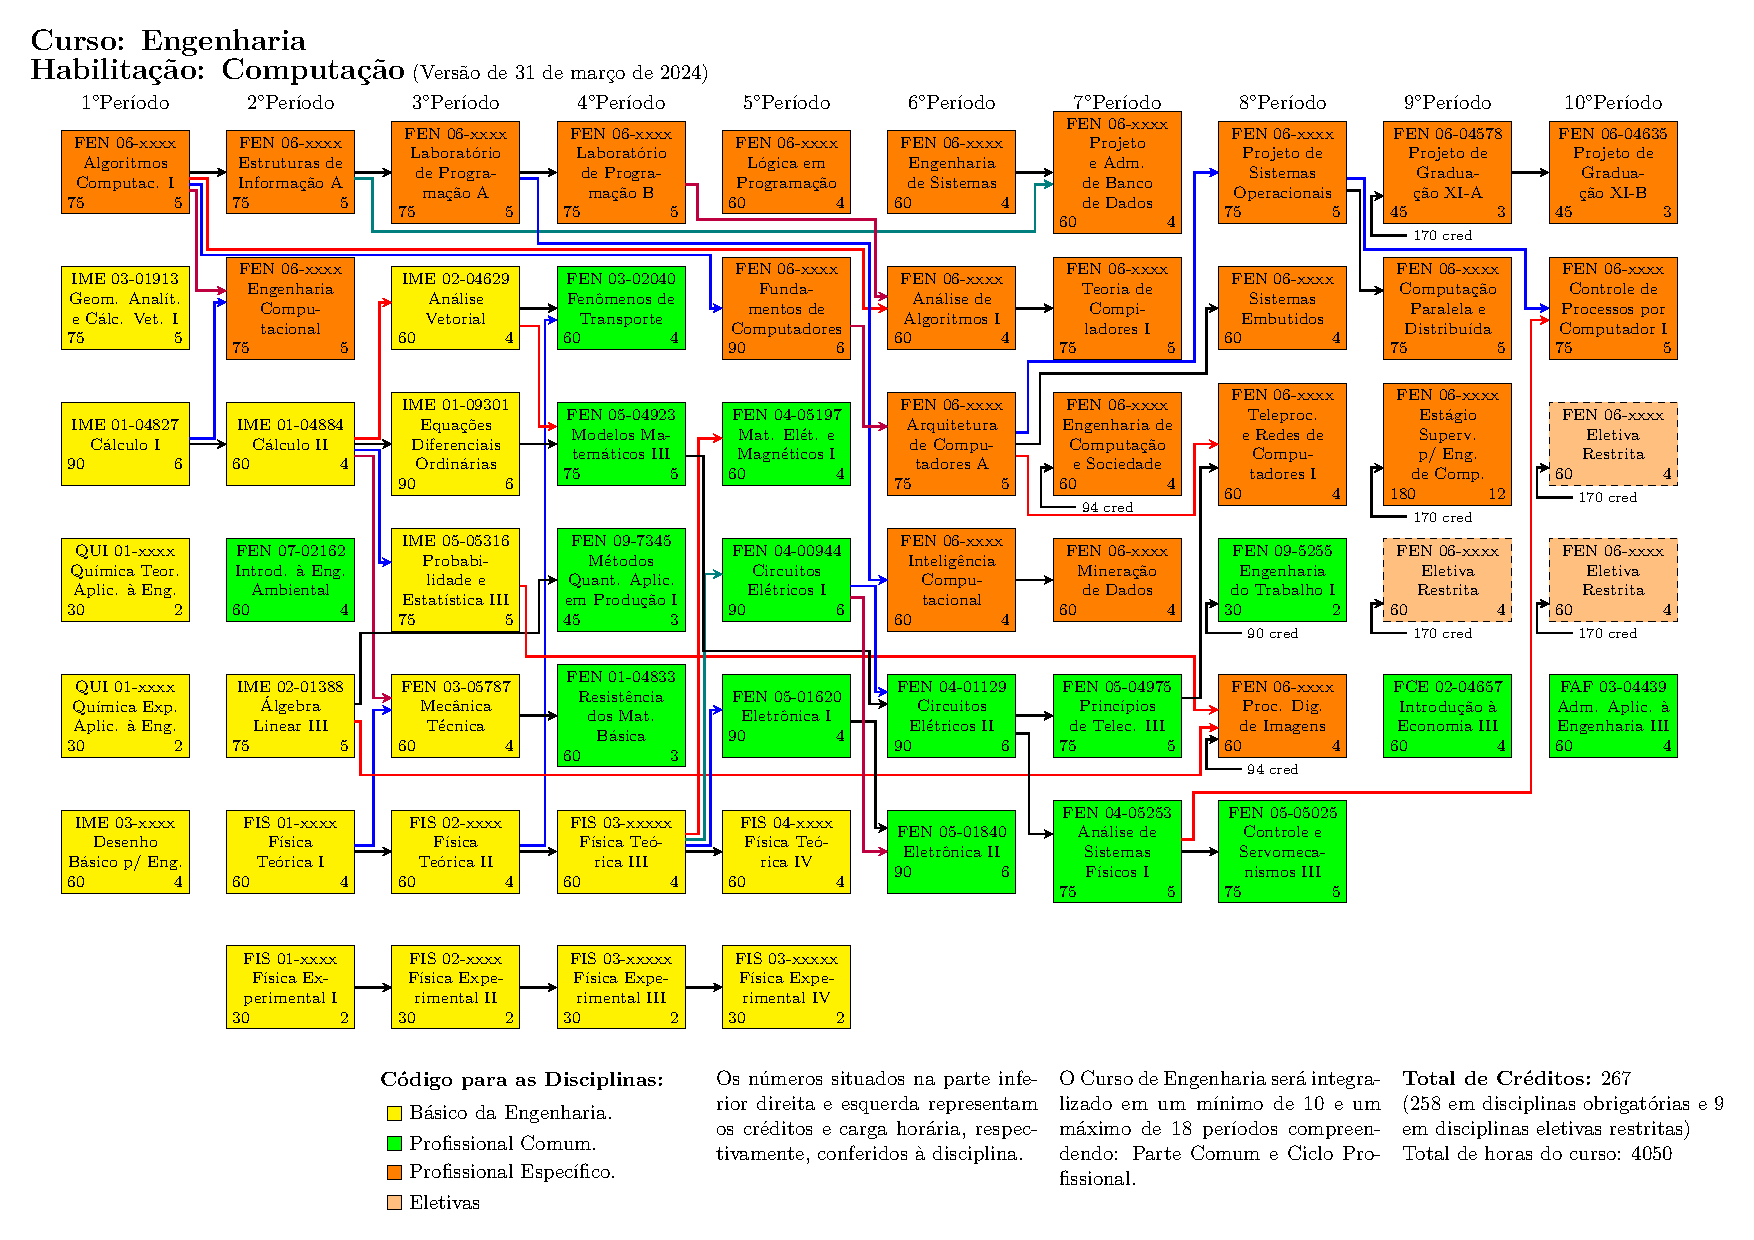
\includepdf[pages=-,angle=90]{fluxogramaEngenhariaComputacao.pdf}
\end{landscape}
\chapter{Ementas do Curso de Engenharia de Computação}
\label{ementas}
\includepdf[pages=-,addtotoc={1,section,1,{\Adm},},pagecommand={\thispagestyle{fancy}}]{ementasExternas/administracao_financeira_de_projeto_assinado.pdf}
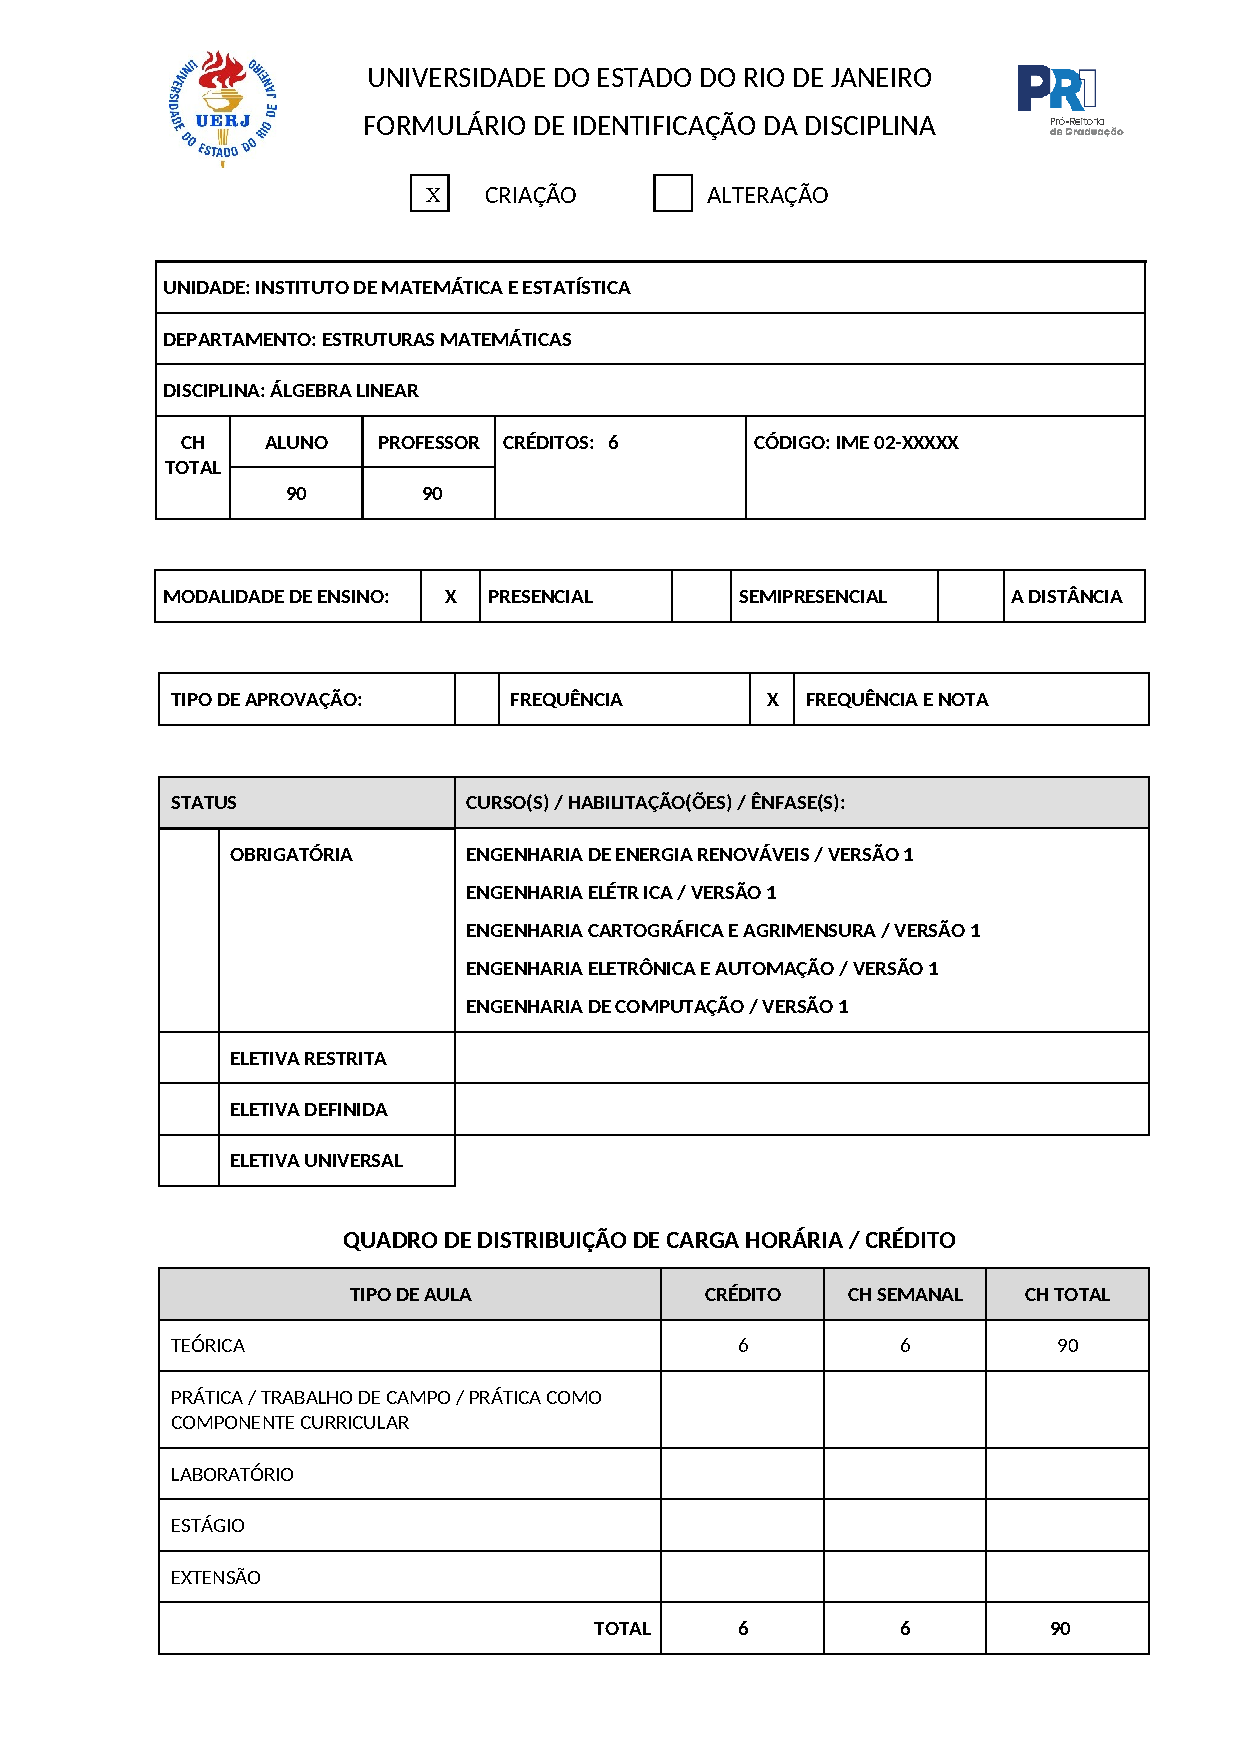
\includepdf[pages=-,addtotoc={1,section,1,{\AlgLin},},pagecommand={\thispagestyle{fancy}}]{ementasExternas/algebra_linear_90hs.pdf}
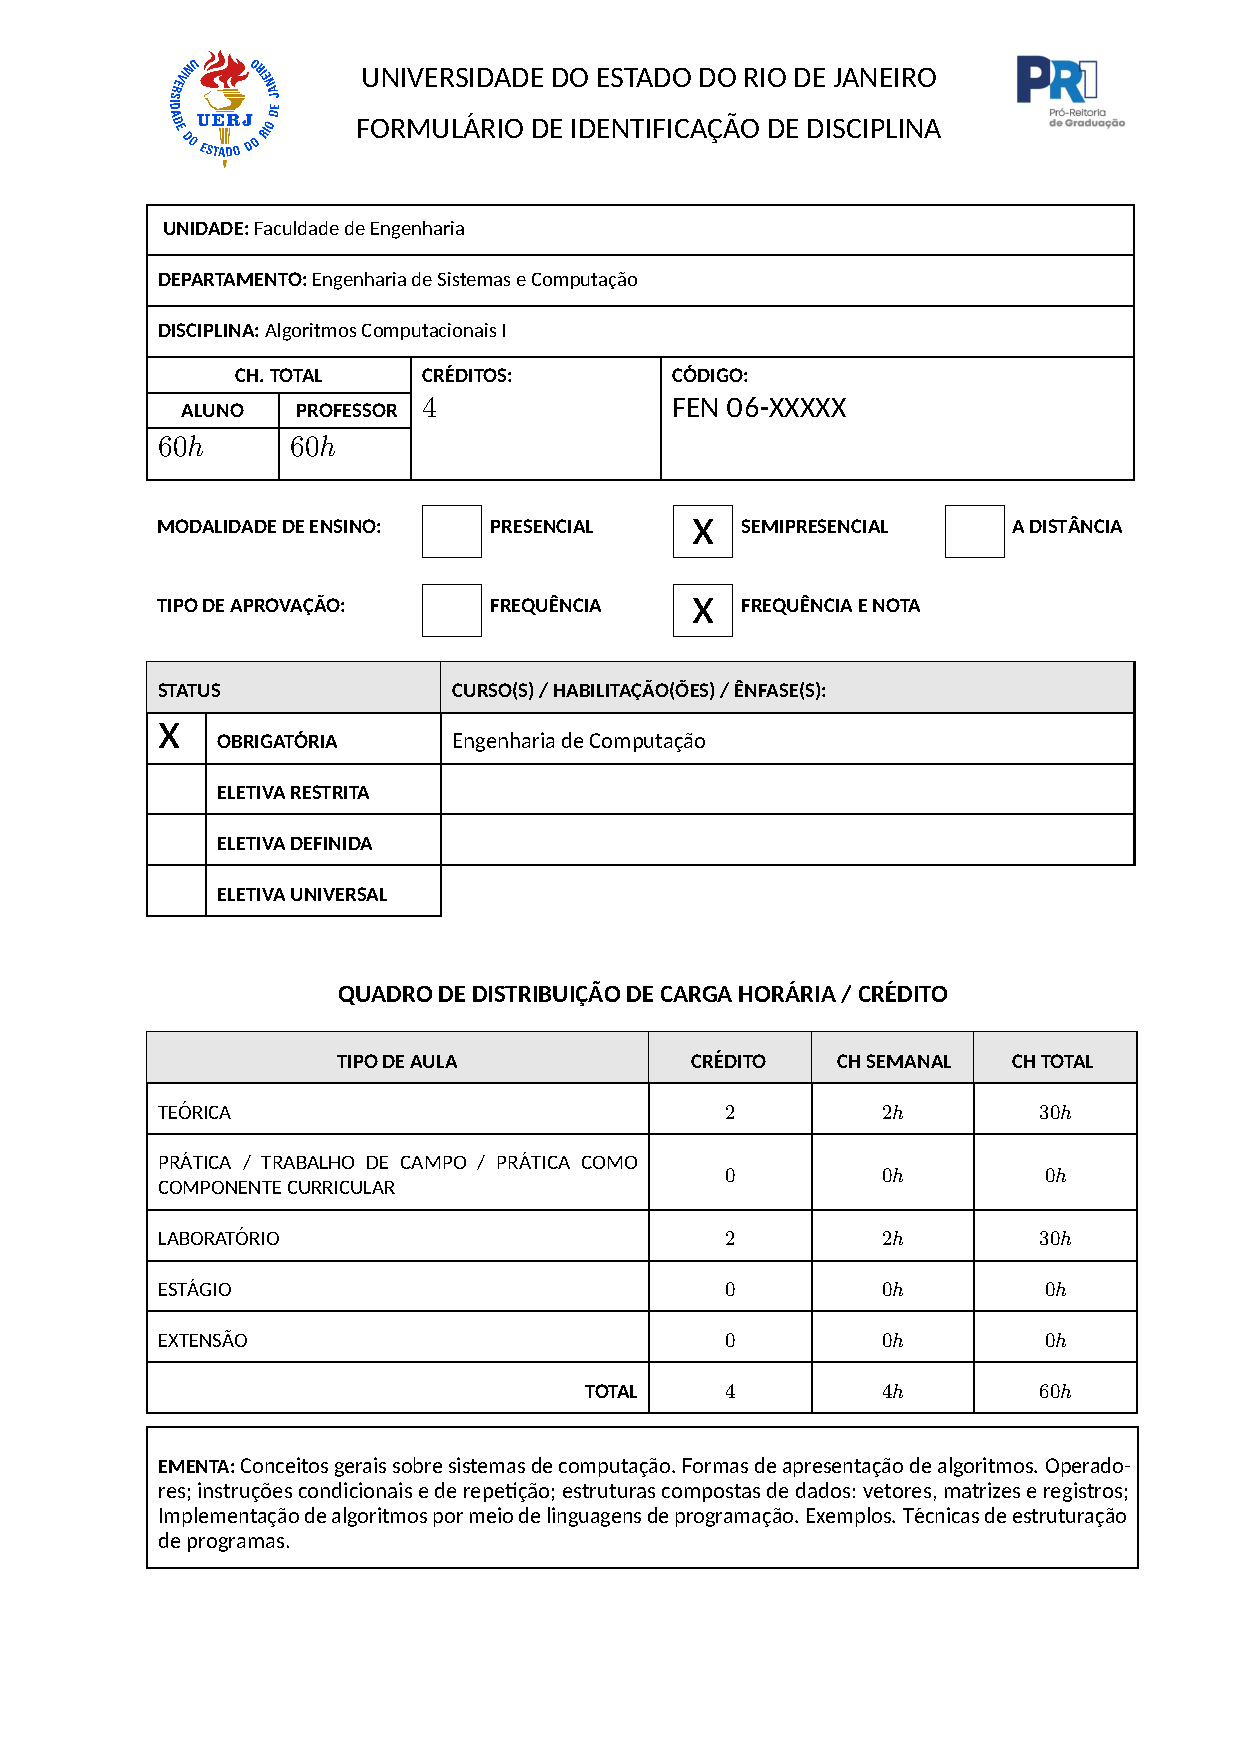
\includepdf[pages=-,addtotoc={1,section,1,{\AlgComp},},pagecommand={\thispagestyle{fancy}}]{ementas/AlgoritmosComputacionais.pdf}
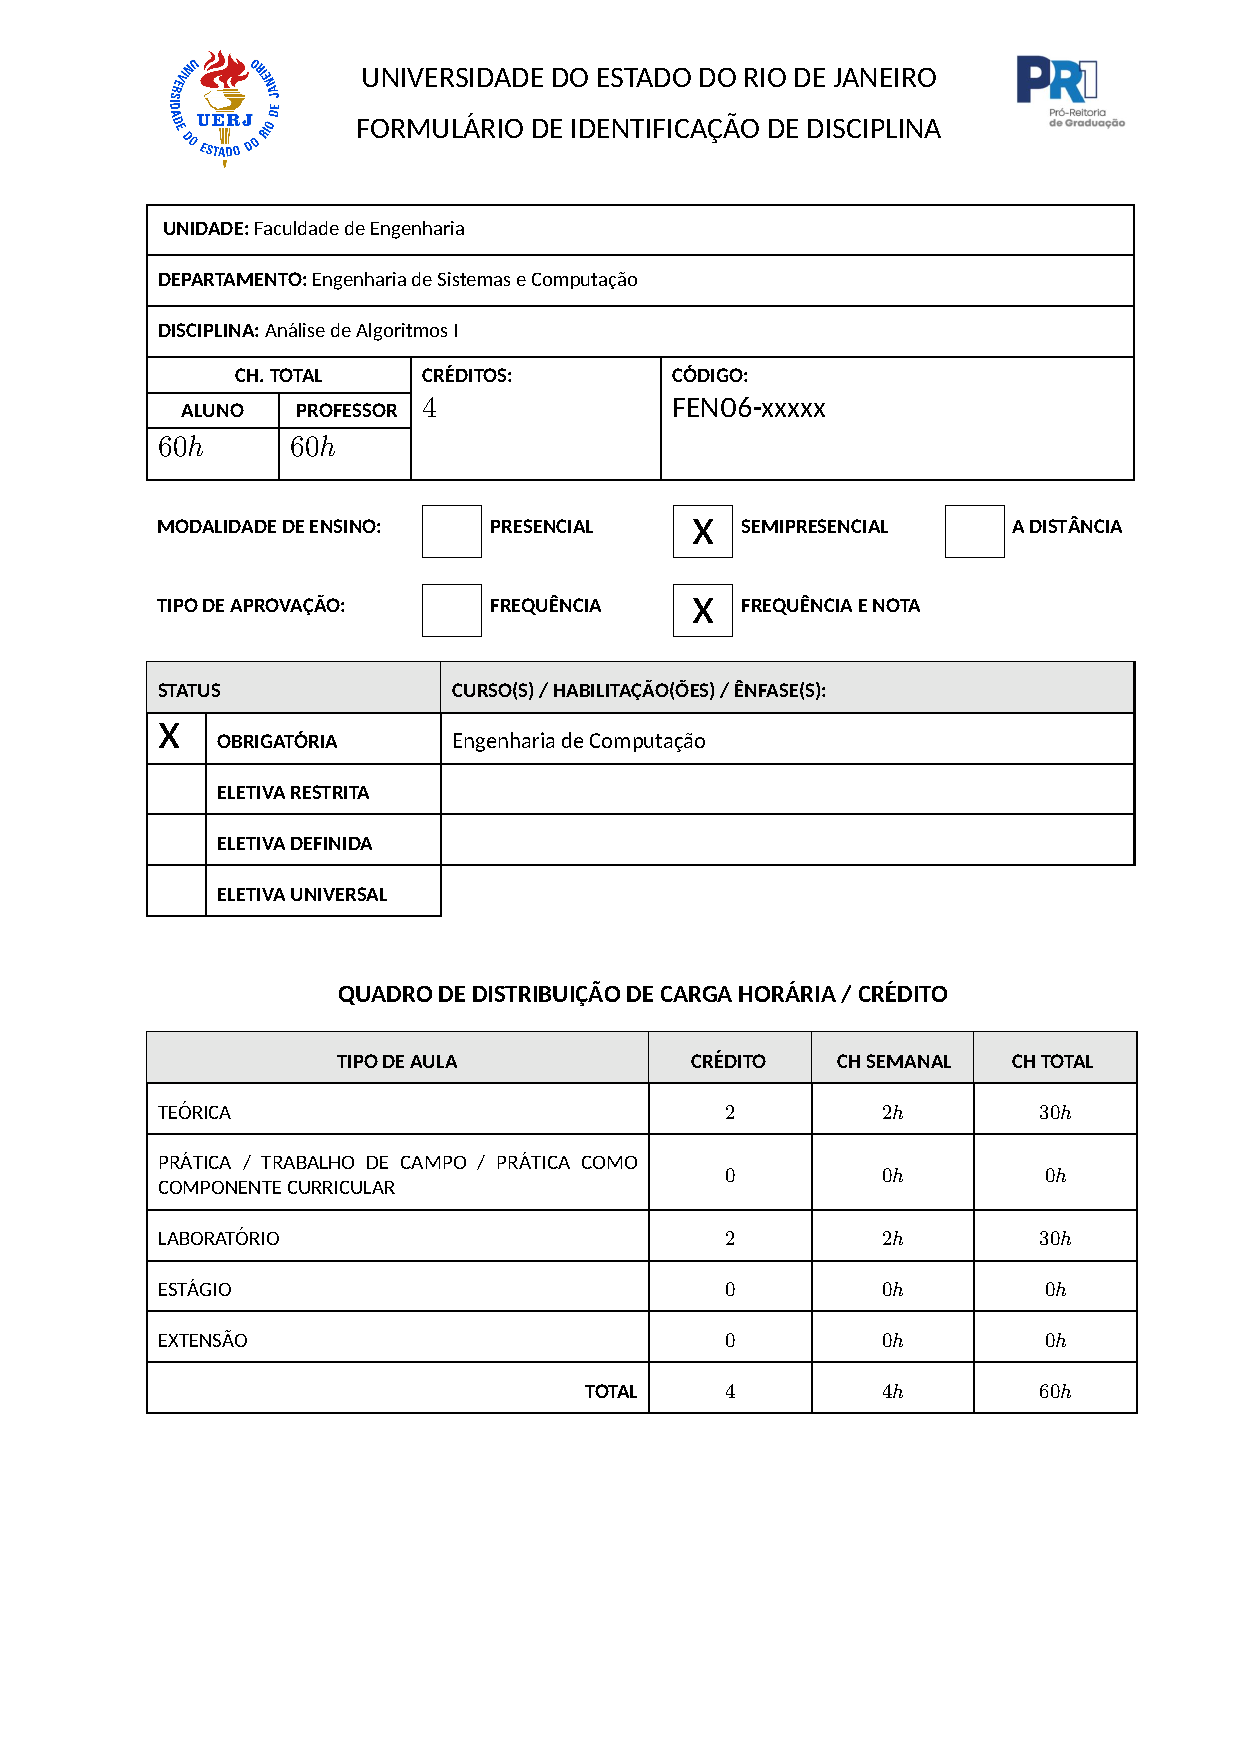
\includepdf[pages=-,addtotoc={1,section,1,{\AnAlg},},pagecommand={\thispagestyle{fancy}}]{ementas/AnaliseDeAlgoritmos.pdf}
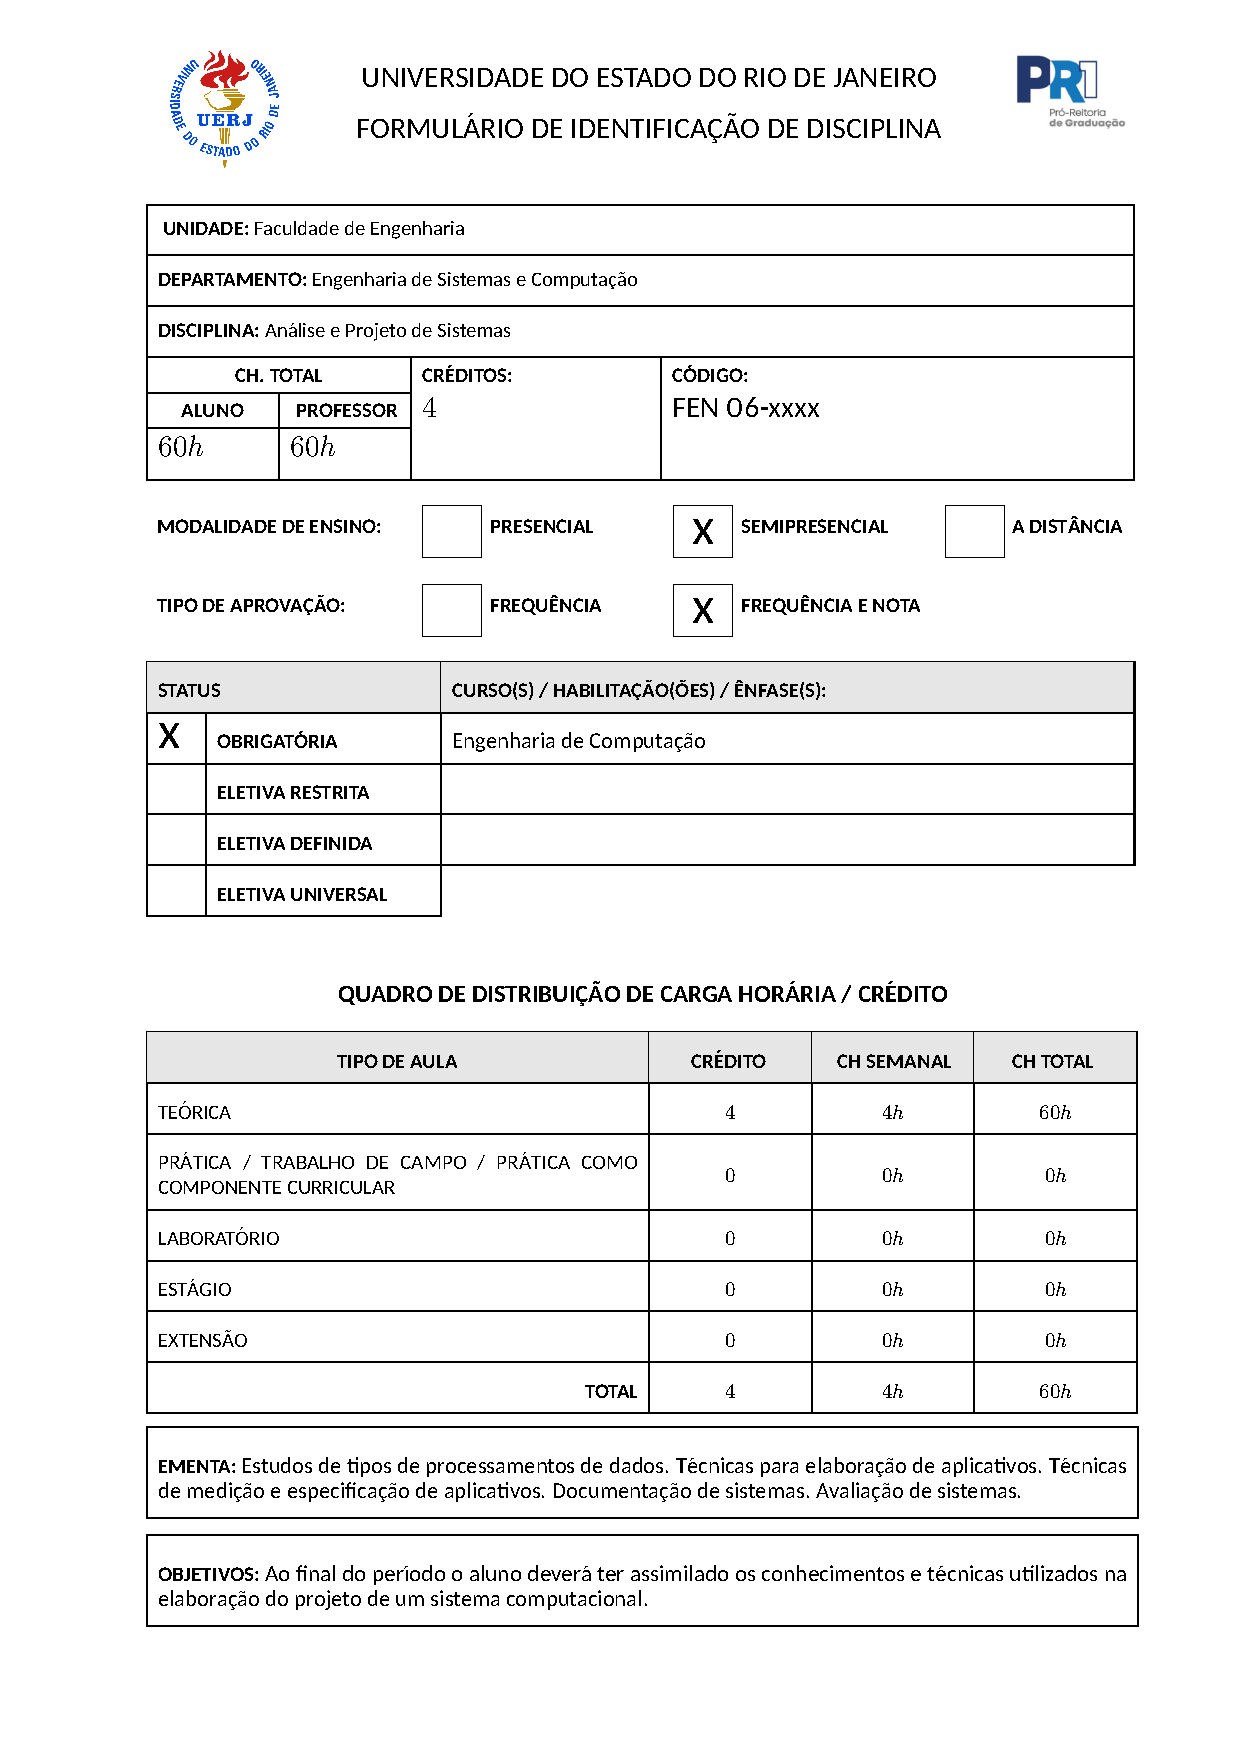
\includepdf[pages=-,addtotoc={1,section,1,{\AnaProjSist},},pagecommand={\thispagestyle{fancy}}]{ementas/analise_e_projeto_de_sistemas.pdf}
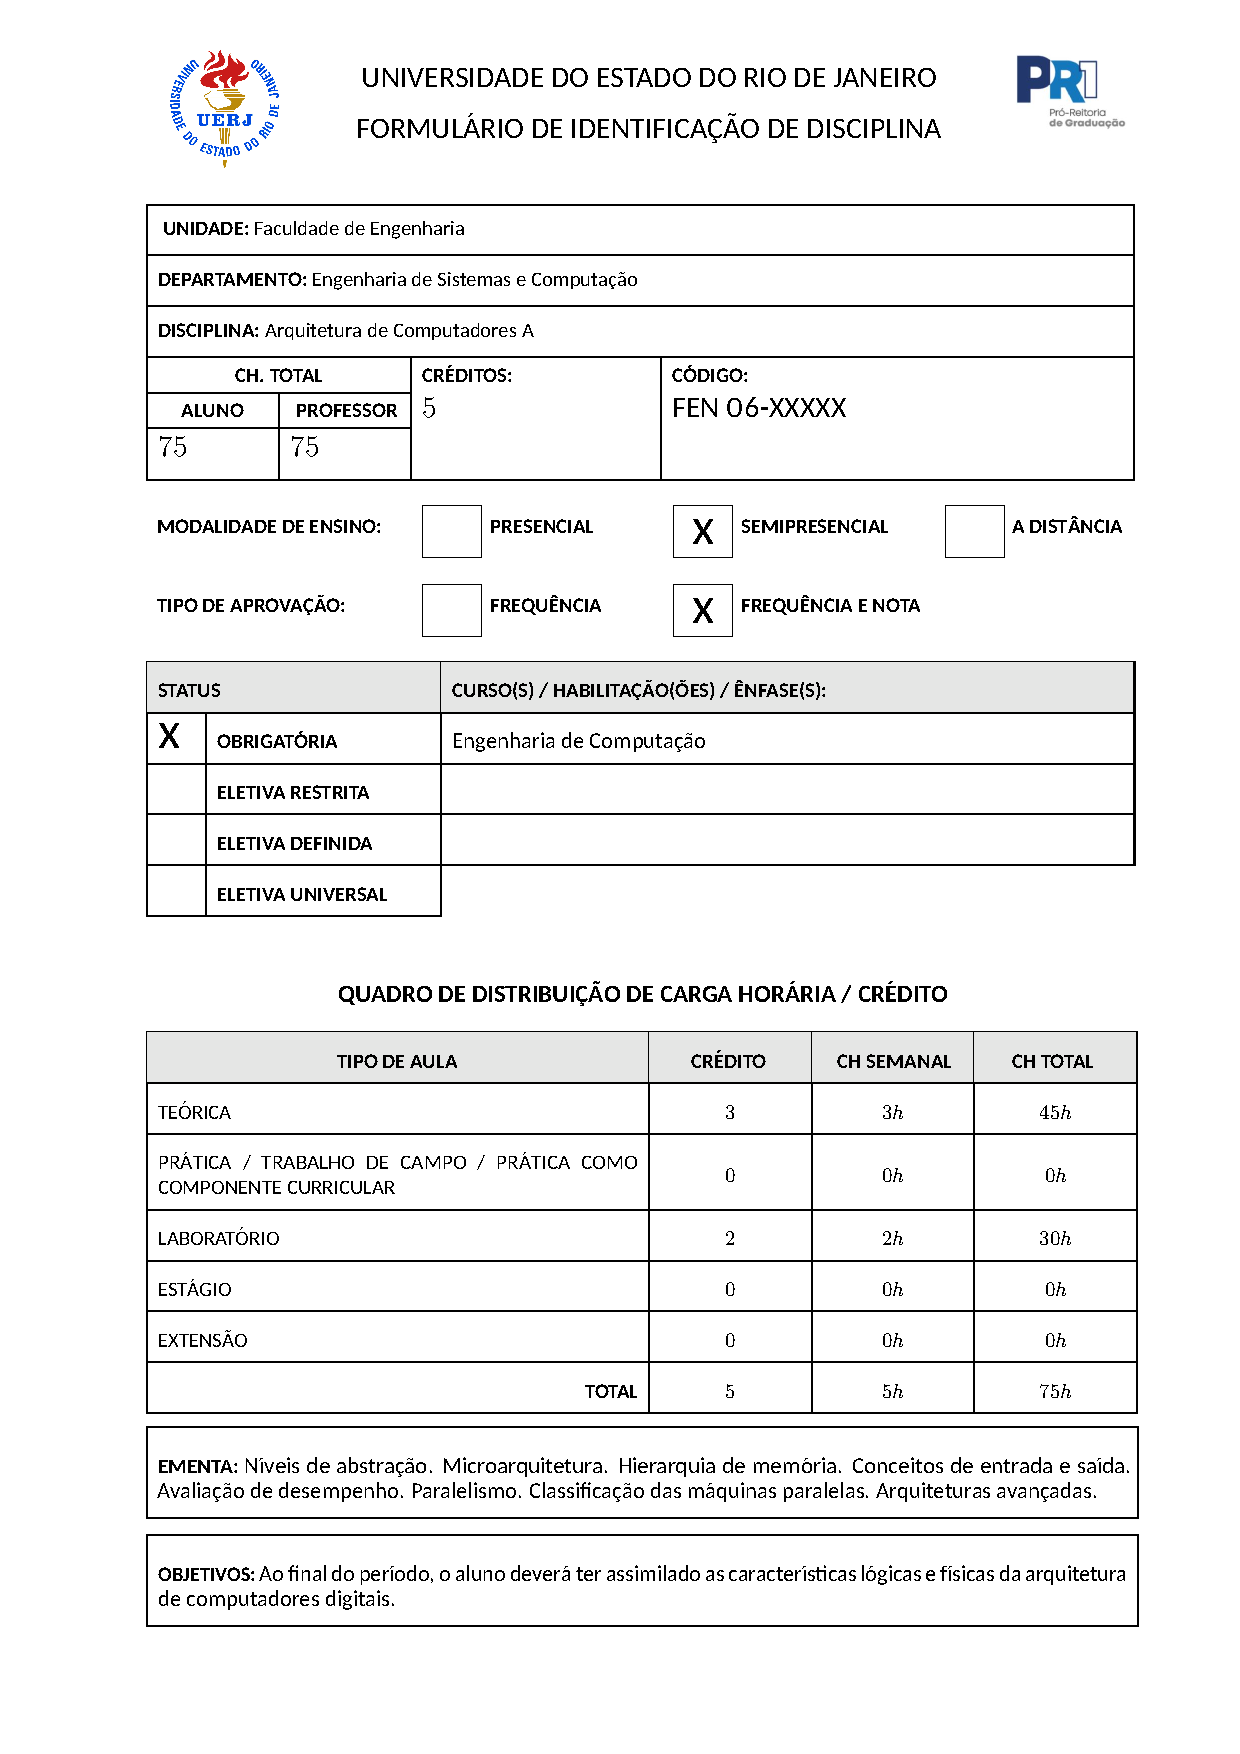
\includepdf[pages=-,addtotoc={1,section,1,{\ArqComp},},pagecommand={\thispagestyle{fancy}}]{ementas/ArquiteturaDeComputadores.pdf}
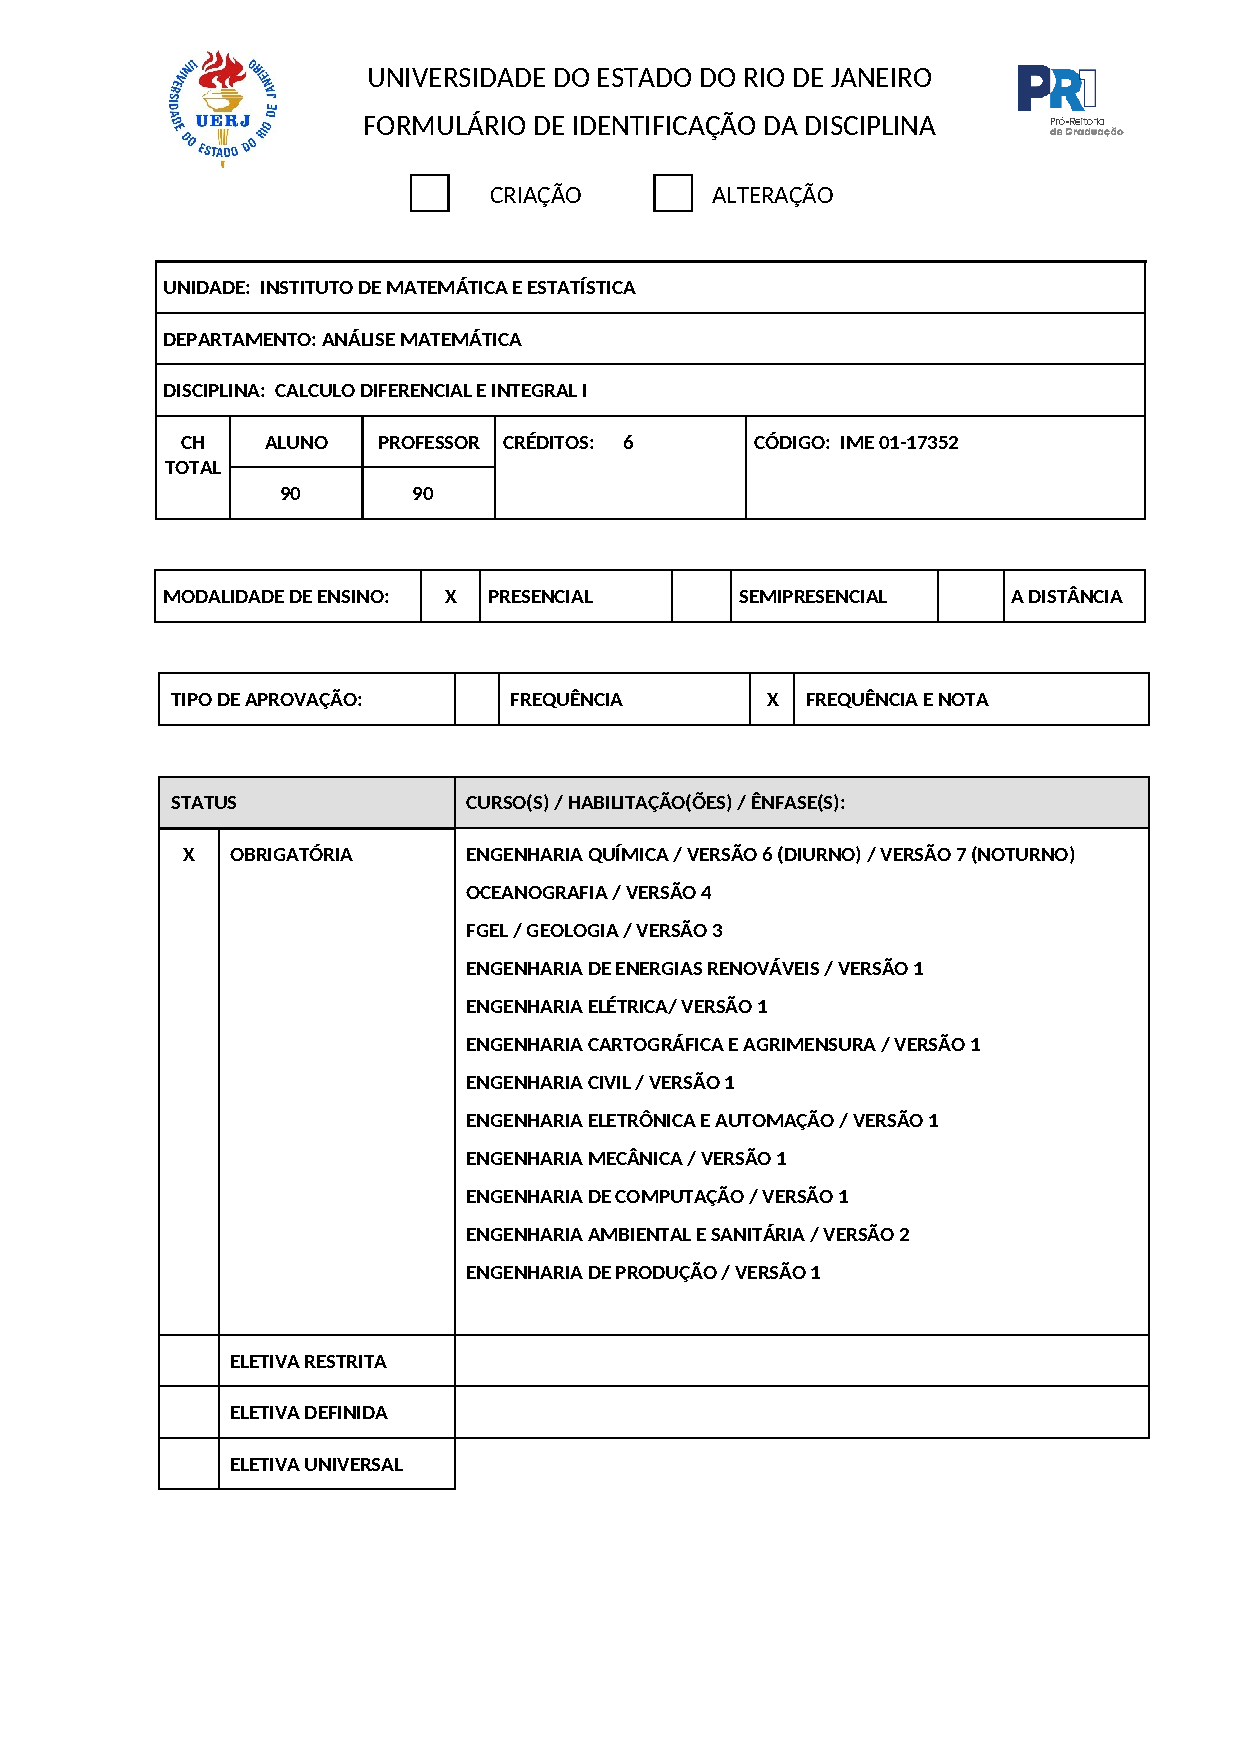
\includepdf[pages=-,addtotoc={1,section,1,{\CalcI},},pagecommand={\thispagestyle{fancy}}]{ementasExternas/calculo_diferencial_e_integral_i.pdf}
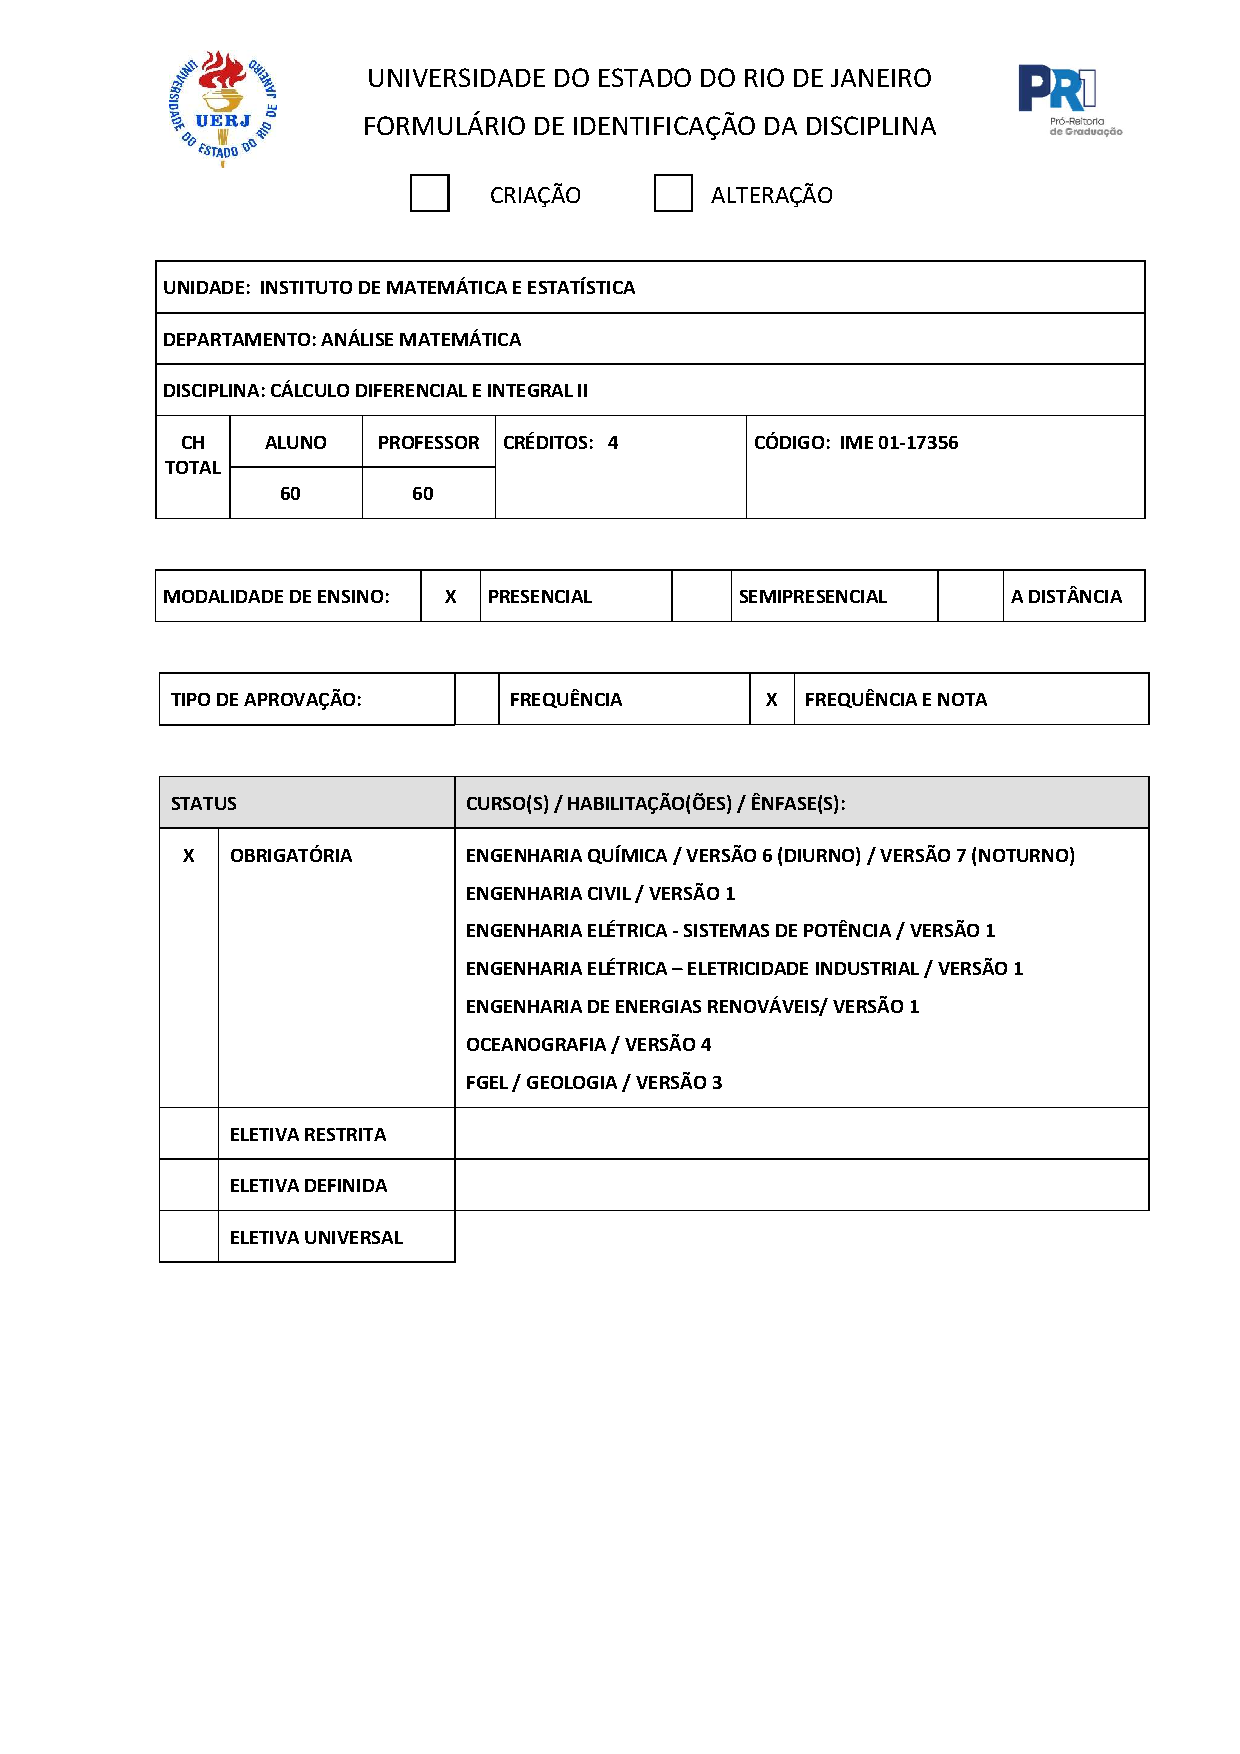
\includepdf[pages=-,addtotoc={1,section,1,{\CalcII},},pagecommand={\thispagestyle{fancy}}]{ementasExternas/calculo_diferencial_e_integral_ii.pdf}
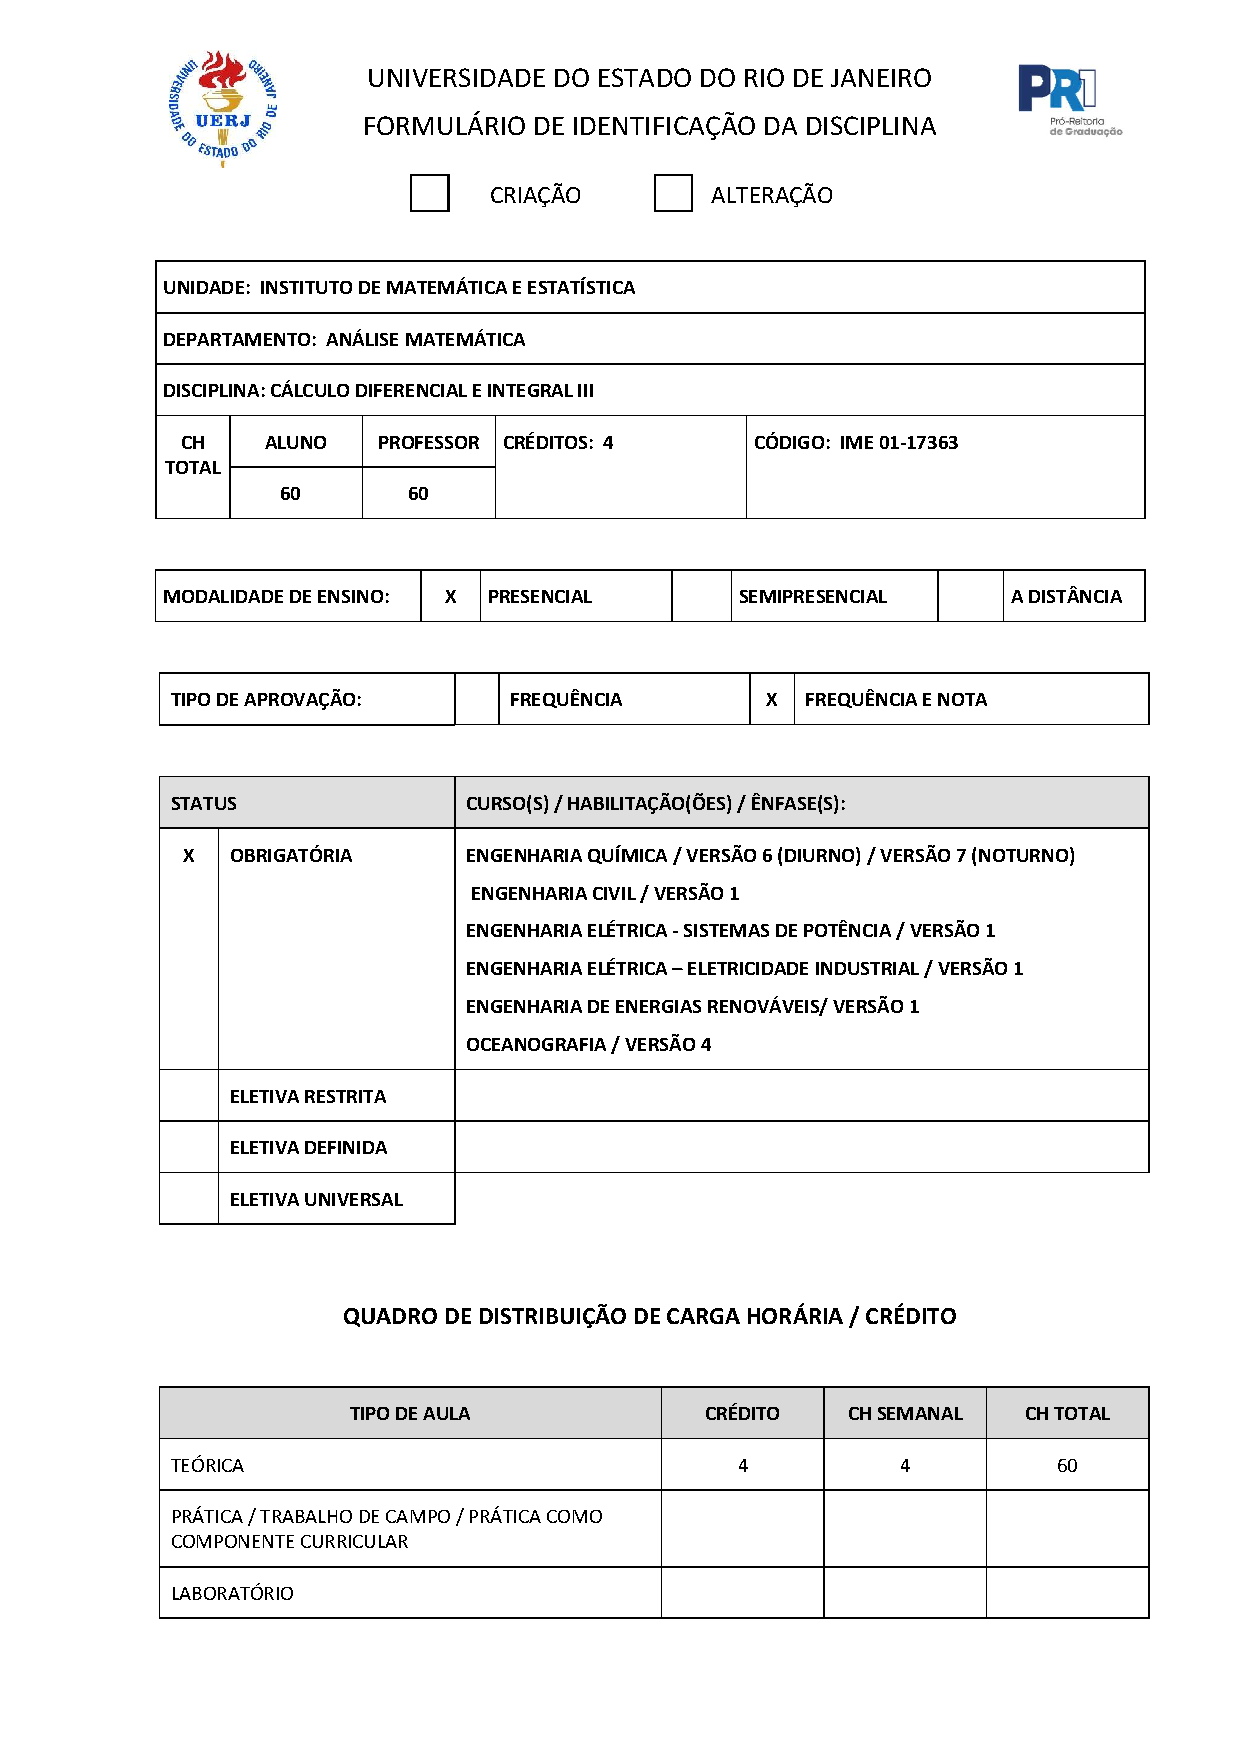
\includepdf[pages=-,addtotoc={1,section,1,{\CalcIII},},pagecommand={\thispagestyle{fancy}}]{ementasExternas/calculo_diferencial_e_integral_iii.pdf}
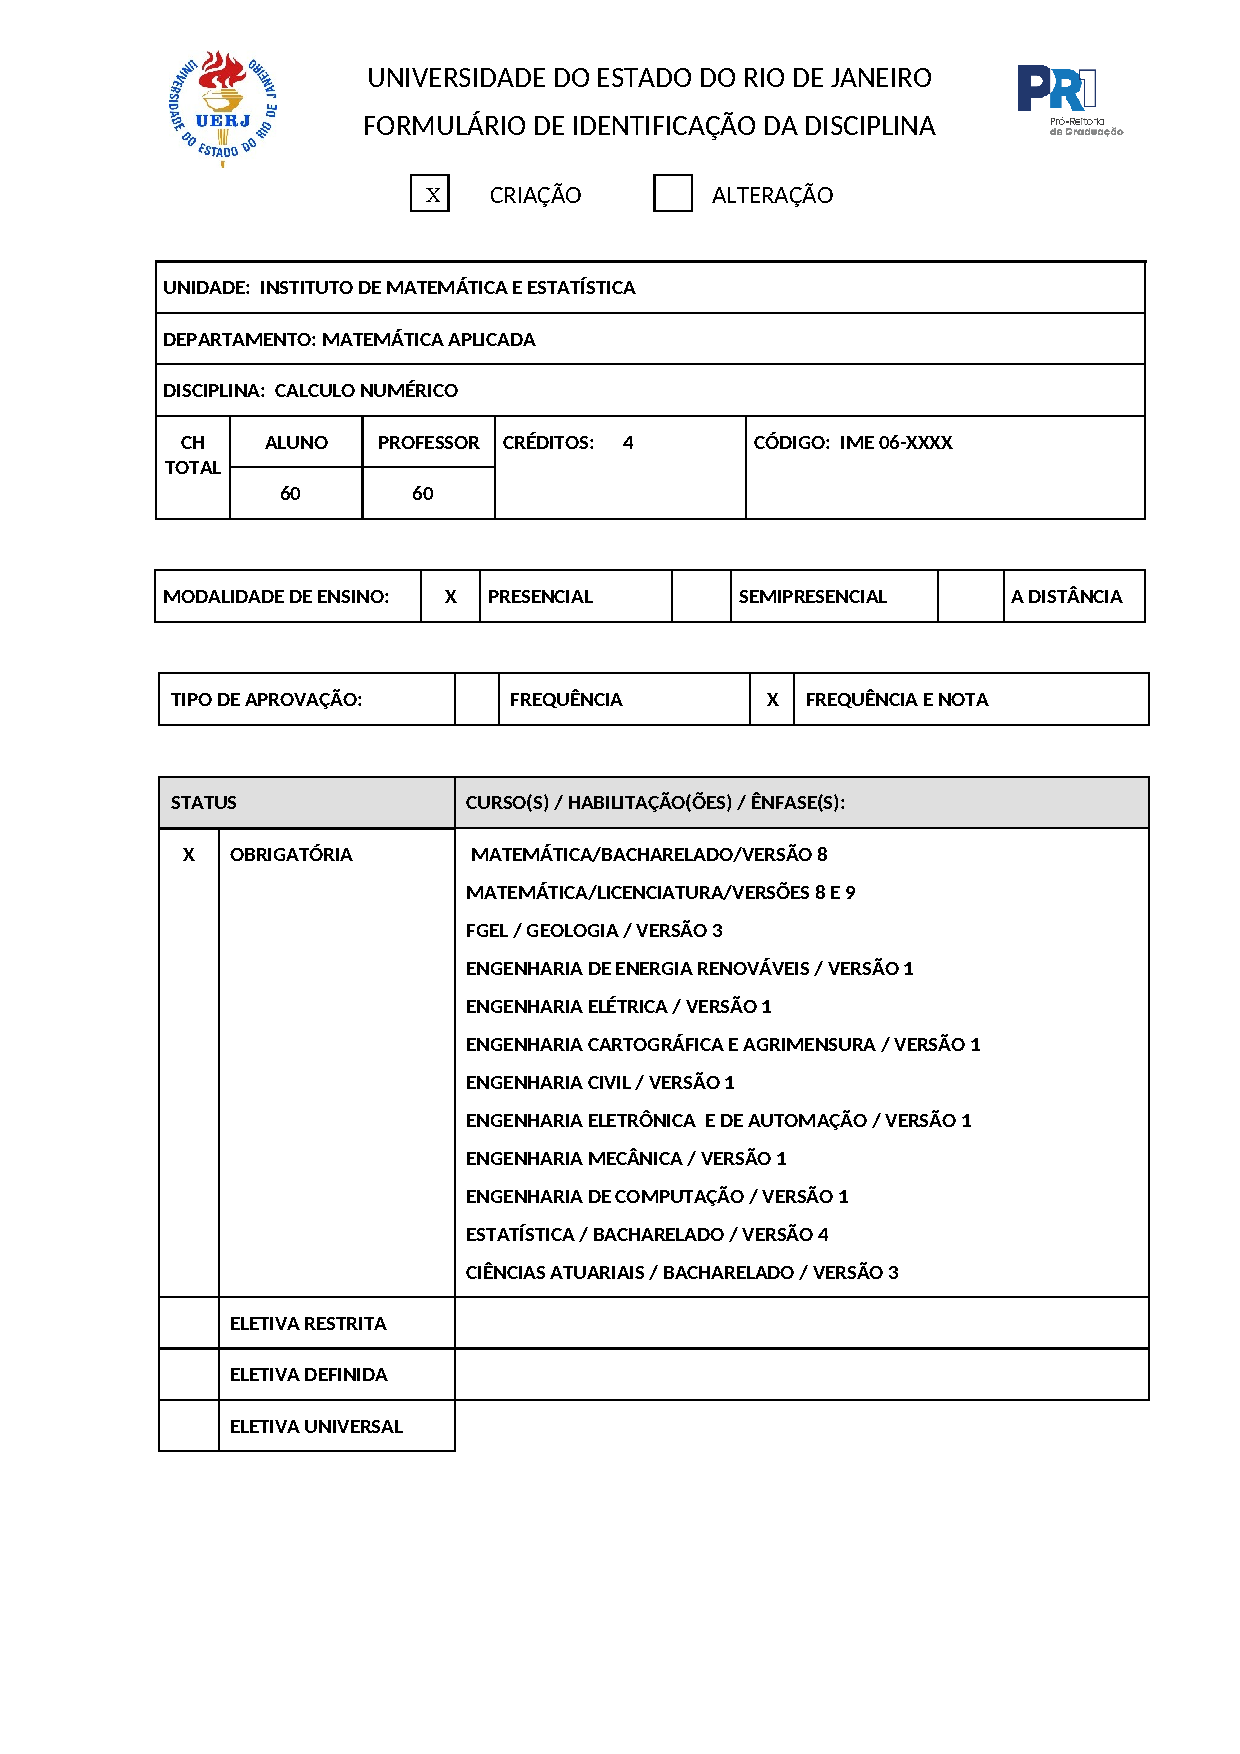
\includepdf[pages=-,addtotoc={1,section,1,{\CalcNum},},pagecommand={\thispagestyle{fancy}}]{ementasExternas/Calculo_Numerico.pdf}
\includepdf[pages=-,addtotoc={1,section,1,{\CircEletI},},pagecommand={\thispagestyle{fancy}}]{ementasExternas/FEN05-Circuitos_Eletronicos_I_assinado.pdf}% Circuitos Eletrônicos I
\includepdf[pages=-,addtotoc={1,section,1,{\CCA},},pagecommand={\thispagestyle{fancy}}]{ementasExternas/FEN04_circuitos_em_corrente_alternada_assinado.pdf}
\includepdf[pages=-,addtotoc={1,section,1,{\CCC},},pagecommand={\thispagestyle{fancy}}]{ementasExternas/FEN04_circuitos_em_corrente_continua_assinado.pdf}
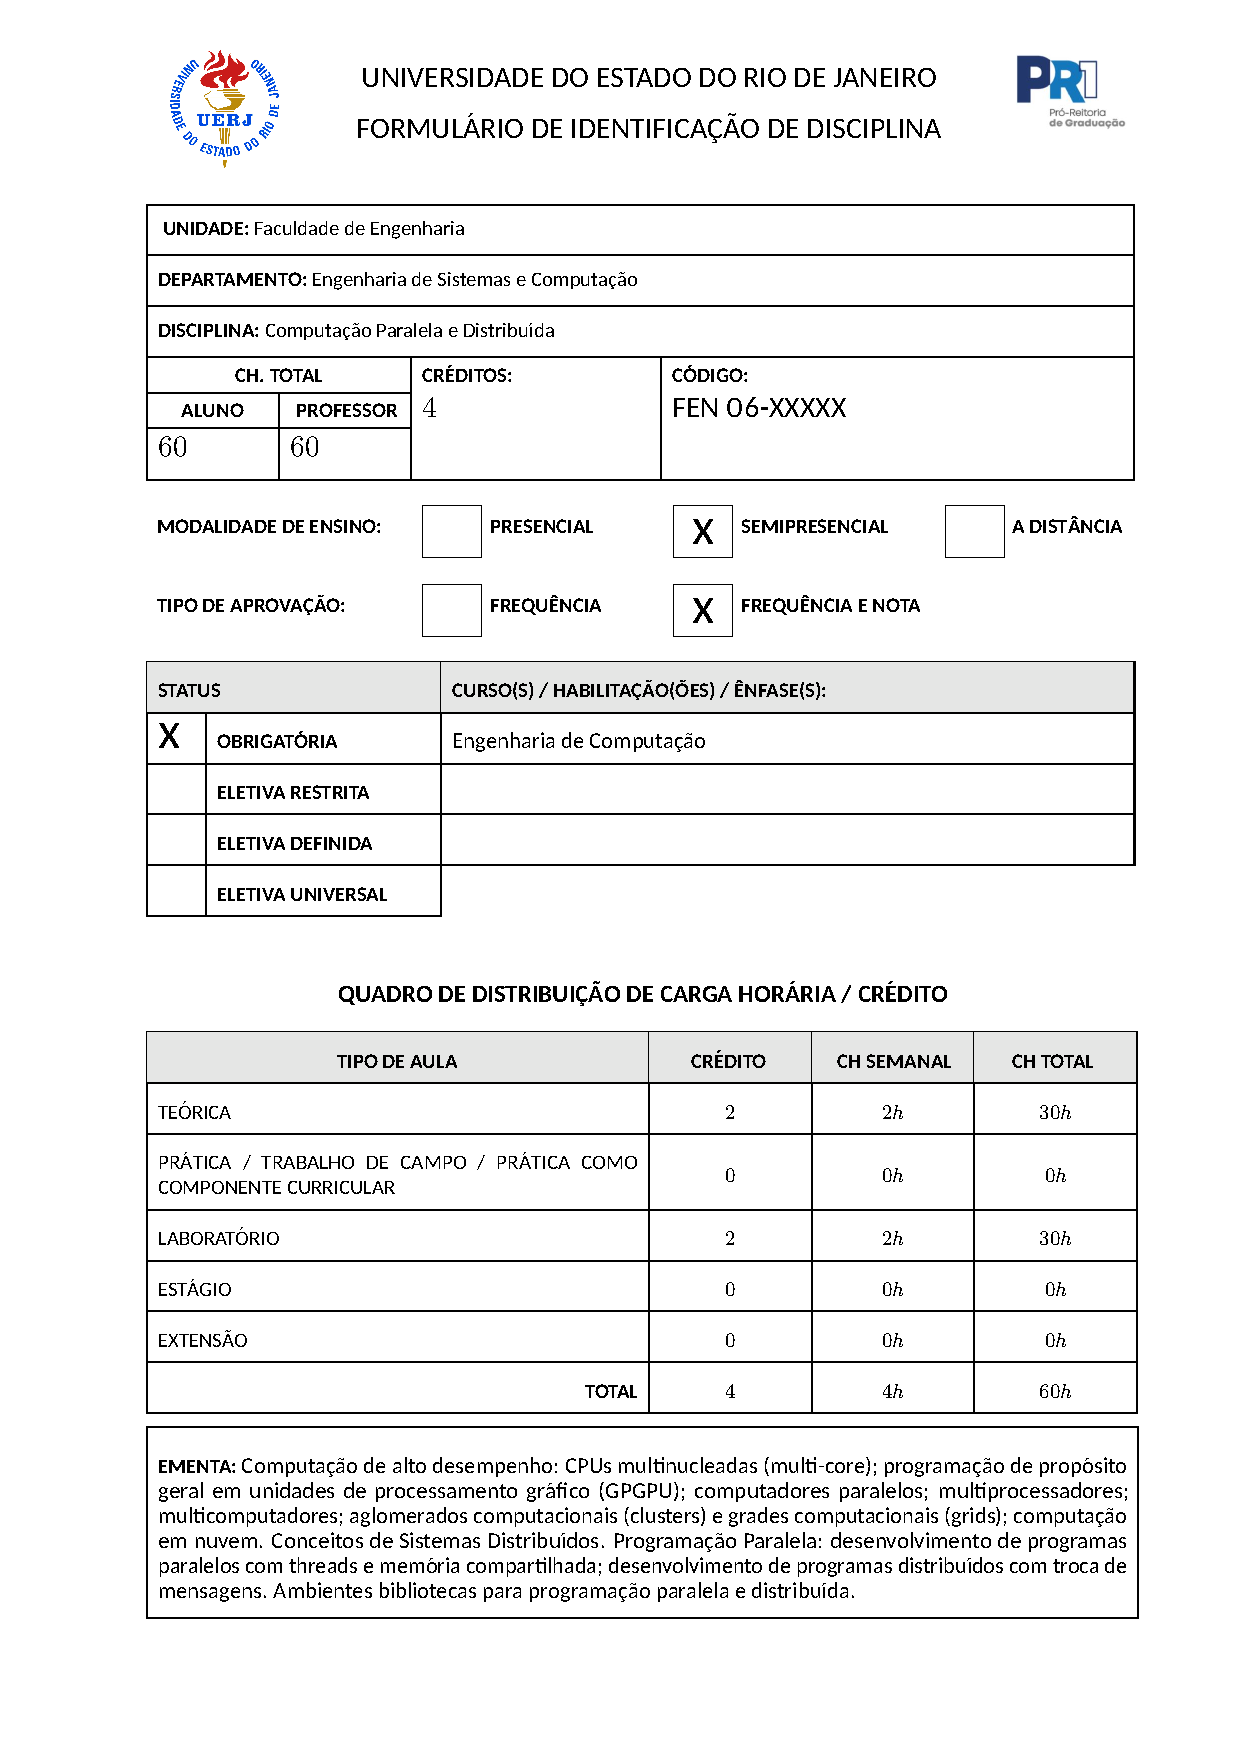
\includepdf[pages=-,addtotoc={1,section,1,{\CompParal},},pagecommand={\thispagestyle{fancy}}]{ementas/ComputacaoParalela.pdf}
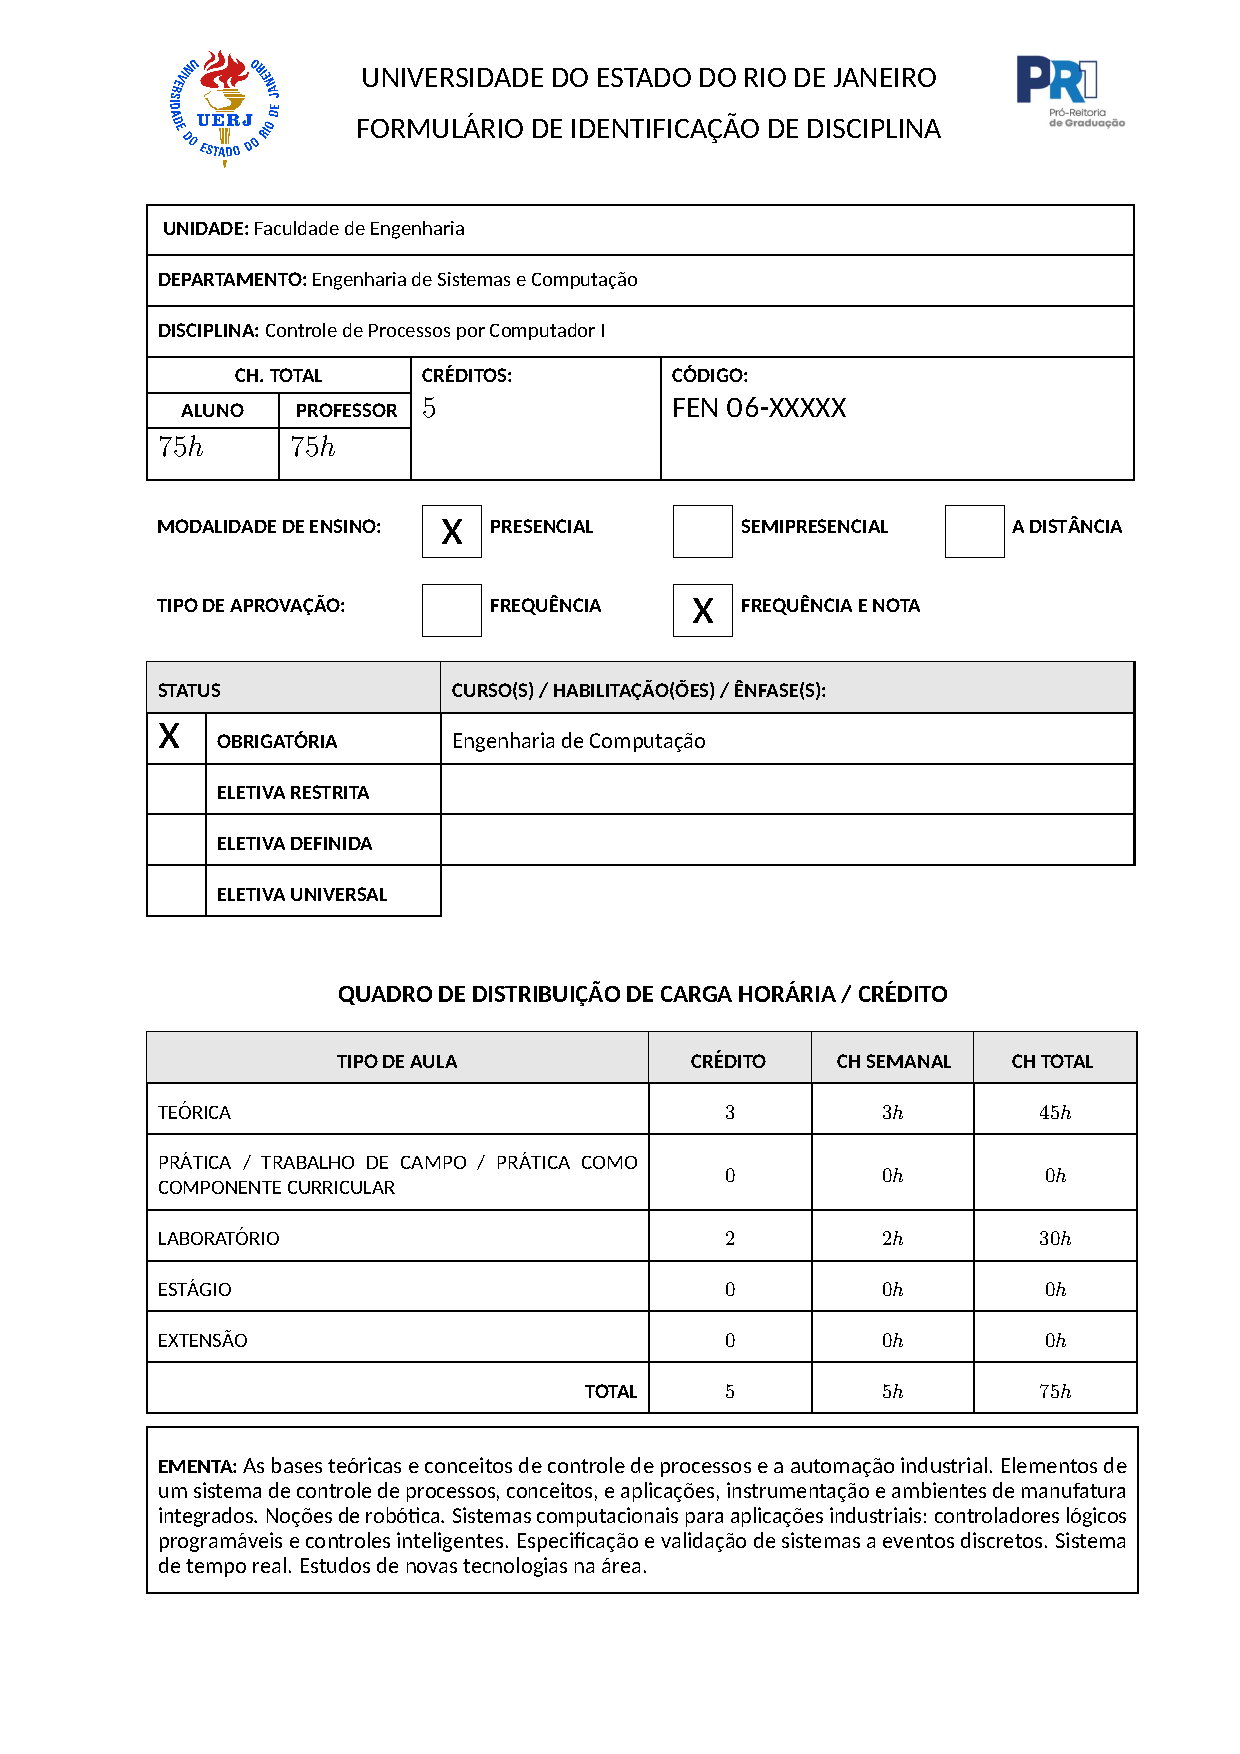
\includepdf[pages=-,addtotoc={1,section,1,{\Control},},pagecommand={\thispagestyle{fancy}}]{ementas/ControleDeProcessosPorComputador.pdf}
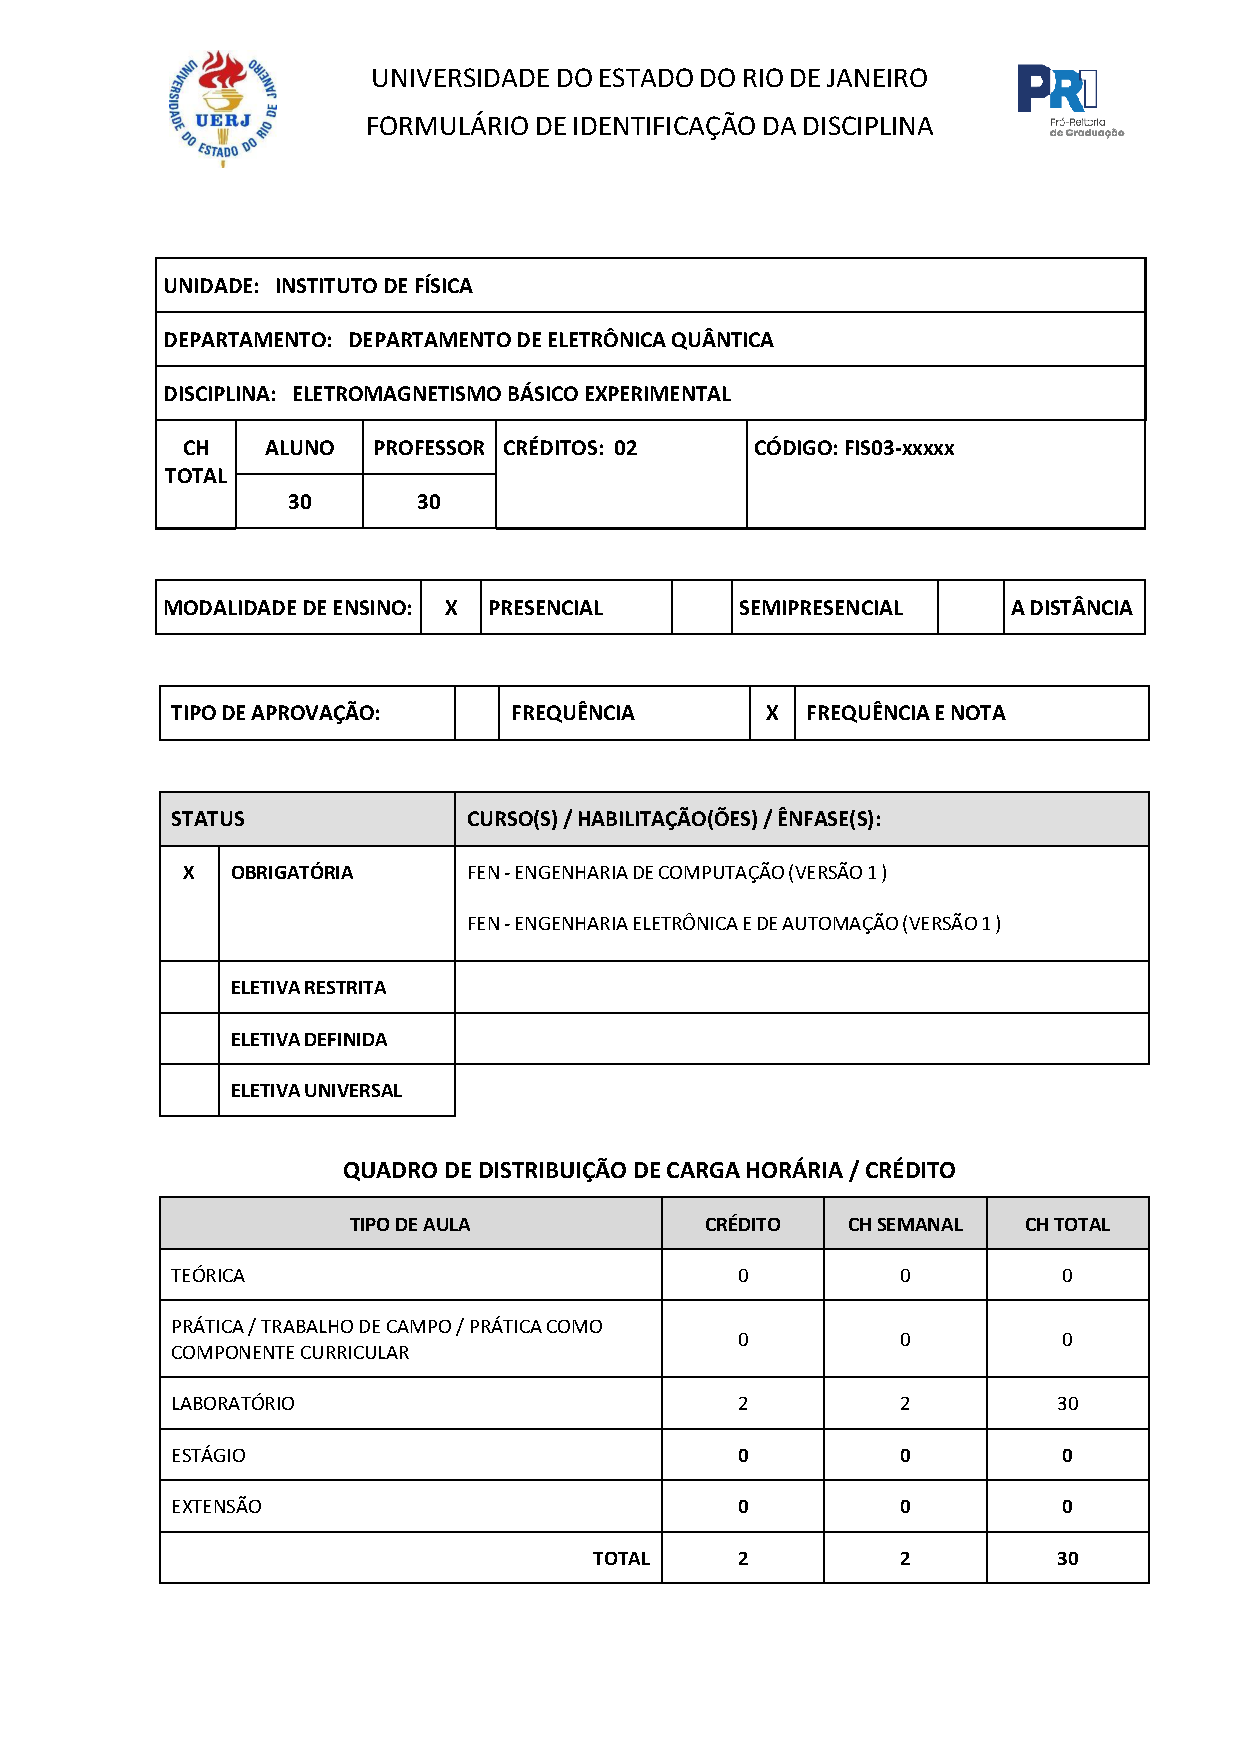
\includepdf[pages=-,addtotoc={1,section,1,{\FisIII},},pagecommand={\thispagestyle{fancy}}]{ementasExternas/FIS03-eletromagnetismo_basico_experimental.pdf}
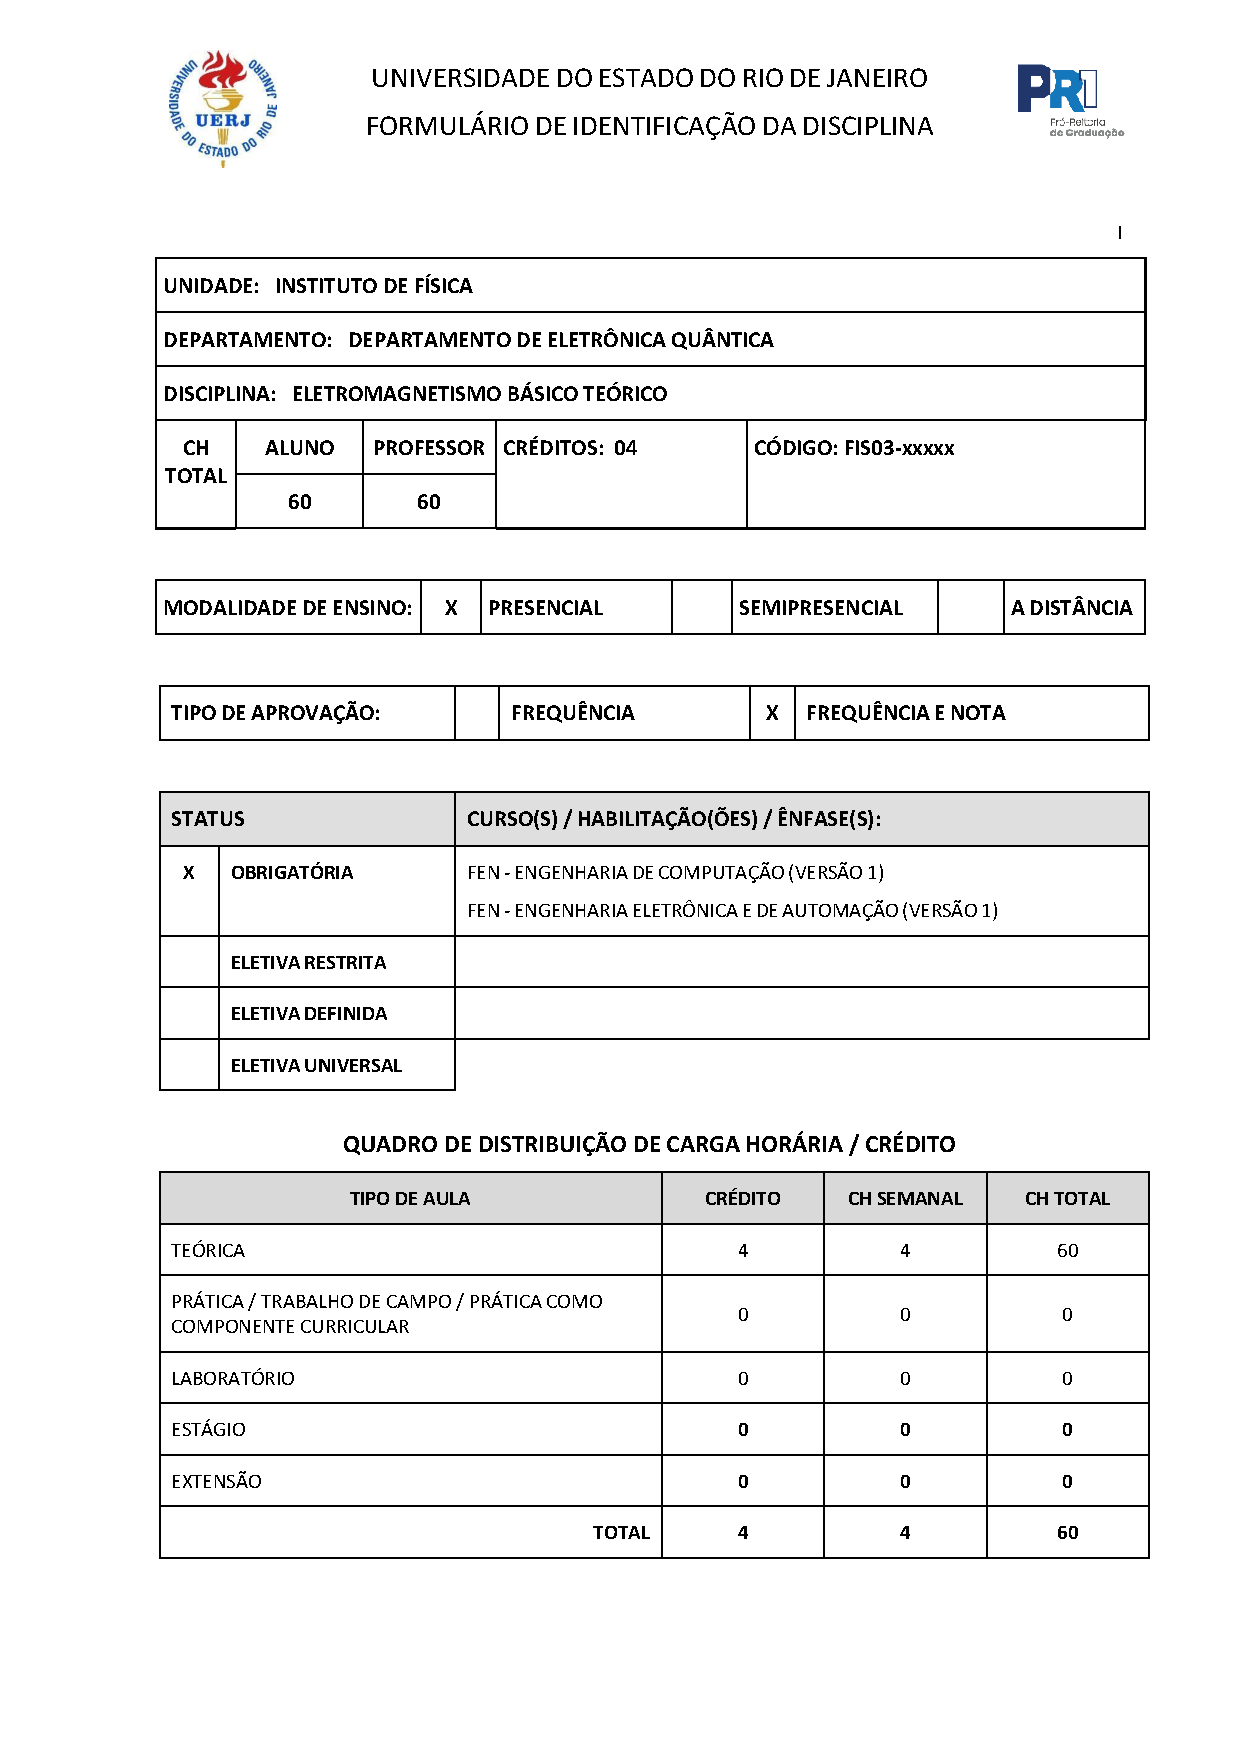
\includepdf[pages=-,addtotoc={1,section,1,{\FisEIII},},pagecommand={\thispagestyle{fancy}}]{ementasExternas/FIS03-eletromagnetismo_basico_teorico.pdf}
\includepdf[pages=-,addtotoc={1,section,1,{\Empre},},pagecommand={\thispagestyle{fancy}}]{ementasExternas/empreendedorismo_na_engenharia_assinado.pdf}
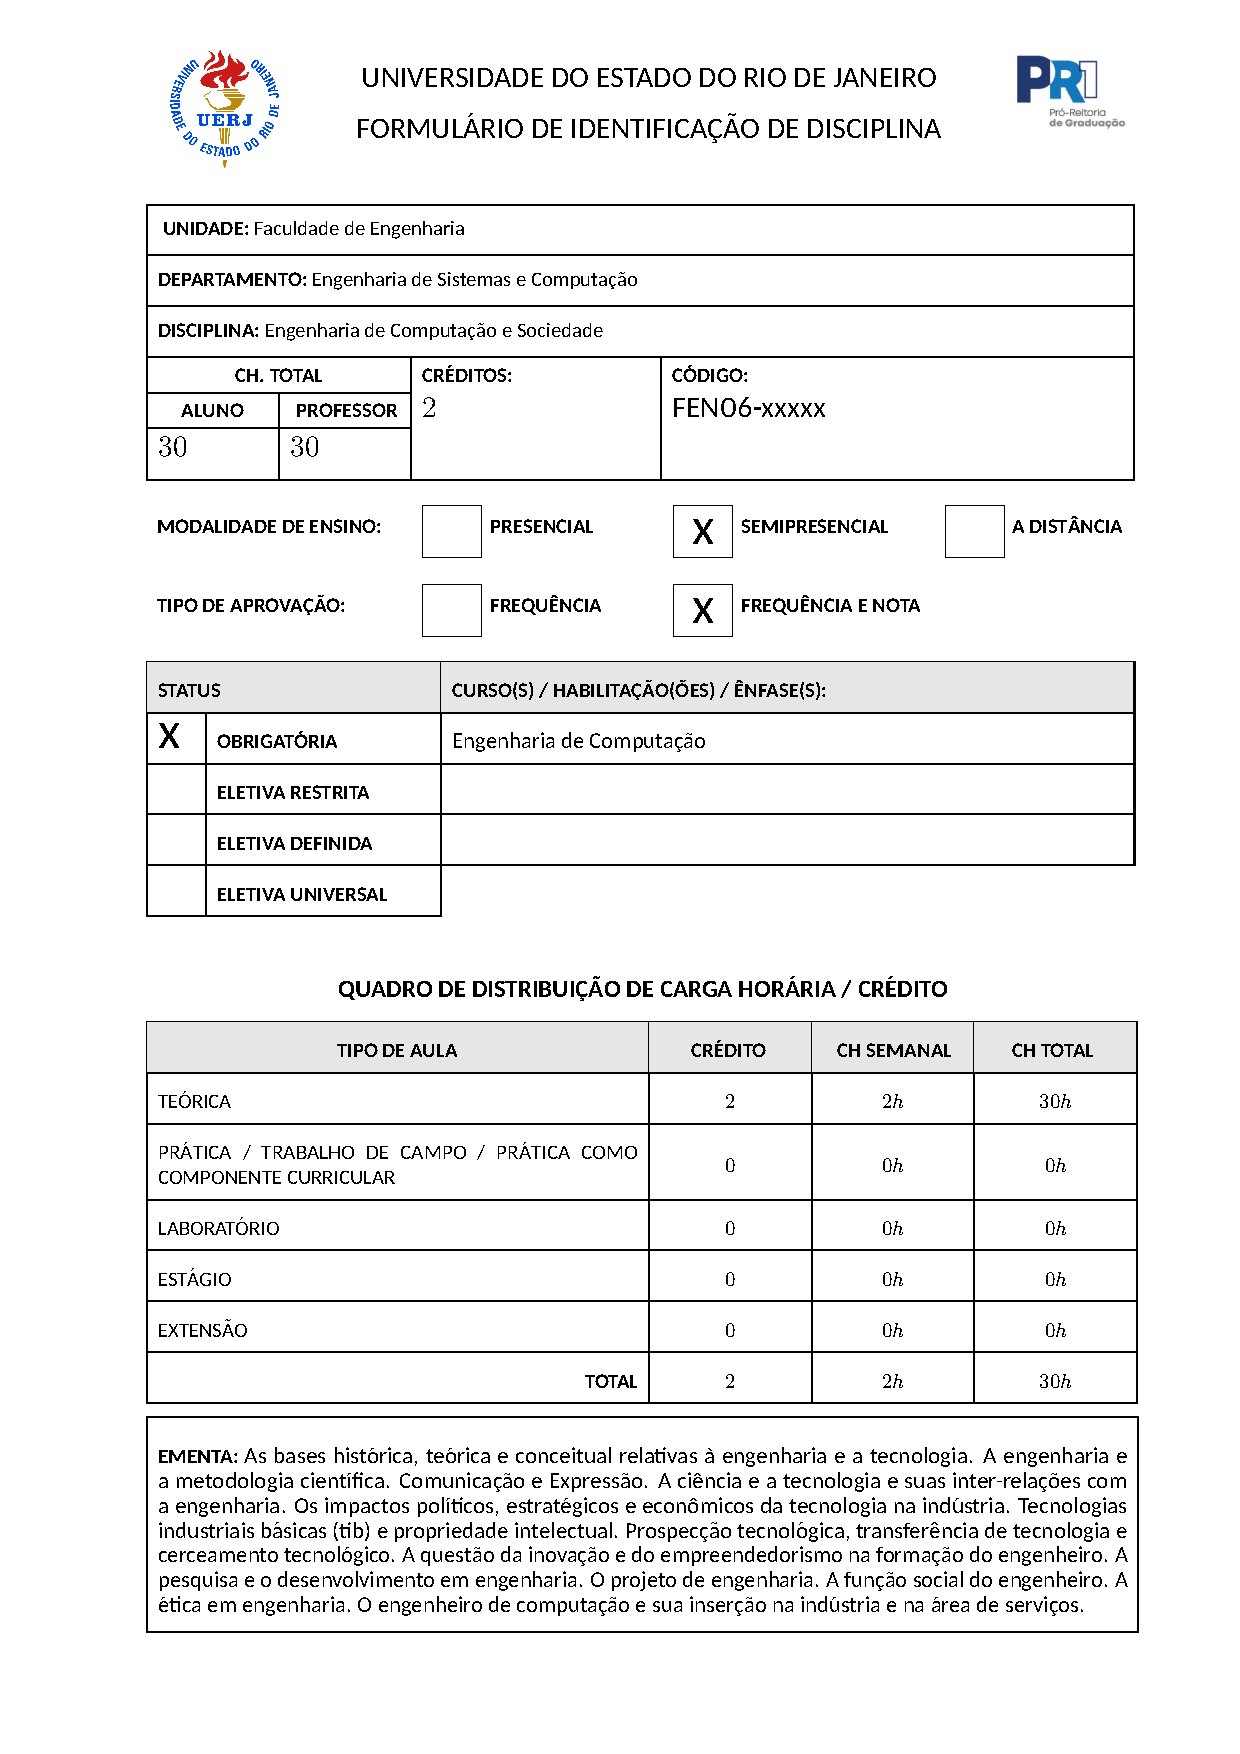
\includepdf[pages=-,addtotoc={1,section,1,{\EngCompSoc},},pagecommand={\thispagestyle{fancy}}]{ementas/EngenhariaDeComputacaoESociedade.pdf}
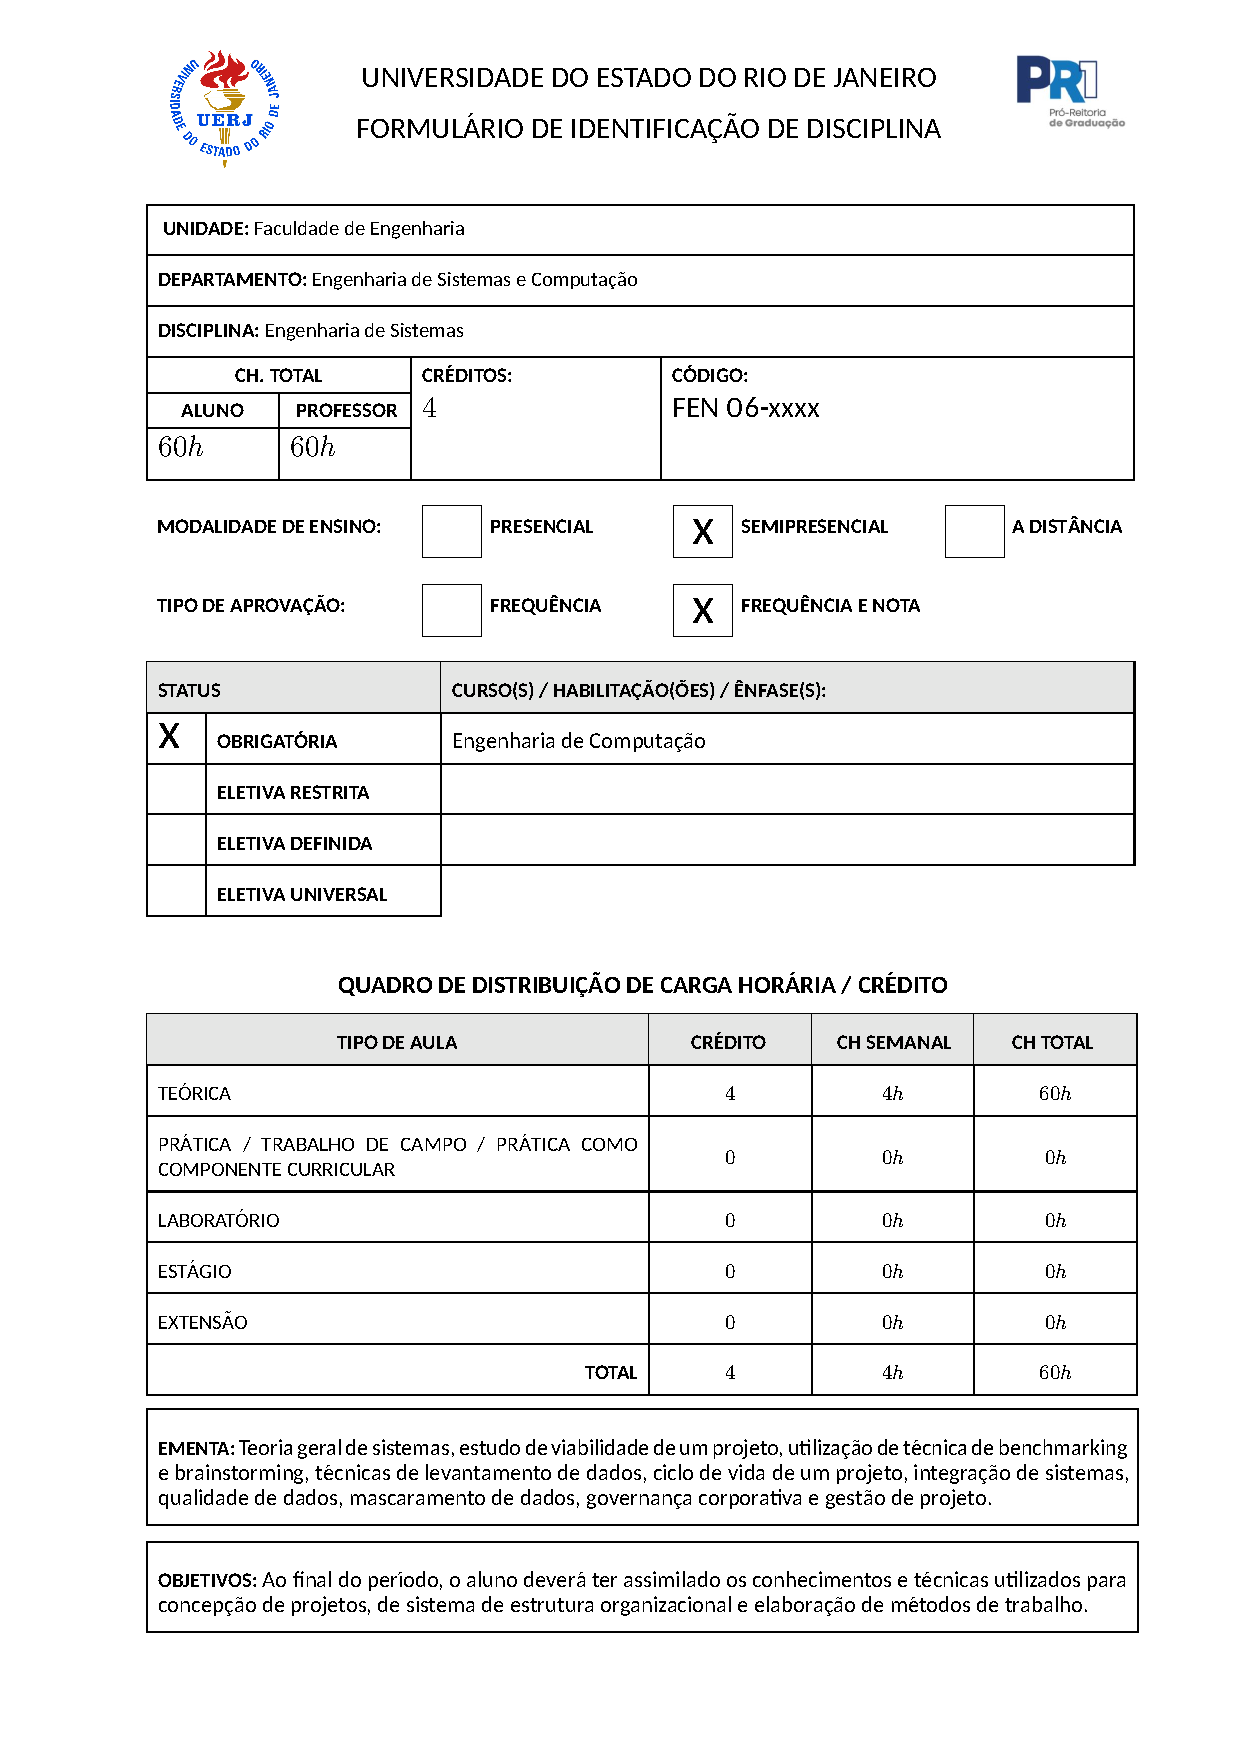
\includepdf[pages=-,addtotoc={1,section,1,{\EngSistA},},pagecommand={\thispagestyle{fancy}}]{ementas/EngenhariaDeSistemas.pdf}
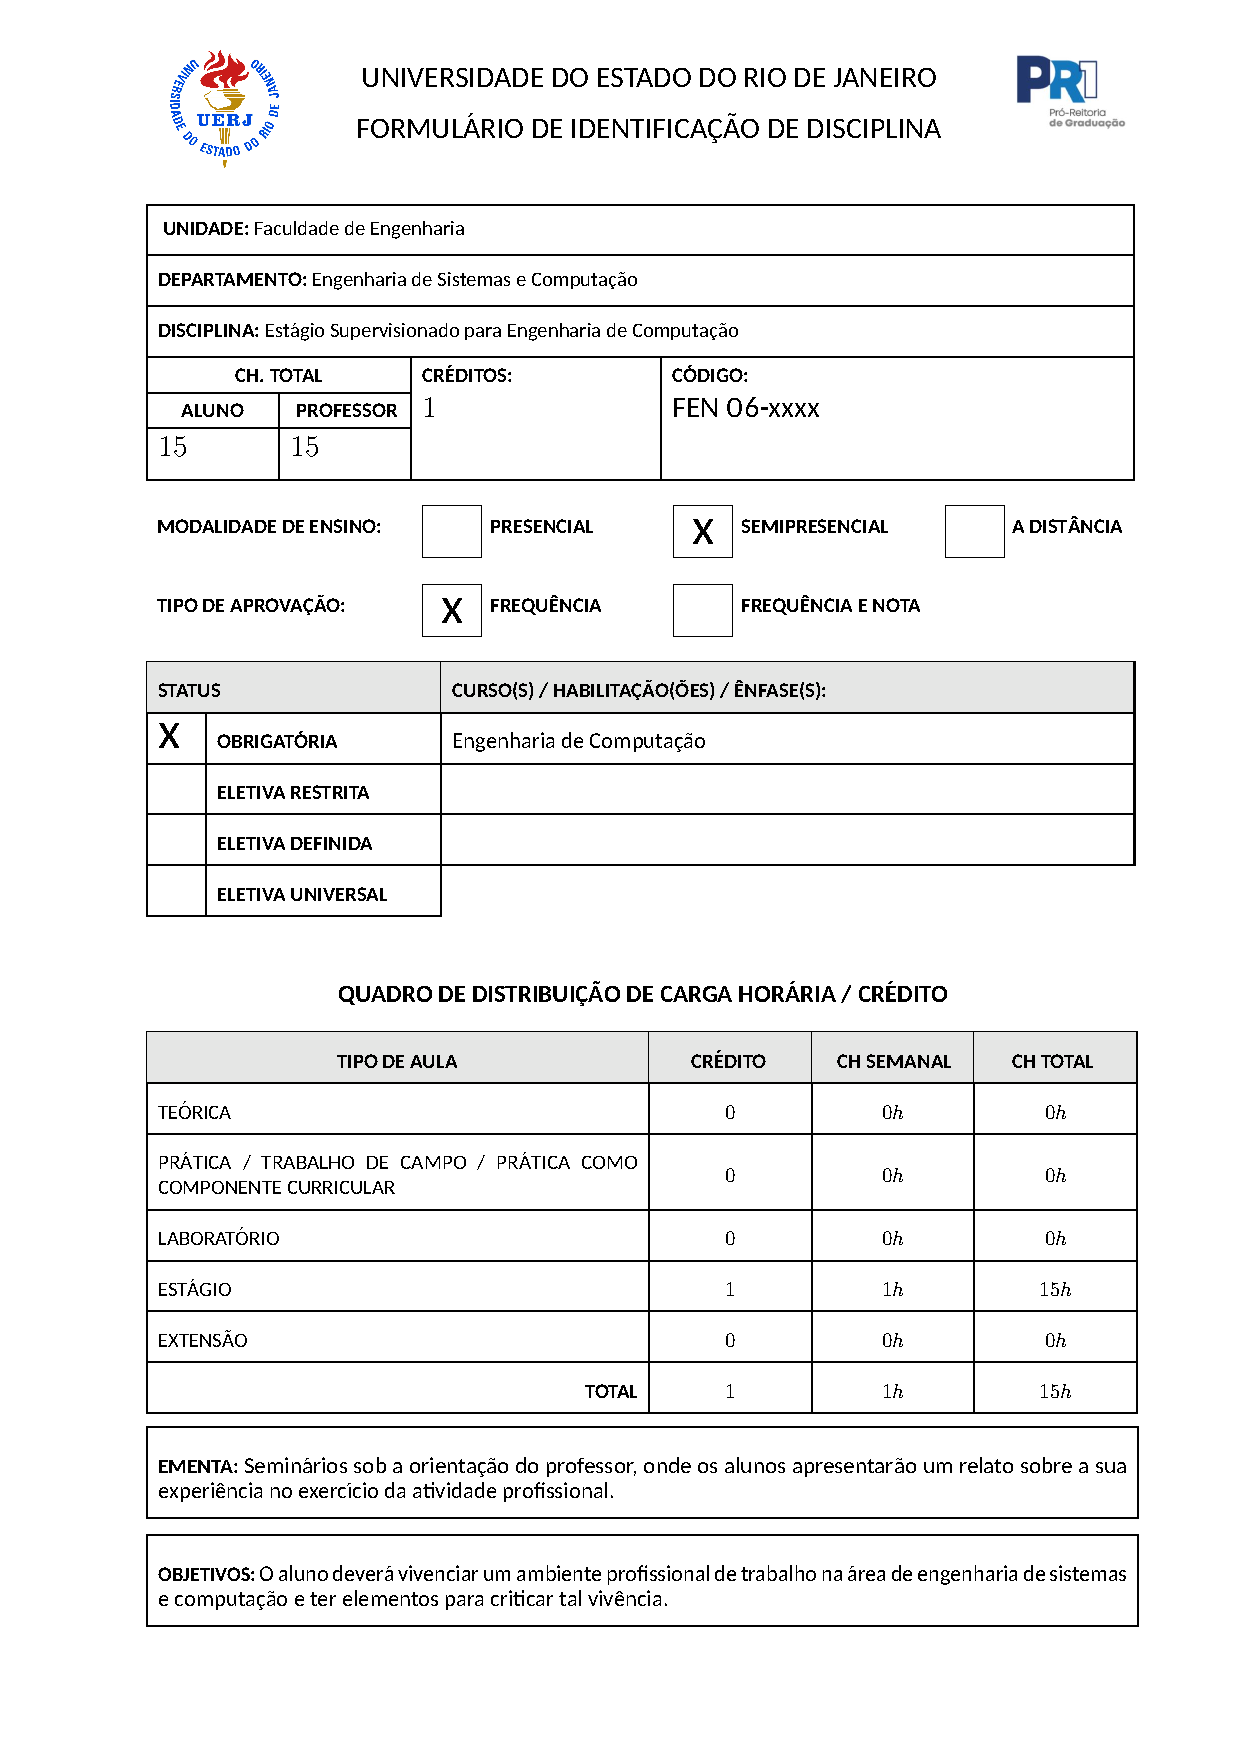
\includepdf[pages=-,addtotoc={1,section,1,{\EstSup},},pagecommand={\thispagestyle{fancy}}]{ementas/EstagioSupervisionadoXIA.pdf}
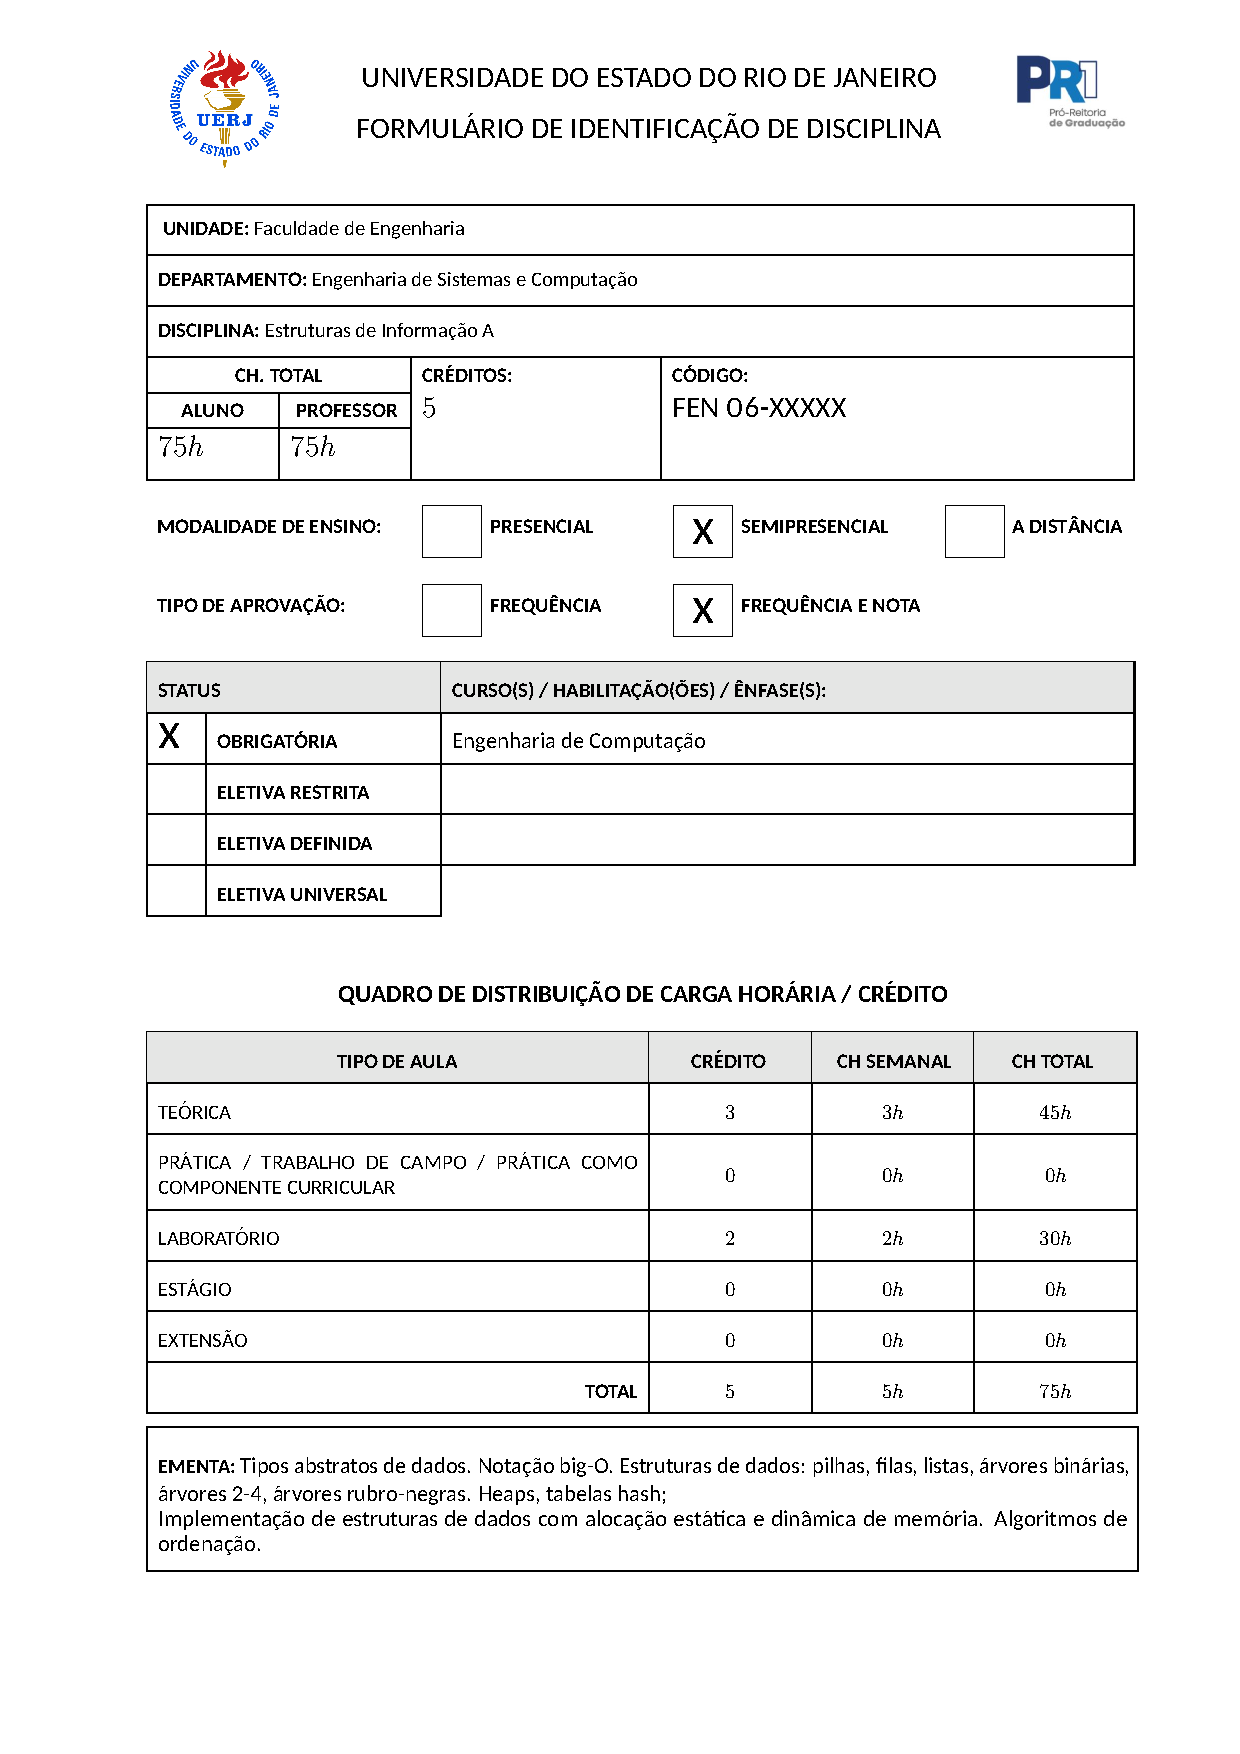
\includepdf[pages=-,addtotoc={1,section,1,{\EstrInf},},pagecommand={\thispagestyle{fancy}}]{ementas/EstruturasDeInformacao.pdf}
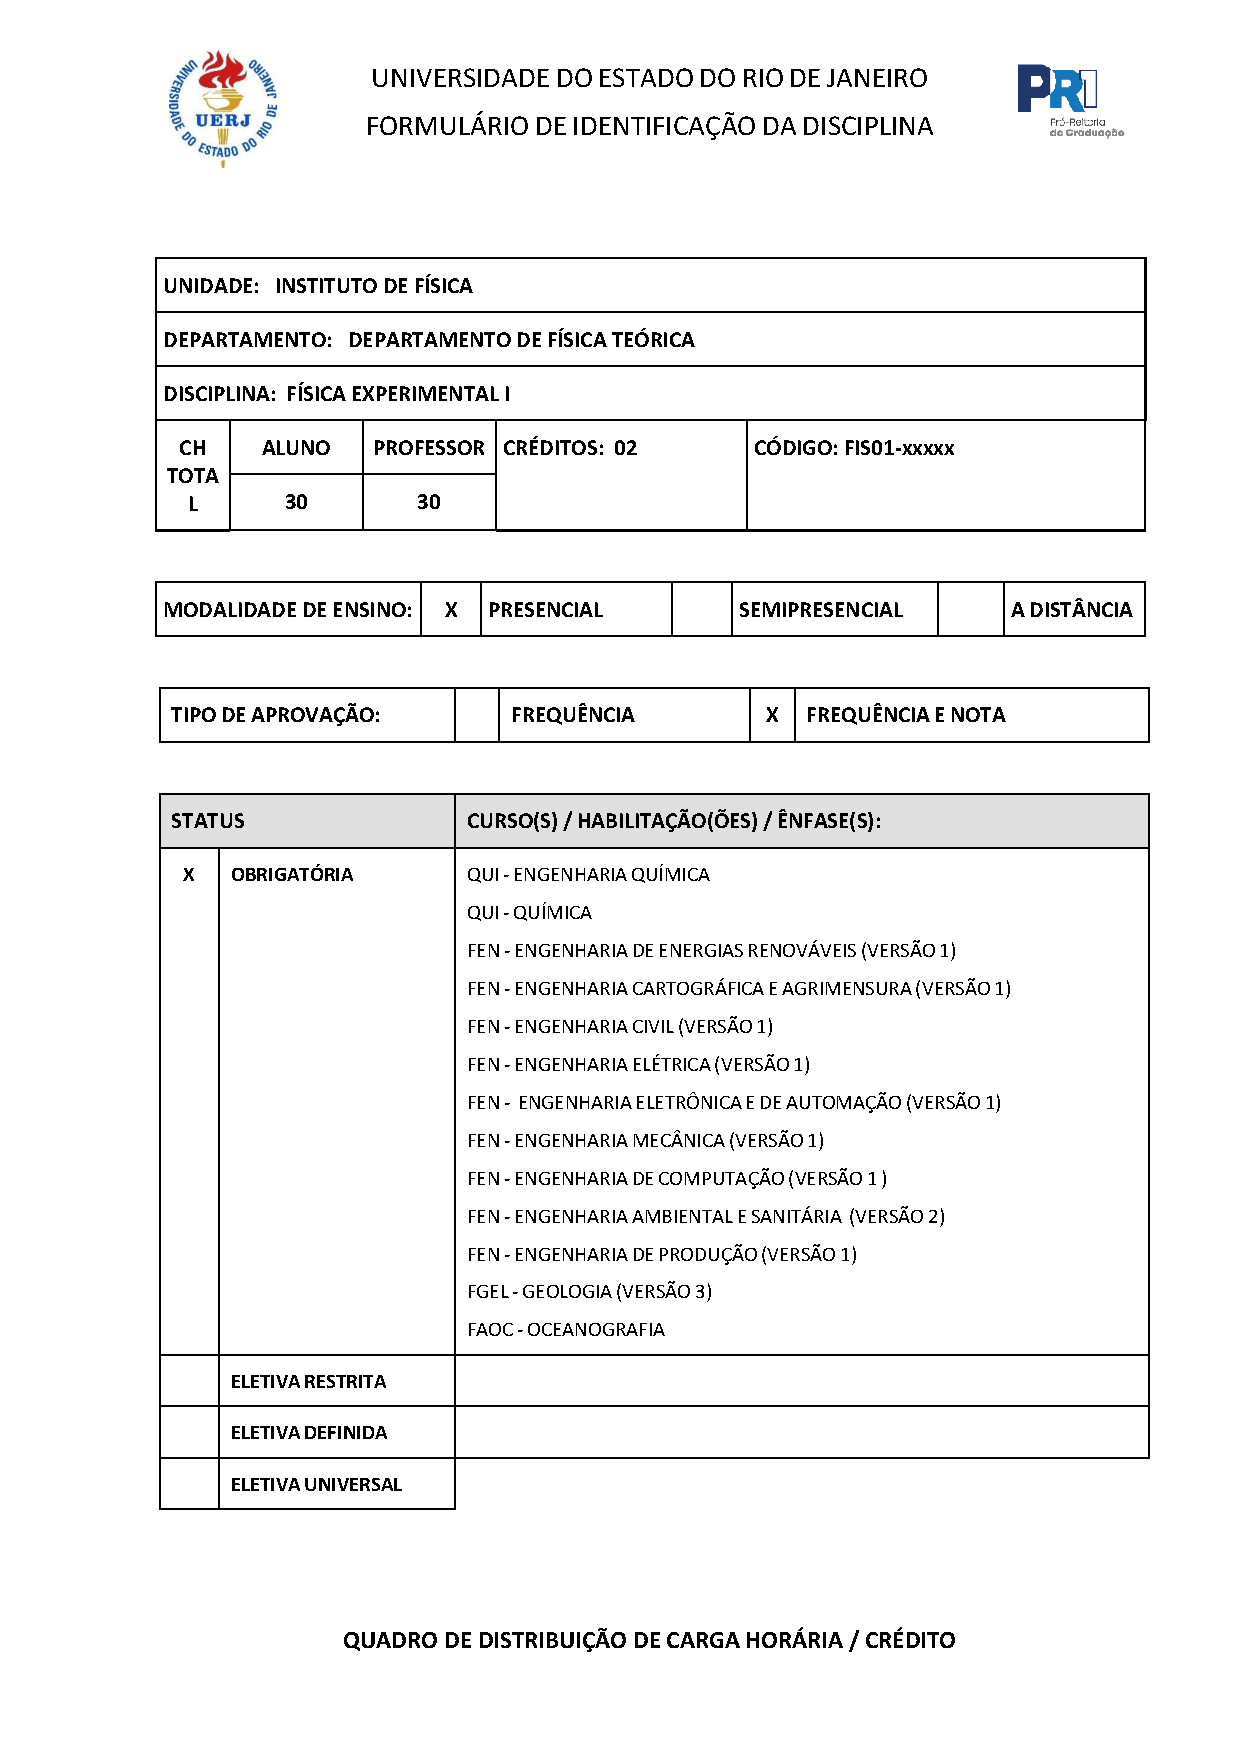
\includepdf[pages=-,addtotoc={1,section,1,{\FisEI},},pagecommand={\thispagestyle{fancy}}]{ementasExternas/FIS01-fisica_experimental_i.pdf}
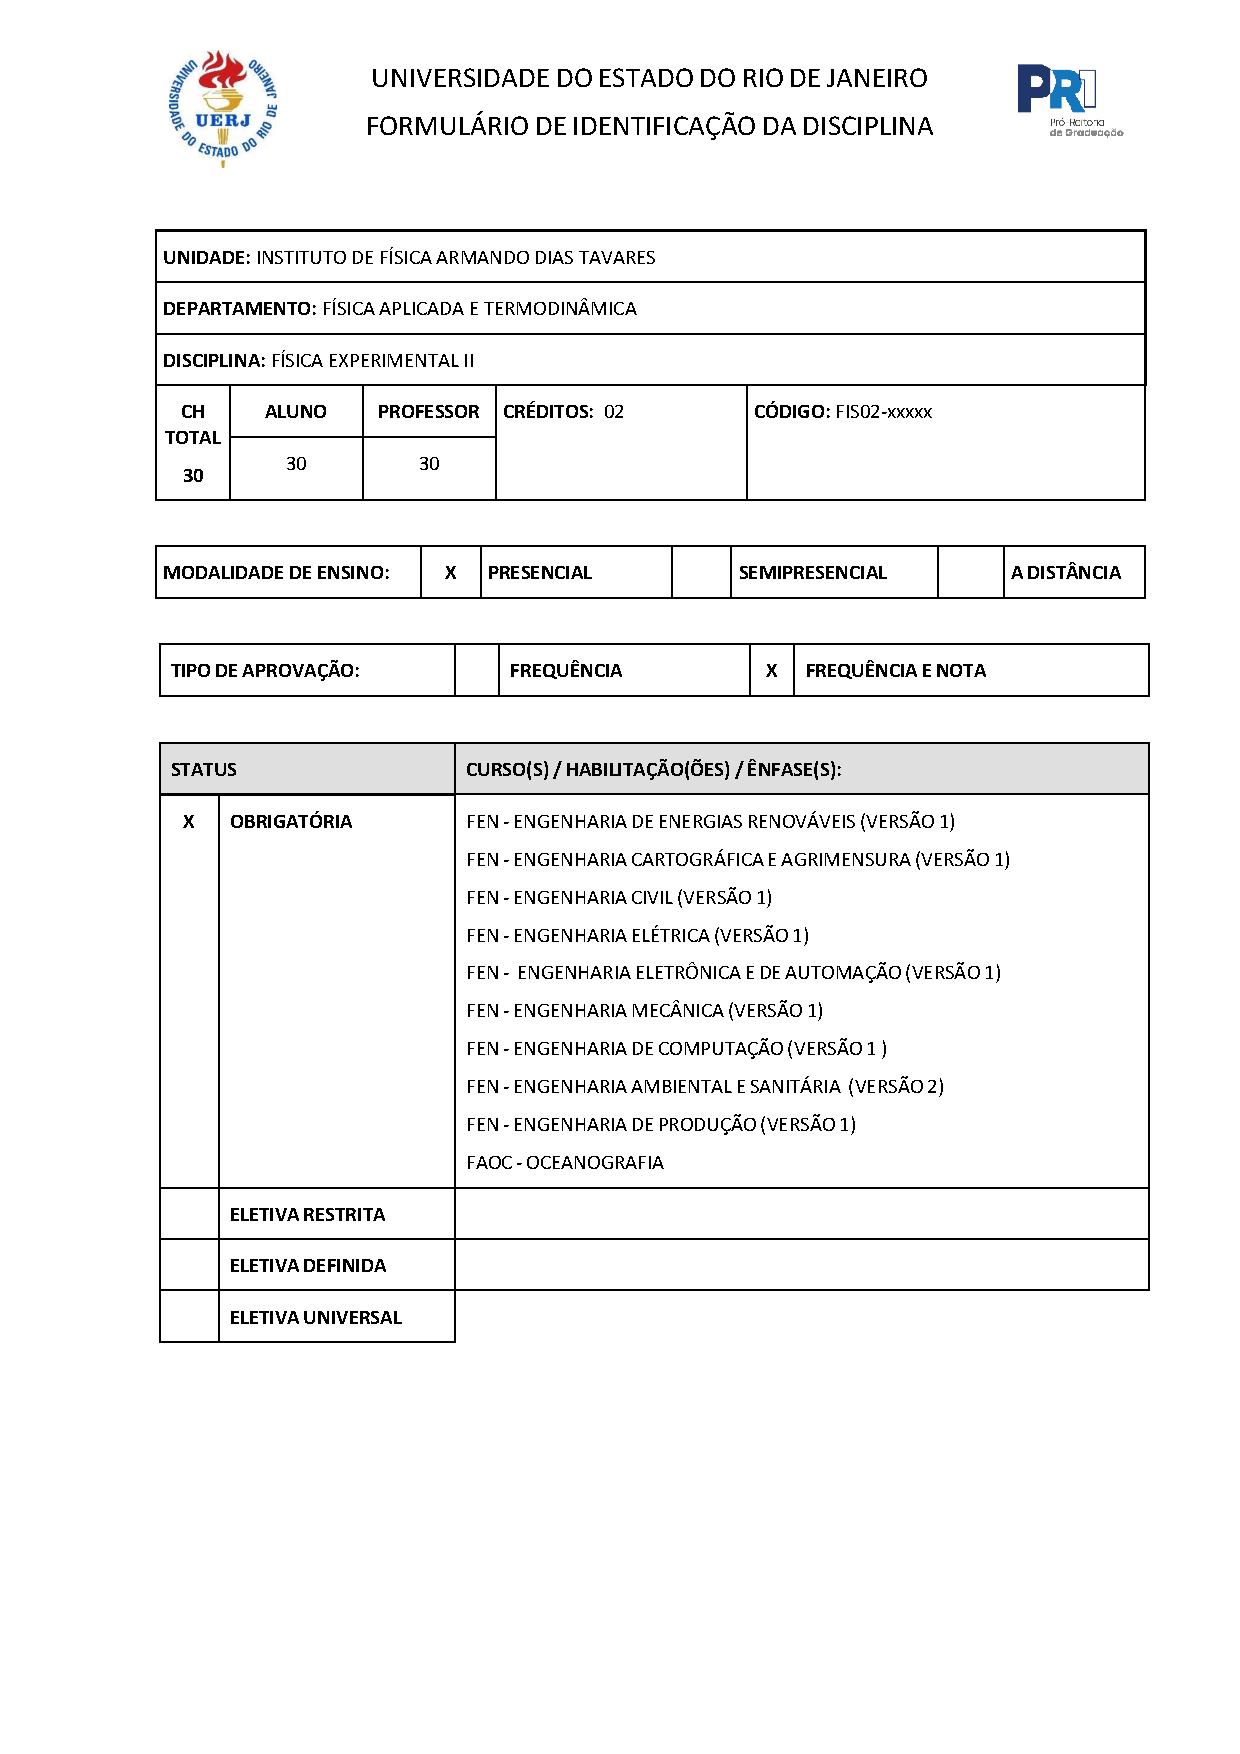
\includepdf[pages=-,addtotoc={1,section,1,{\FisEII},},pagecommand={\thispagestyle{fancy}}]{ementasExternas/FIS02-fisica_experimental_ii.pdf}
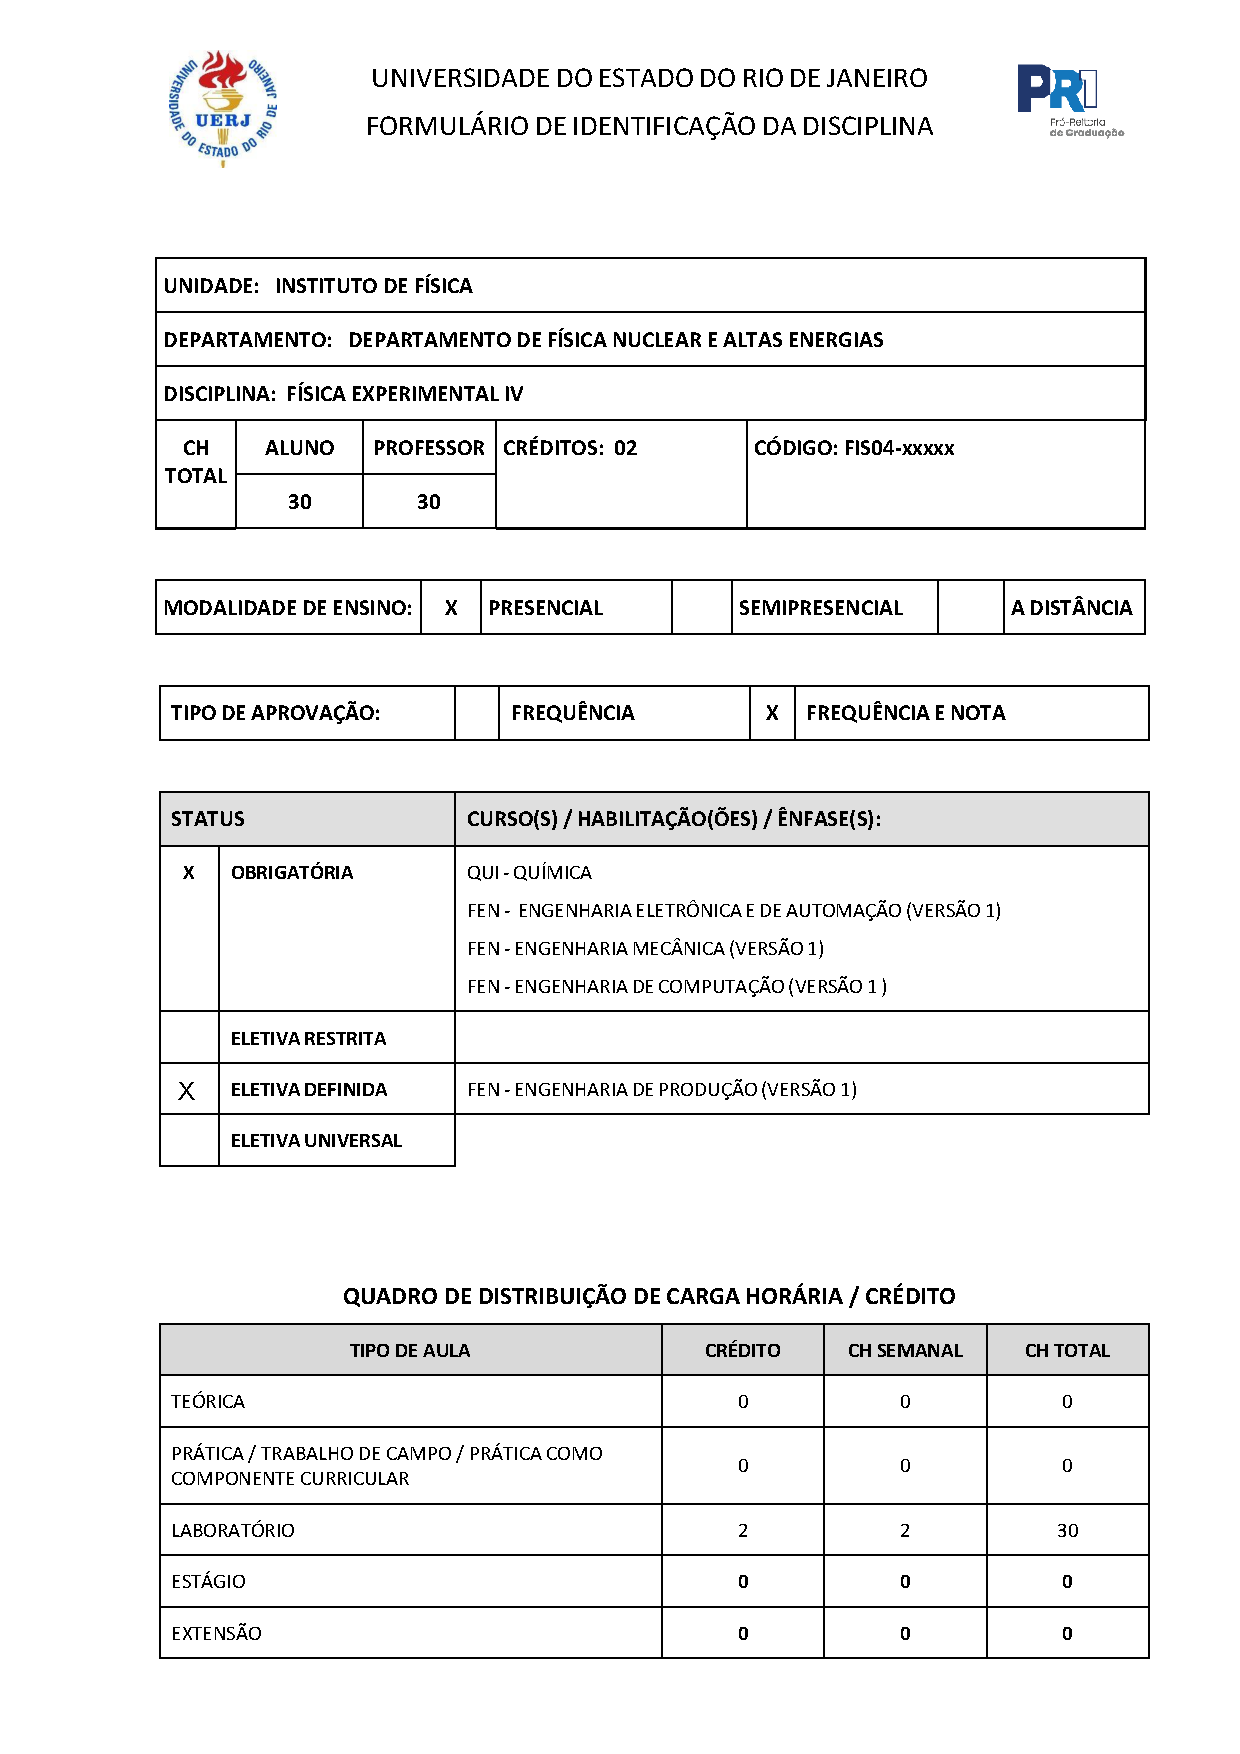
\includepdf[pages=-,addtotoc={1,section,1,{\FisEIV},},pagecommand={\thispagestyle{fancy}}]{ementasExternas/FIS04-fisica_experimental_iv.pdf}
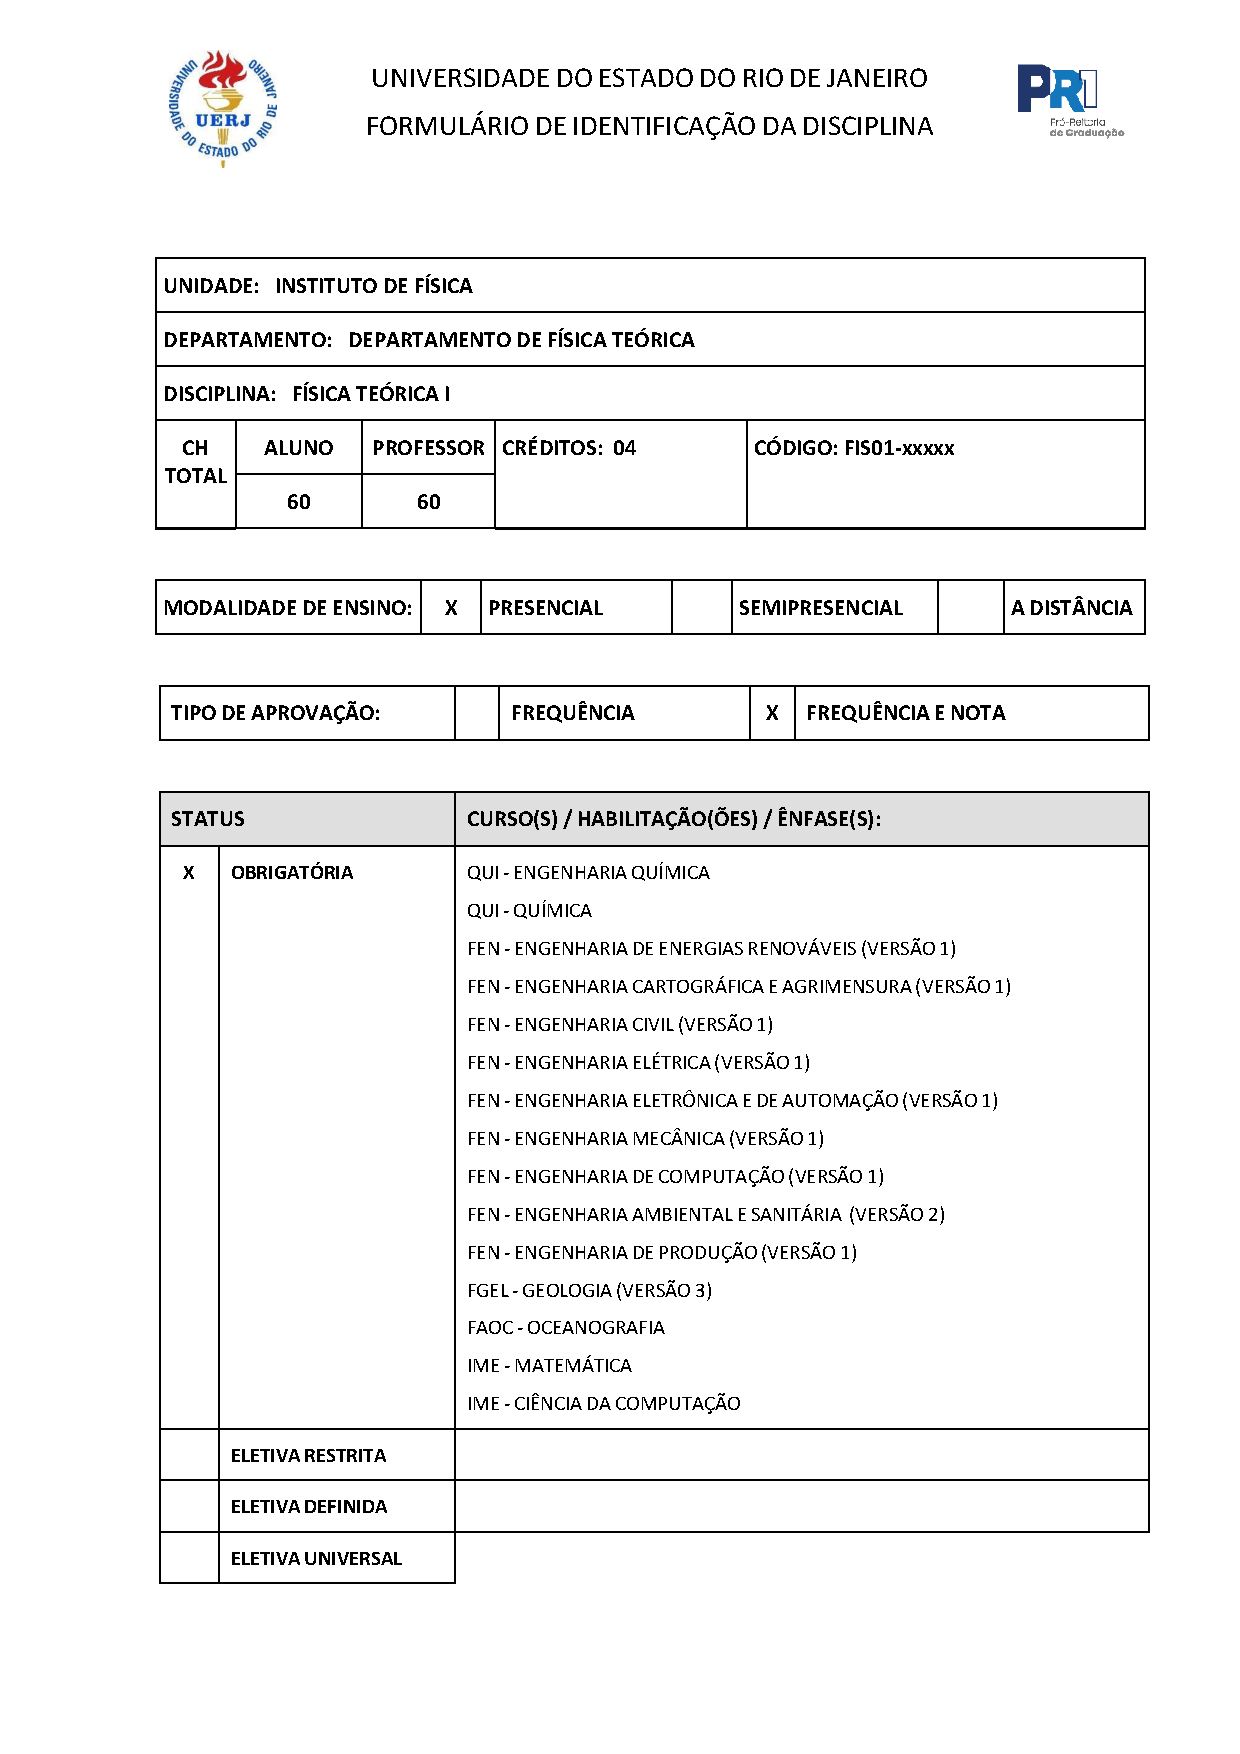
\includepdf[pages=-,addtotoc={1,section,1,{\FisI},},pagecommand={\thispagestyle{fancy}}]{ementasExternas/FIS01-fisica_teorica_i.pdf}
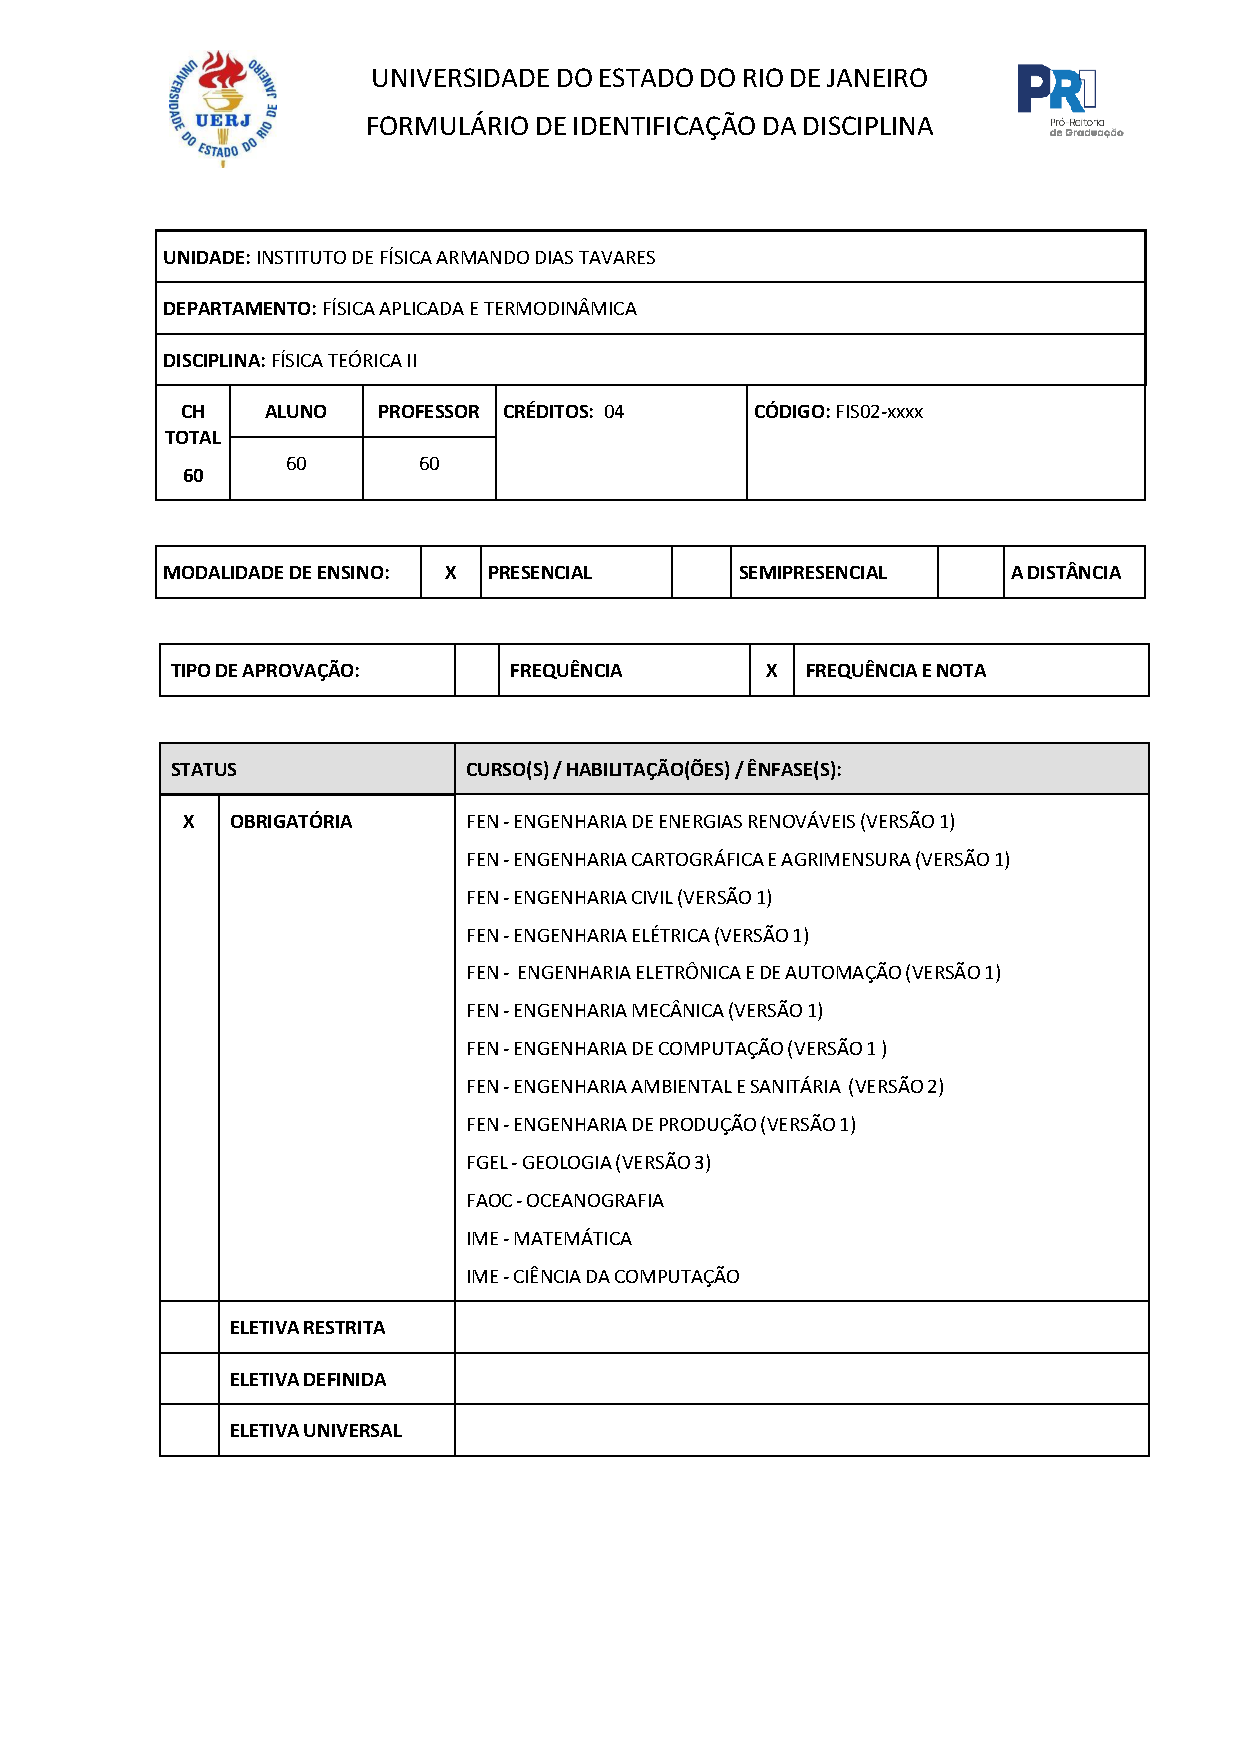
\includepdf[pages=-,addtotoc={1,section,1,{\FisII},},pagecommand={\thispagestyle{fancy}}]{ementasExternas/FIS02-fisica_teorica_ii.pdf}
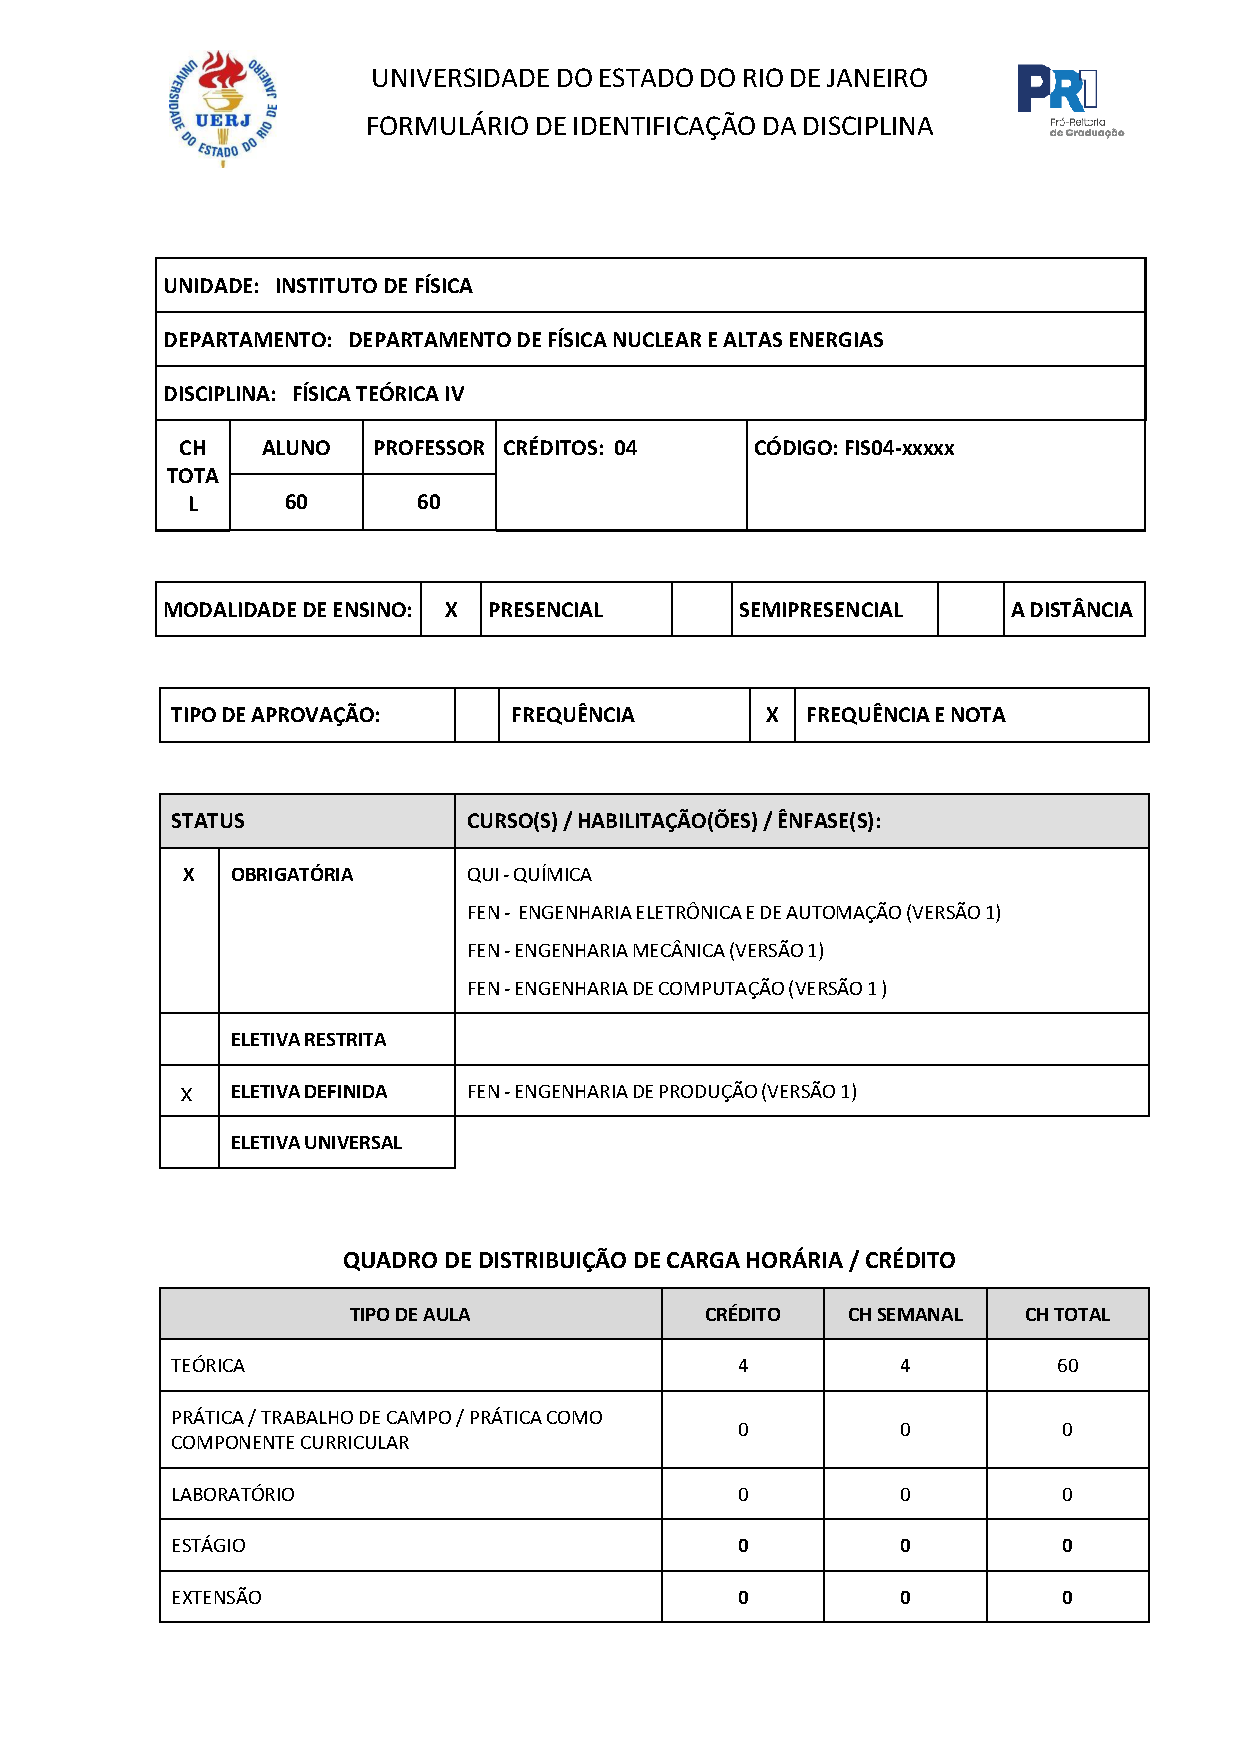
\includepdf[pages=-,addtotoc={1,section,1,{\FisIV},},pagecommand={\thispagestyle{fancy}}]{ementasExternas/FIS04-fisica_teorica_iv.pdf}
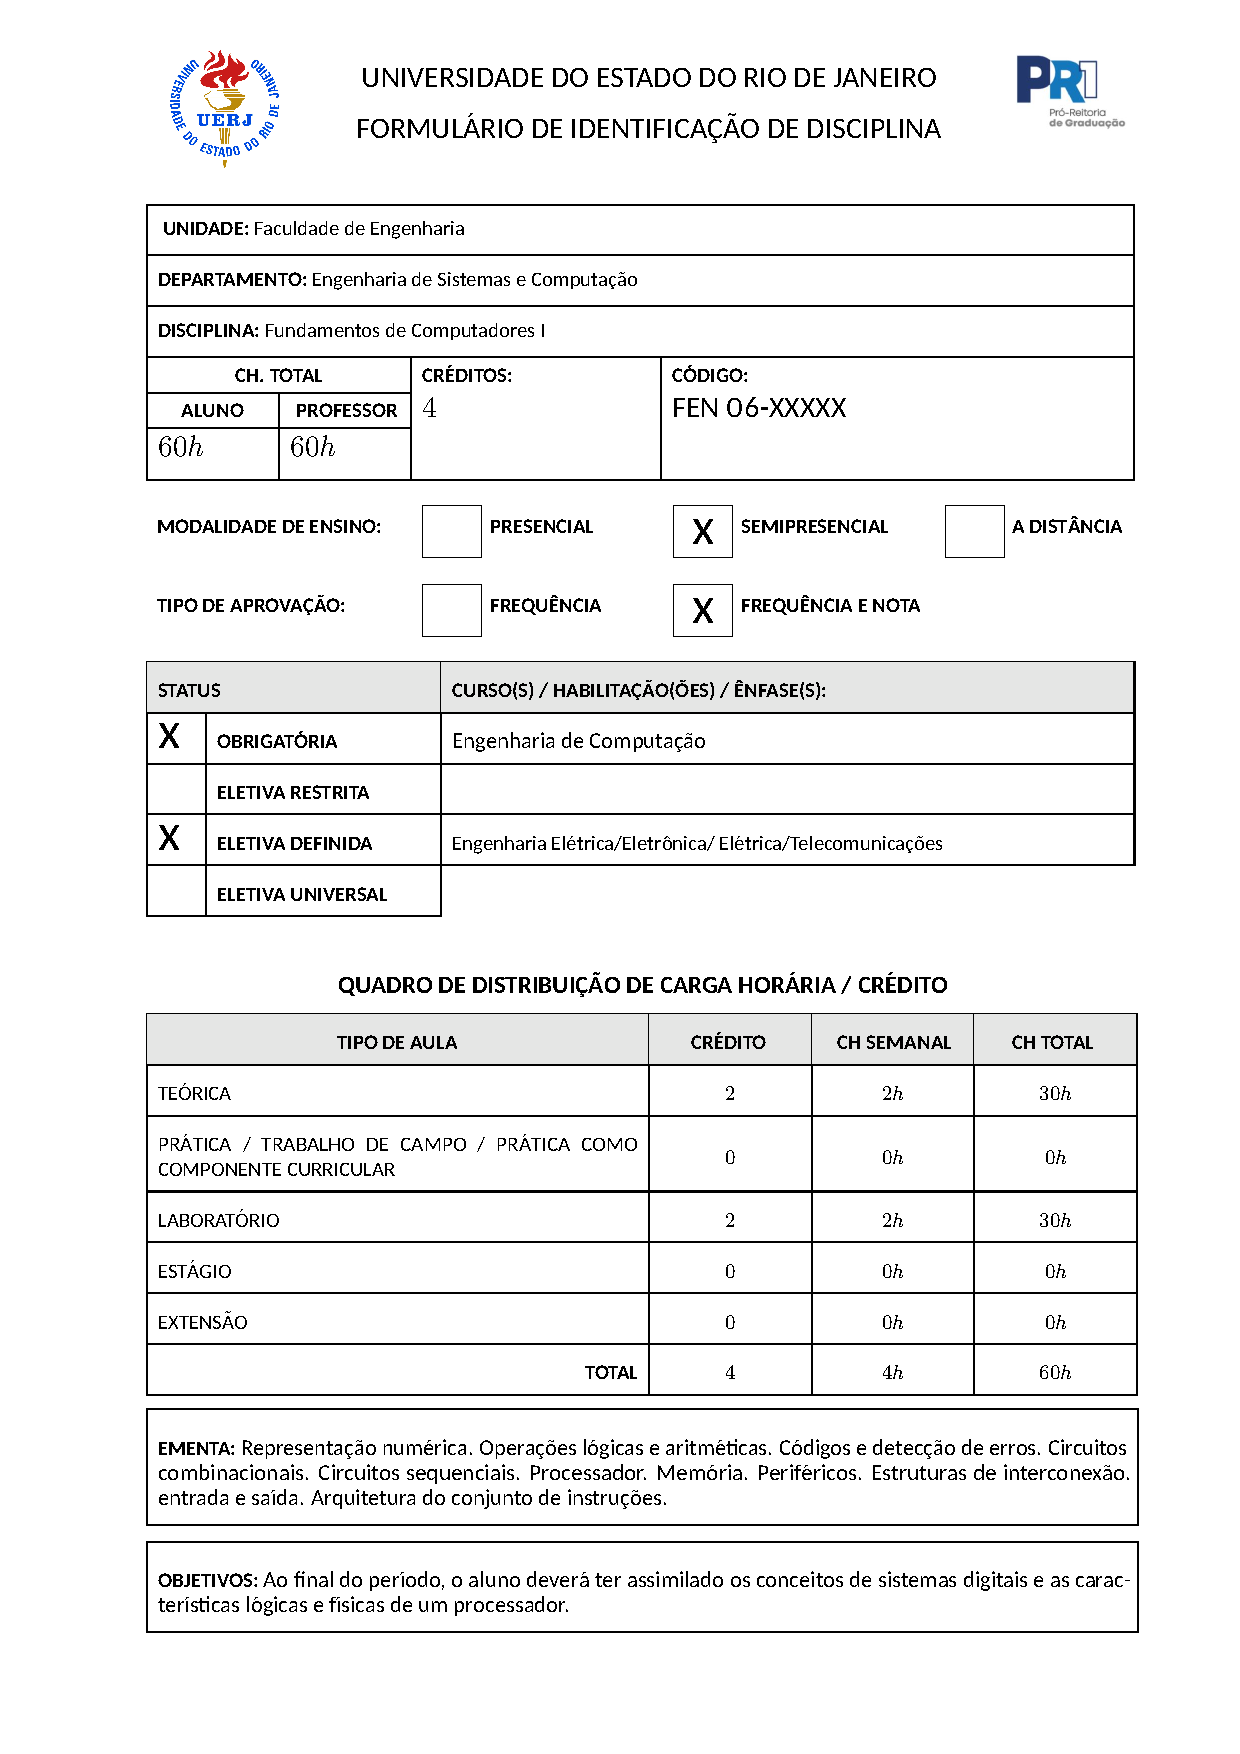
\includepdf[pages=-,addtotoc={1,section,1,{\FundComp},},pagecommand={\thispagestyle{fancy}}]{ementas/FundamentosDeComputadores.pdf}
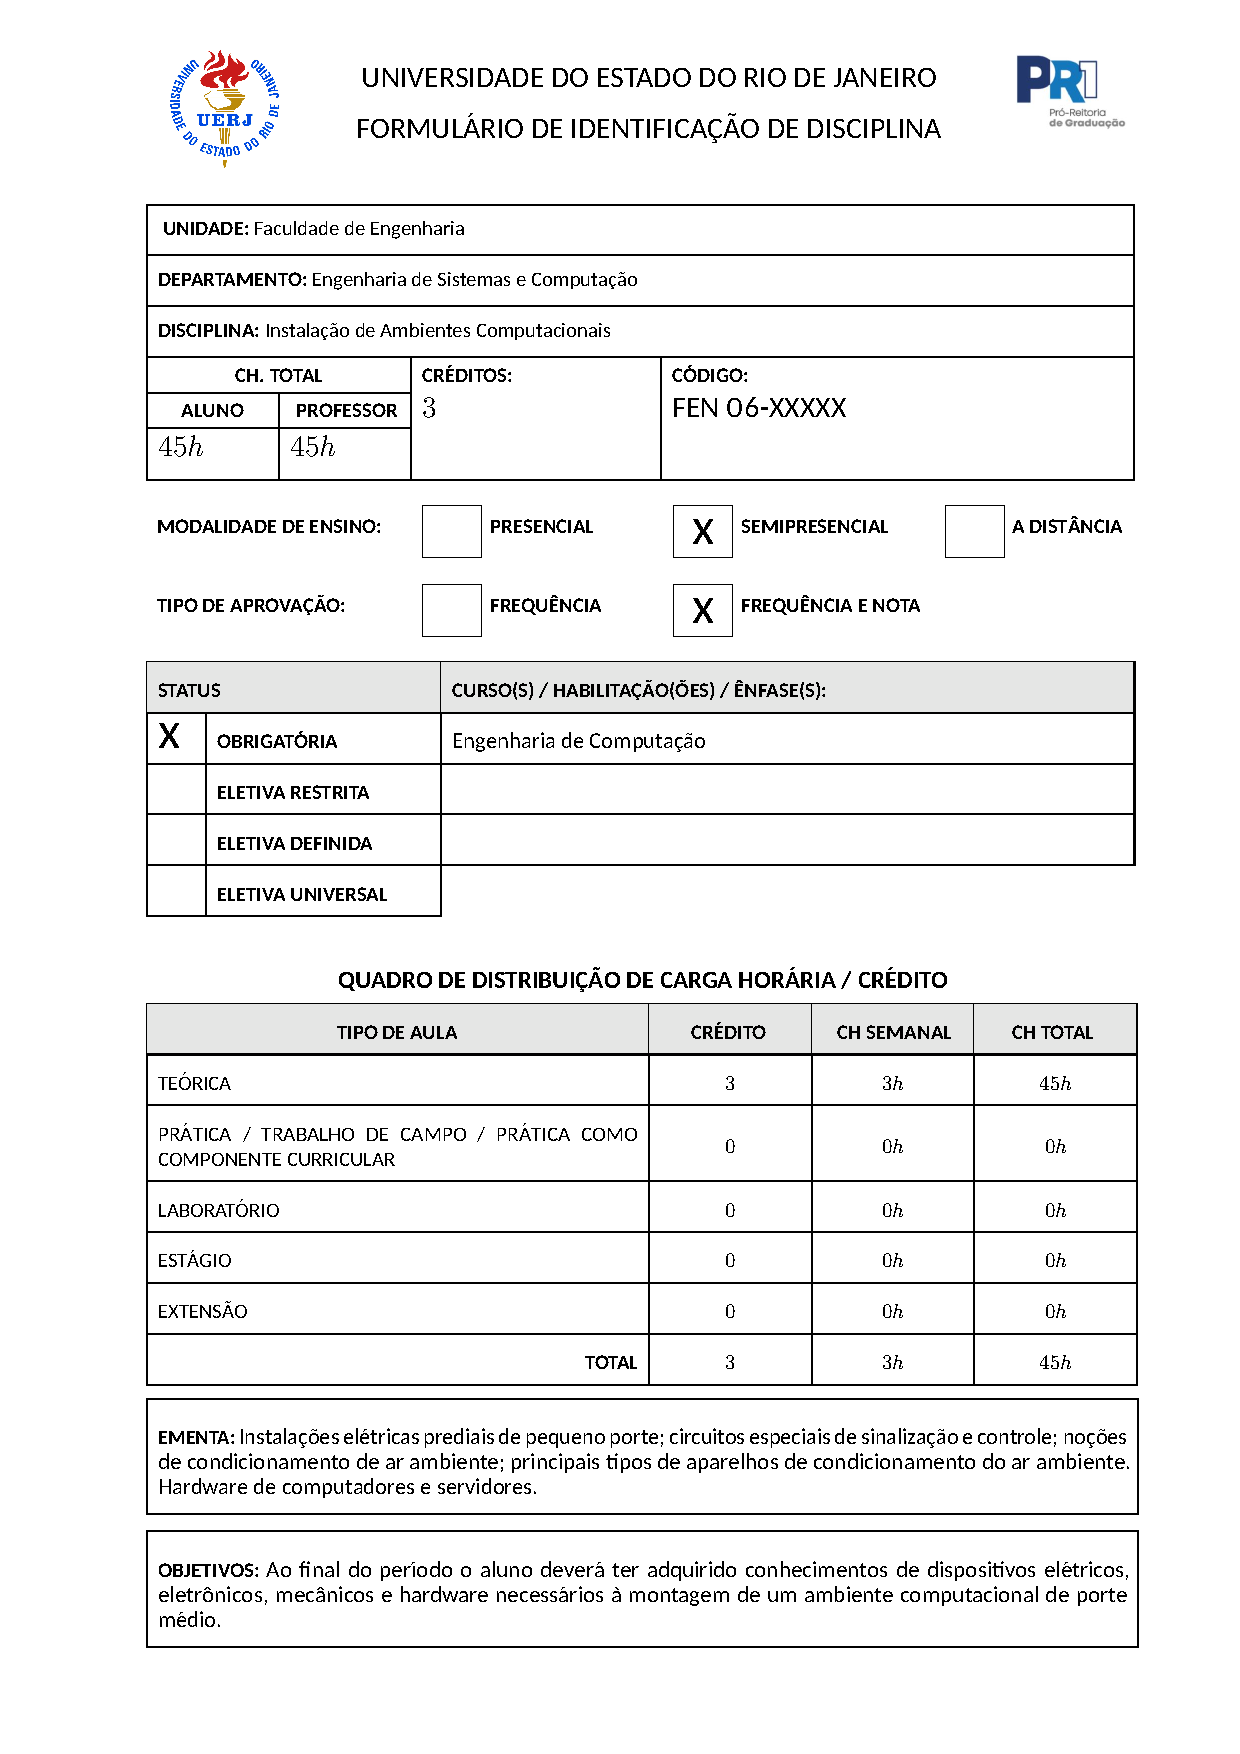
\includepdf[pages=-,addtotoc={1,section,1,{\Instala},},pagecommand={\thispagestyle{fancy}}]{ementas/instalacao_de_ambientes_computacionais.pdf}
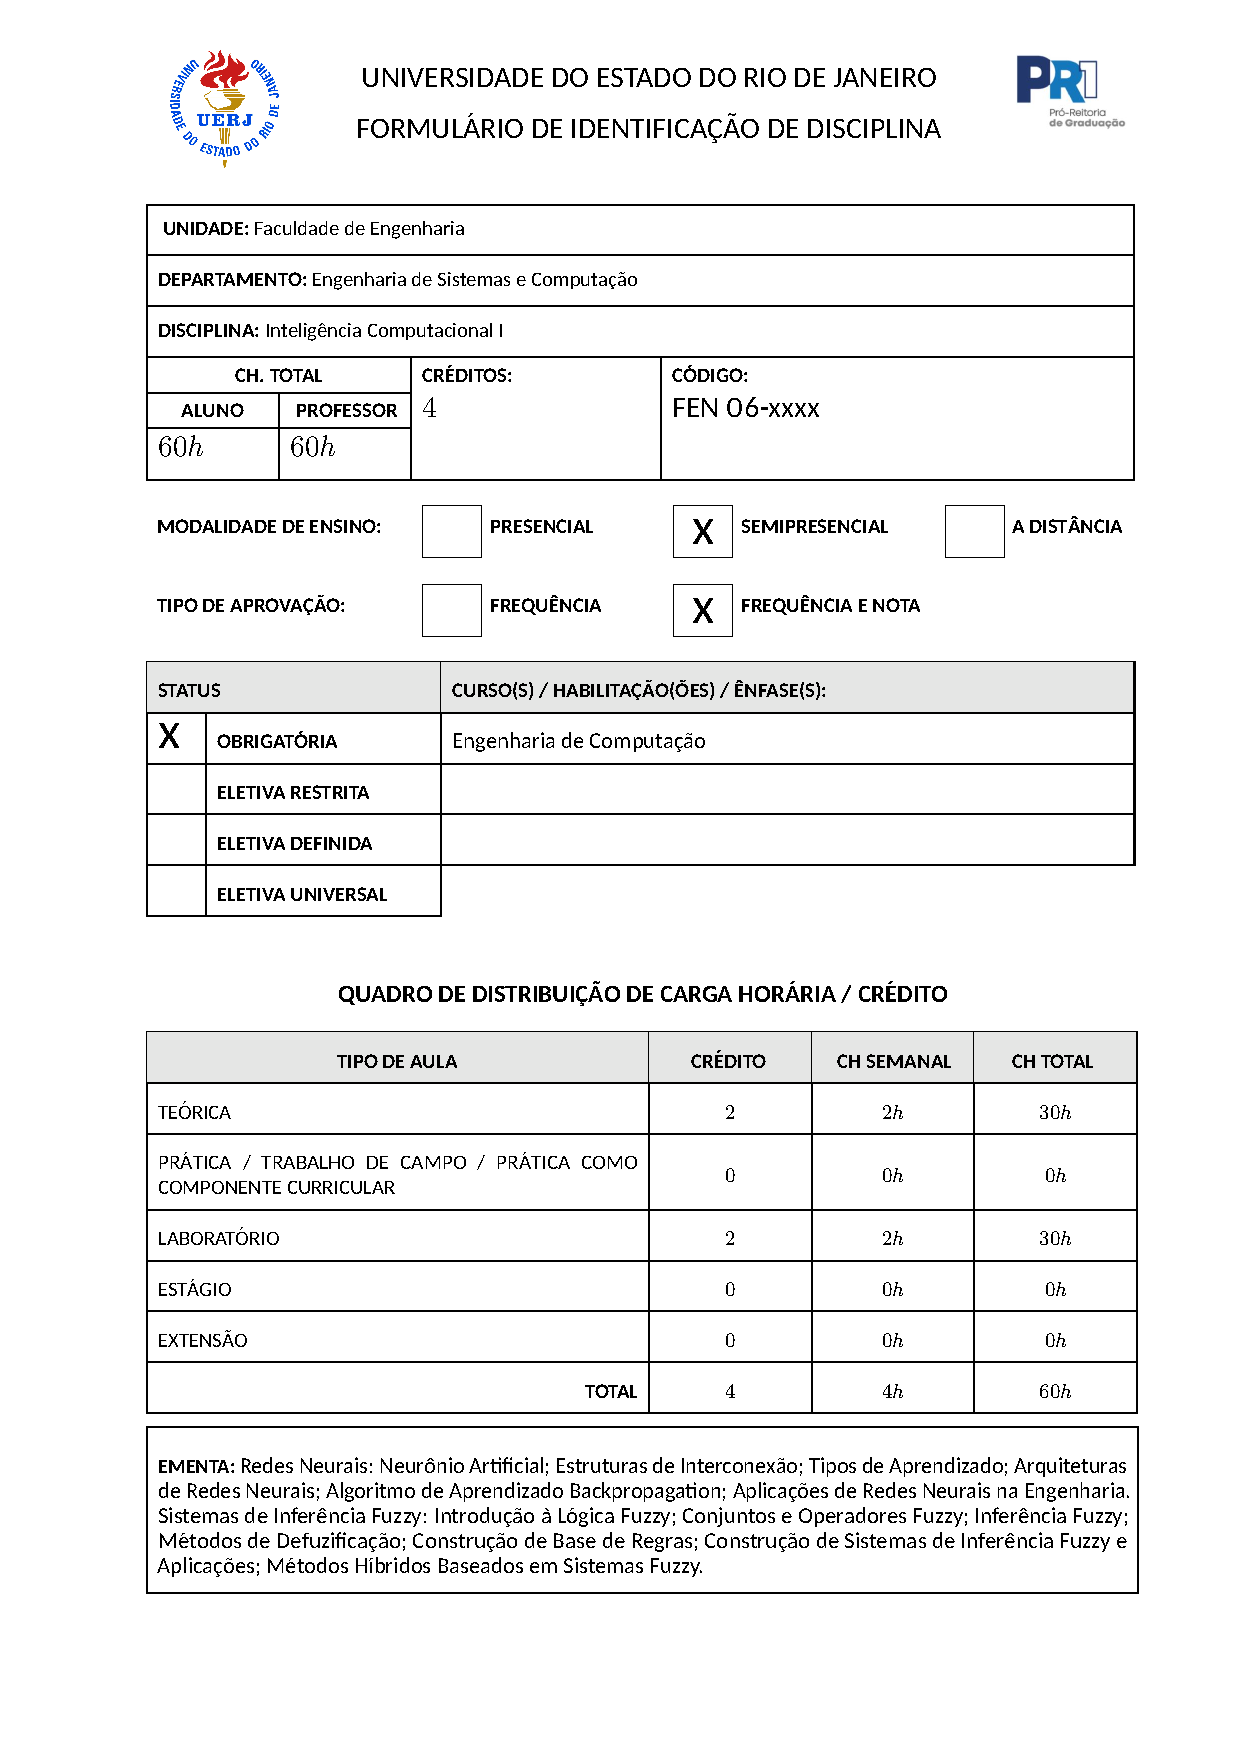
\includepdf[pages=-,addtotoc={1,section,1,{\IC},},pagecommand={\thispagestyle{fancy}}]{ementas/InteligenciaComputacional1.pdf}
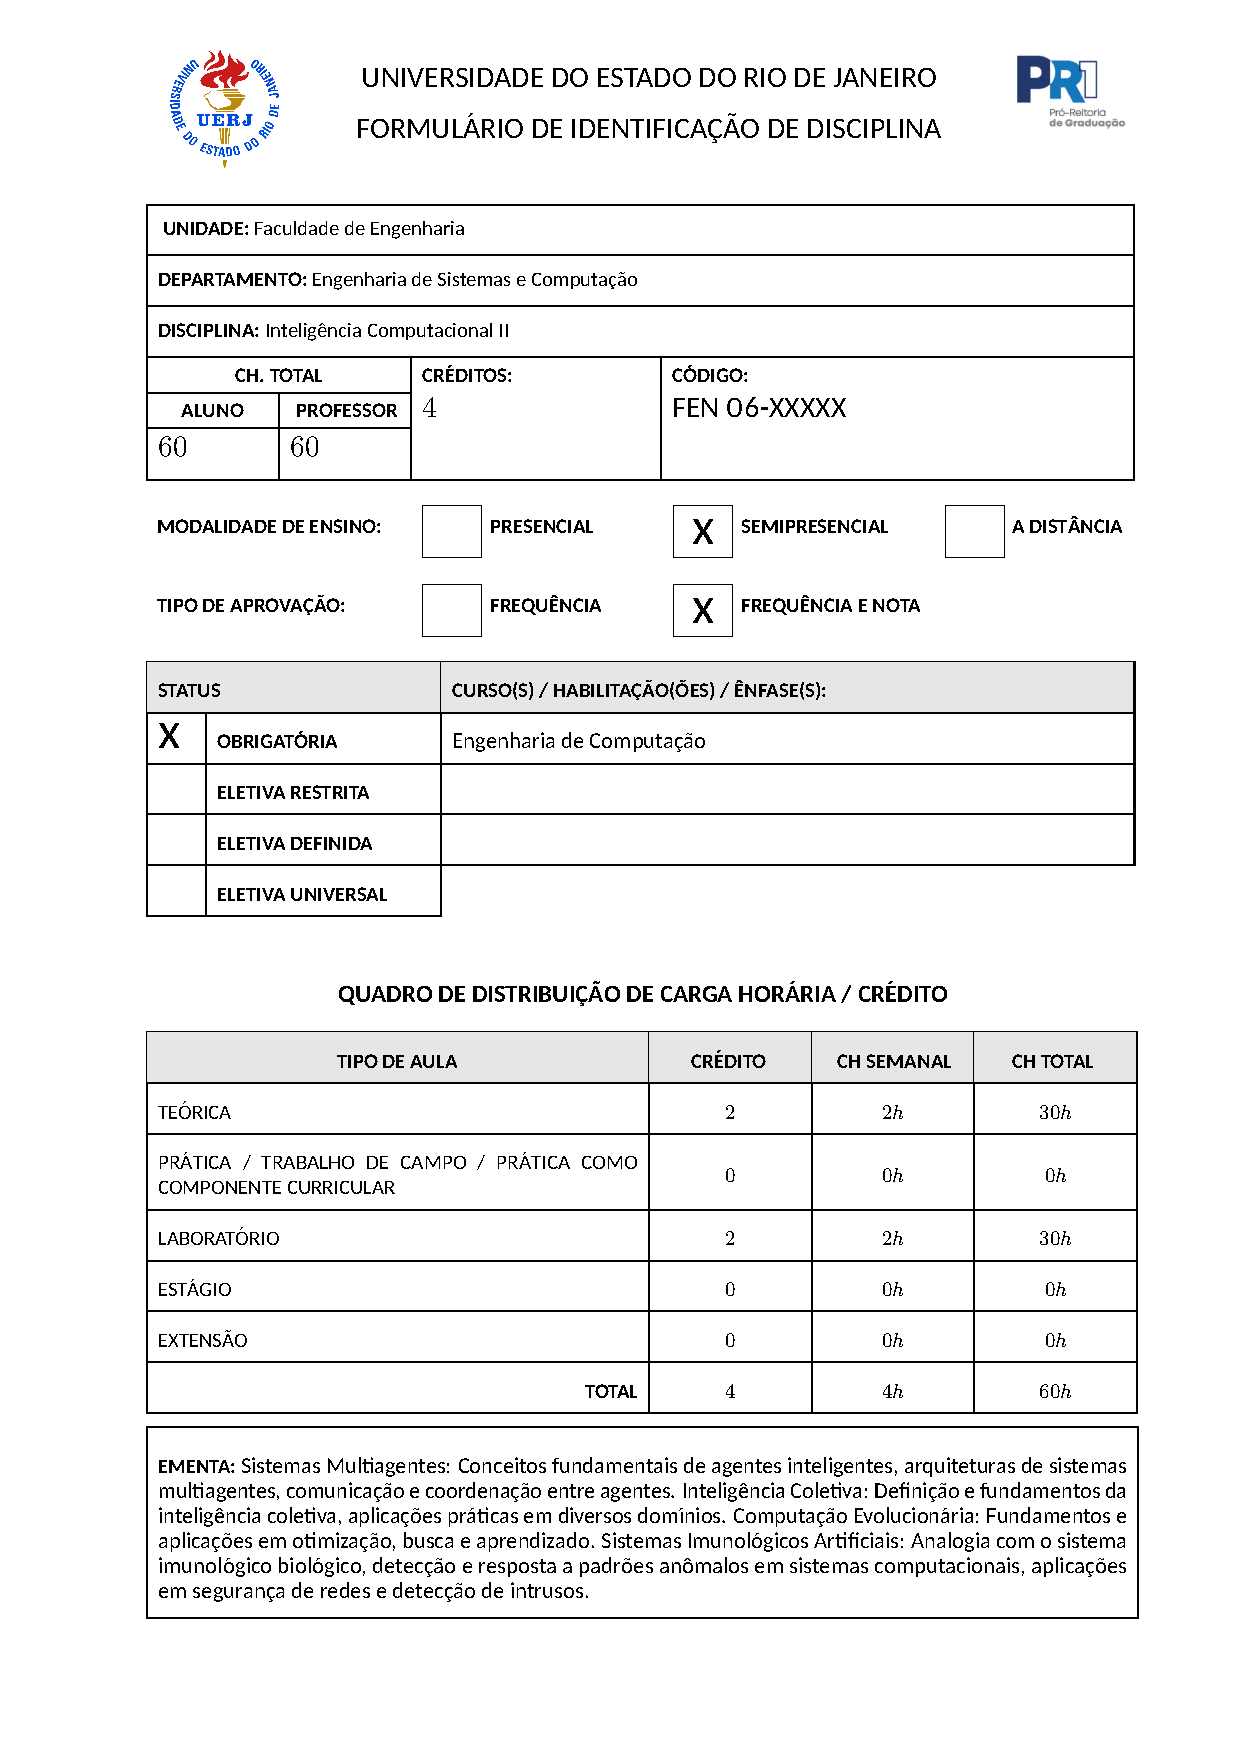
\includepdf[pages=-,addtotoc={1,section,1,{\ICII},},pagecommand={\thispagestyle{fancy}}]{ementas/InteligenciaComputacional2.pdf}
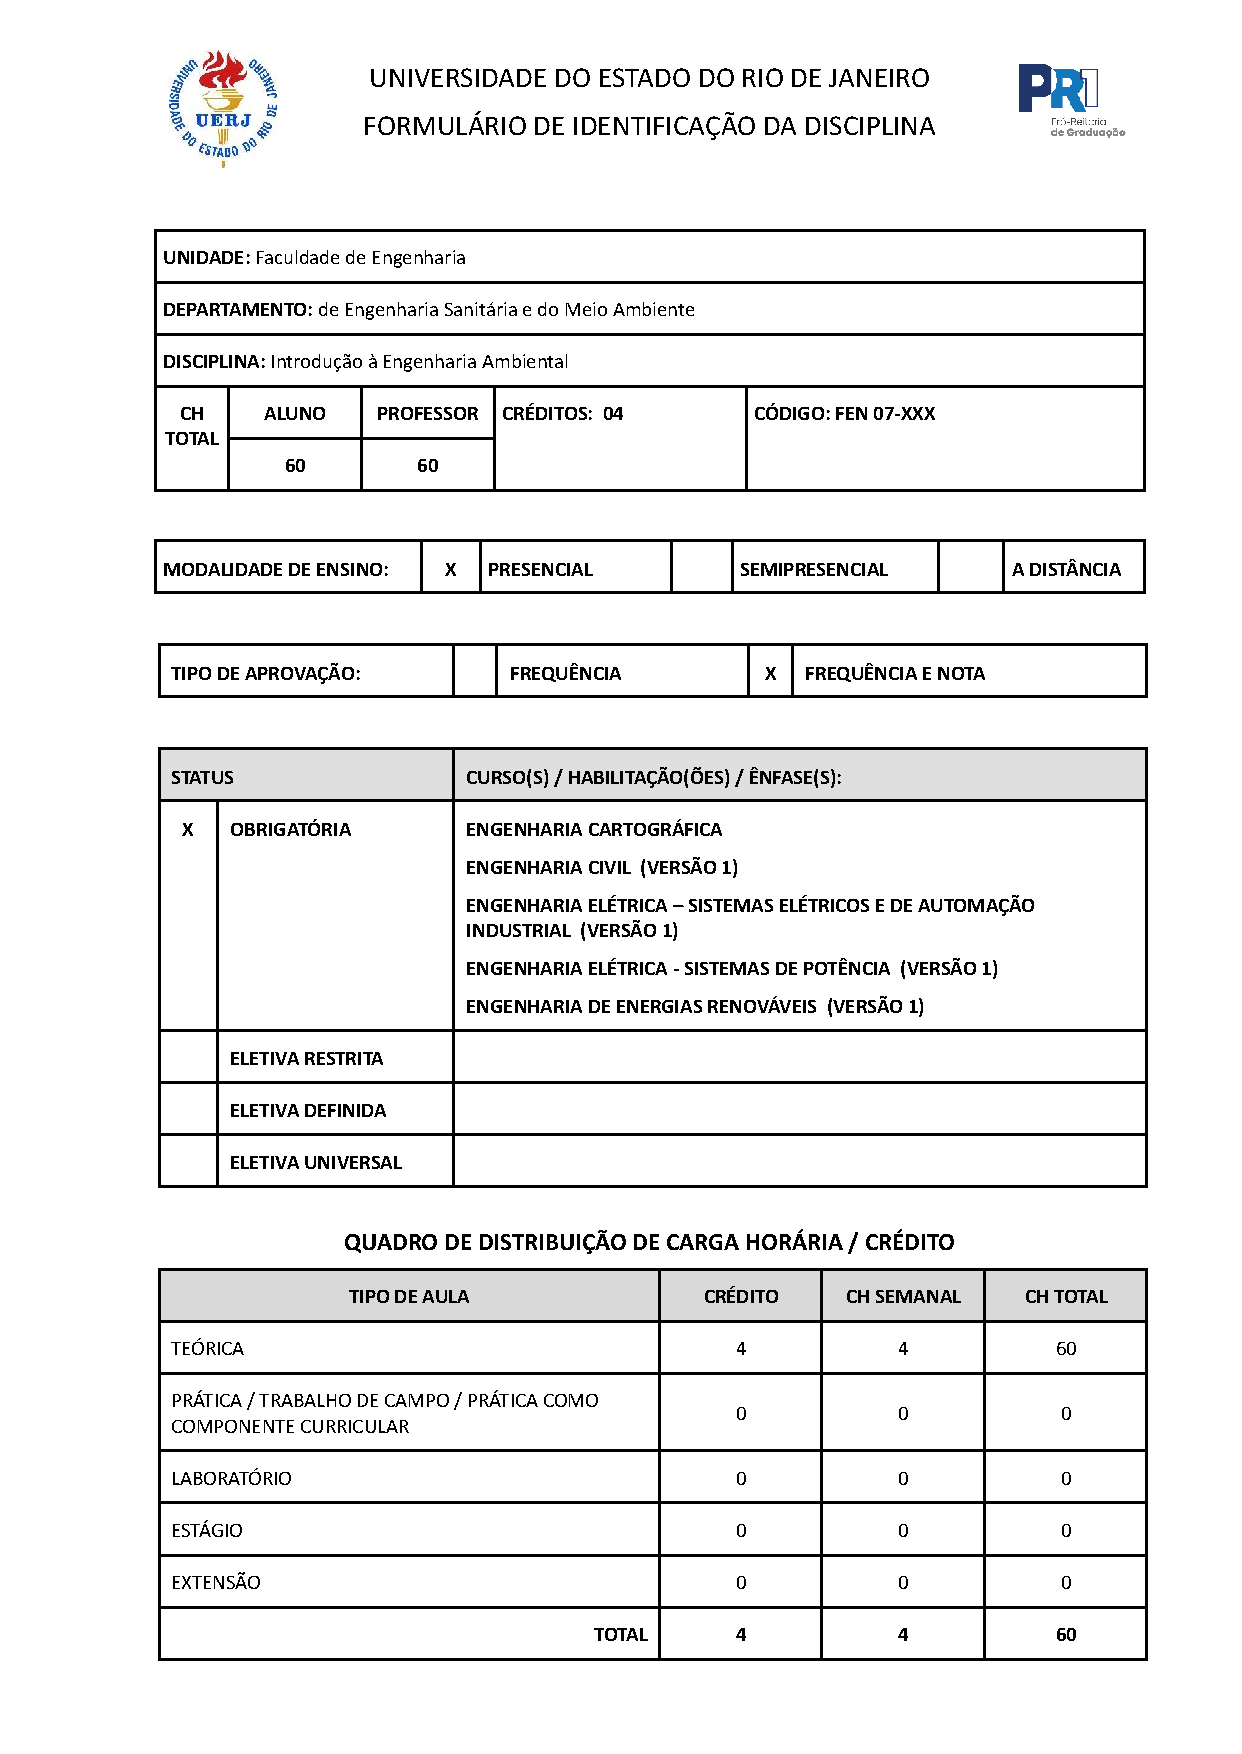
\includepdf[pages=-,addtotoc={1,section,1,{\IntAmb},},pagecommand={\thispagestyle{fancy}}]{ementasExternas/Introducao_a_Engenharia_Ambiental.pdf}
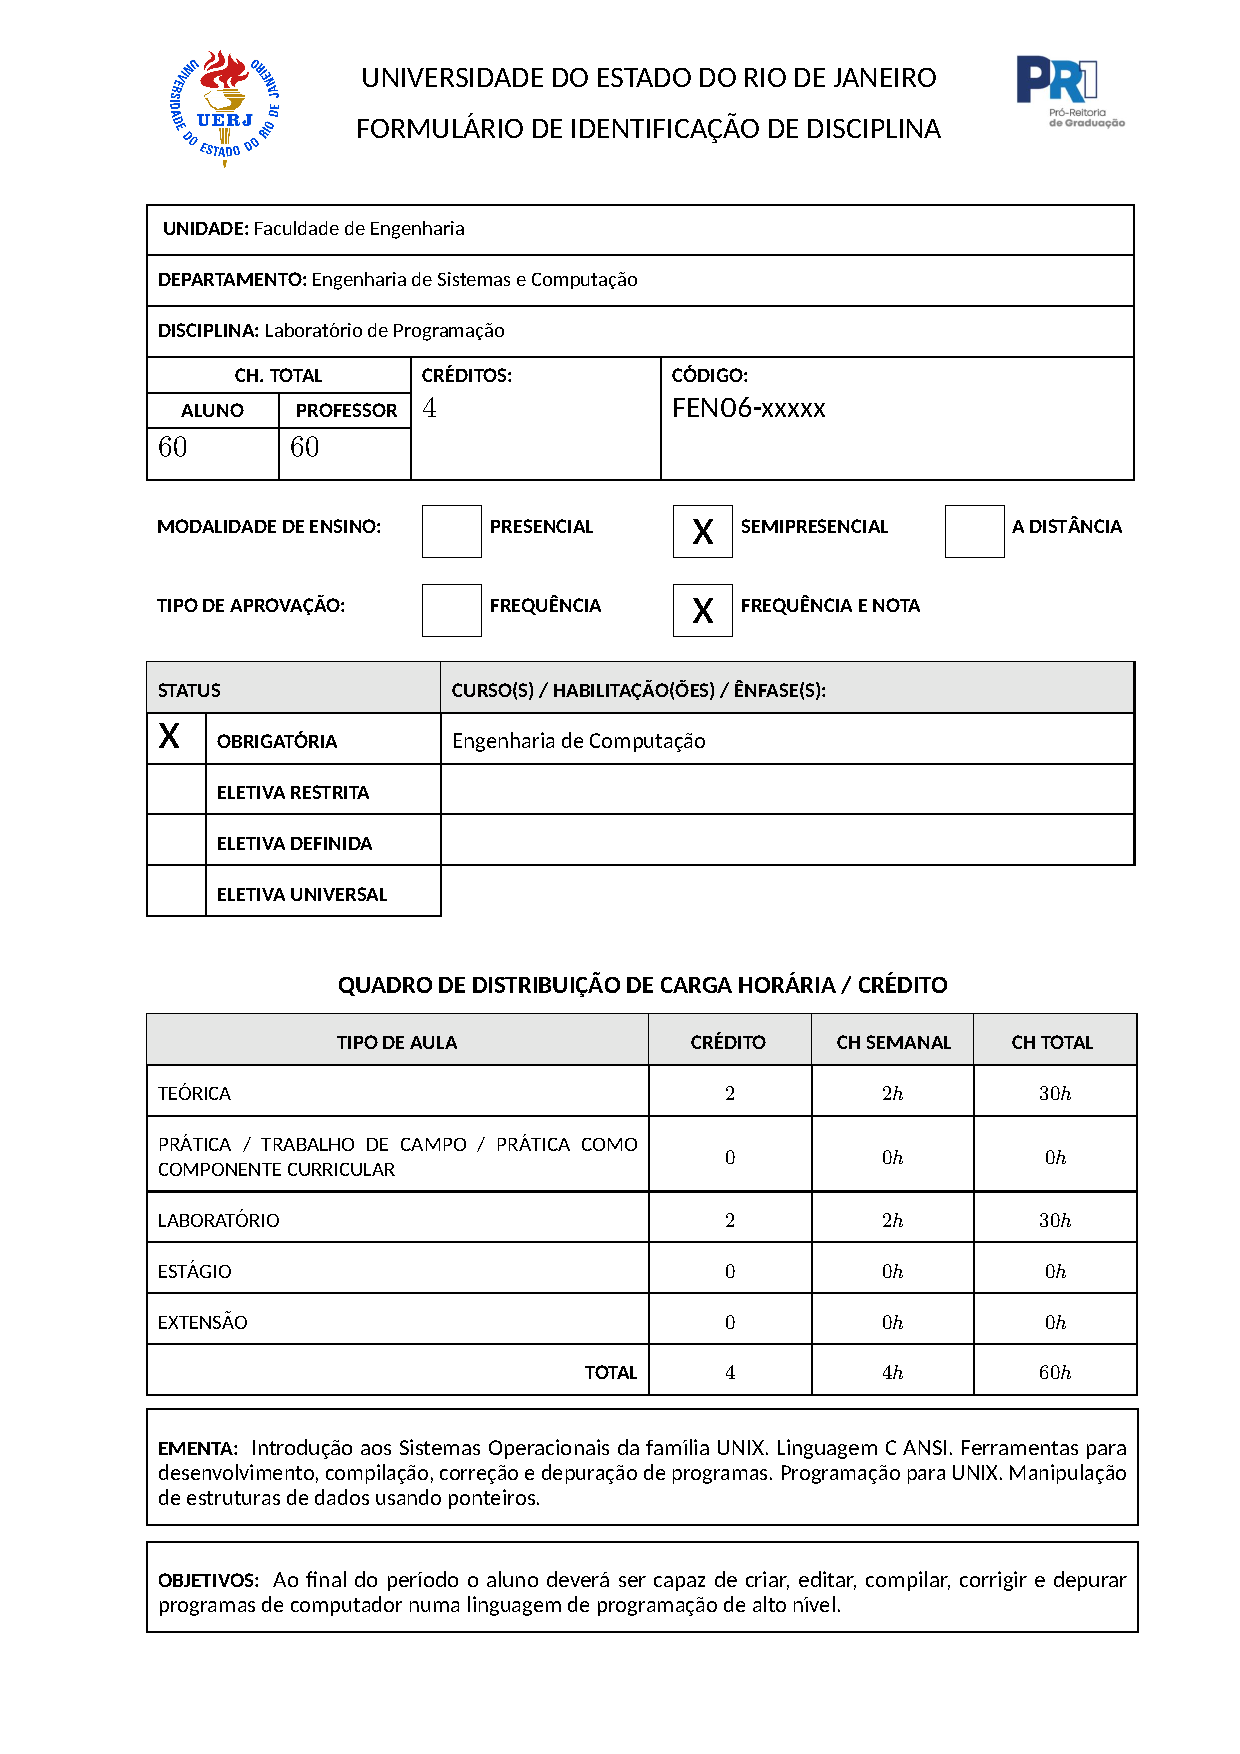
\includepdf[pages=-,addtotoc={1,section,1,{\LabProgA},},pagecommand={\thispagestyle{fancy}}]{ementas/LaboratorioDeProgramacaoA.pdf}
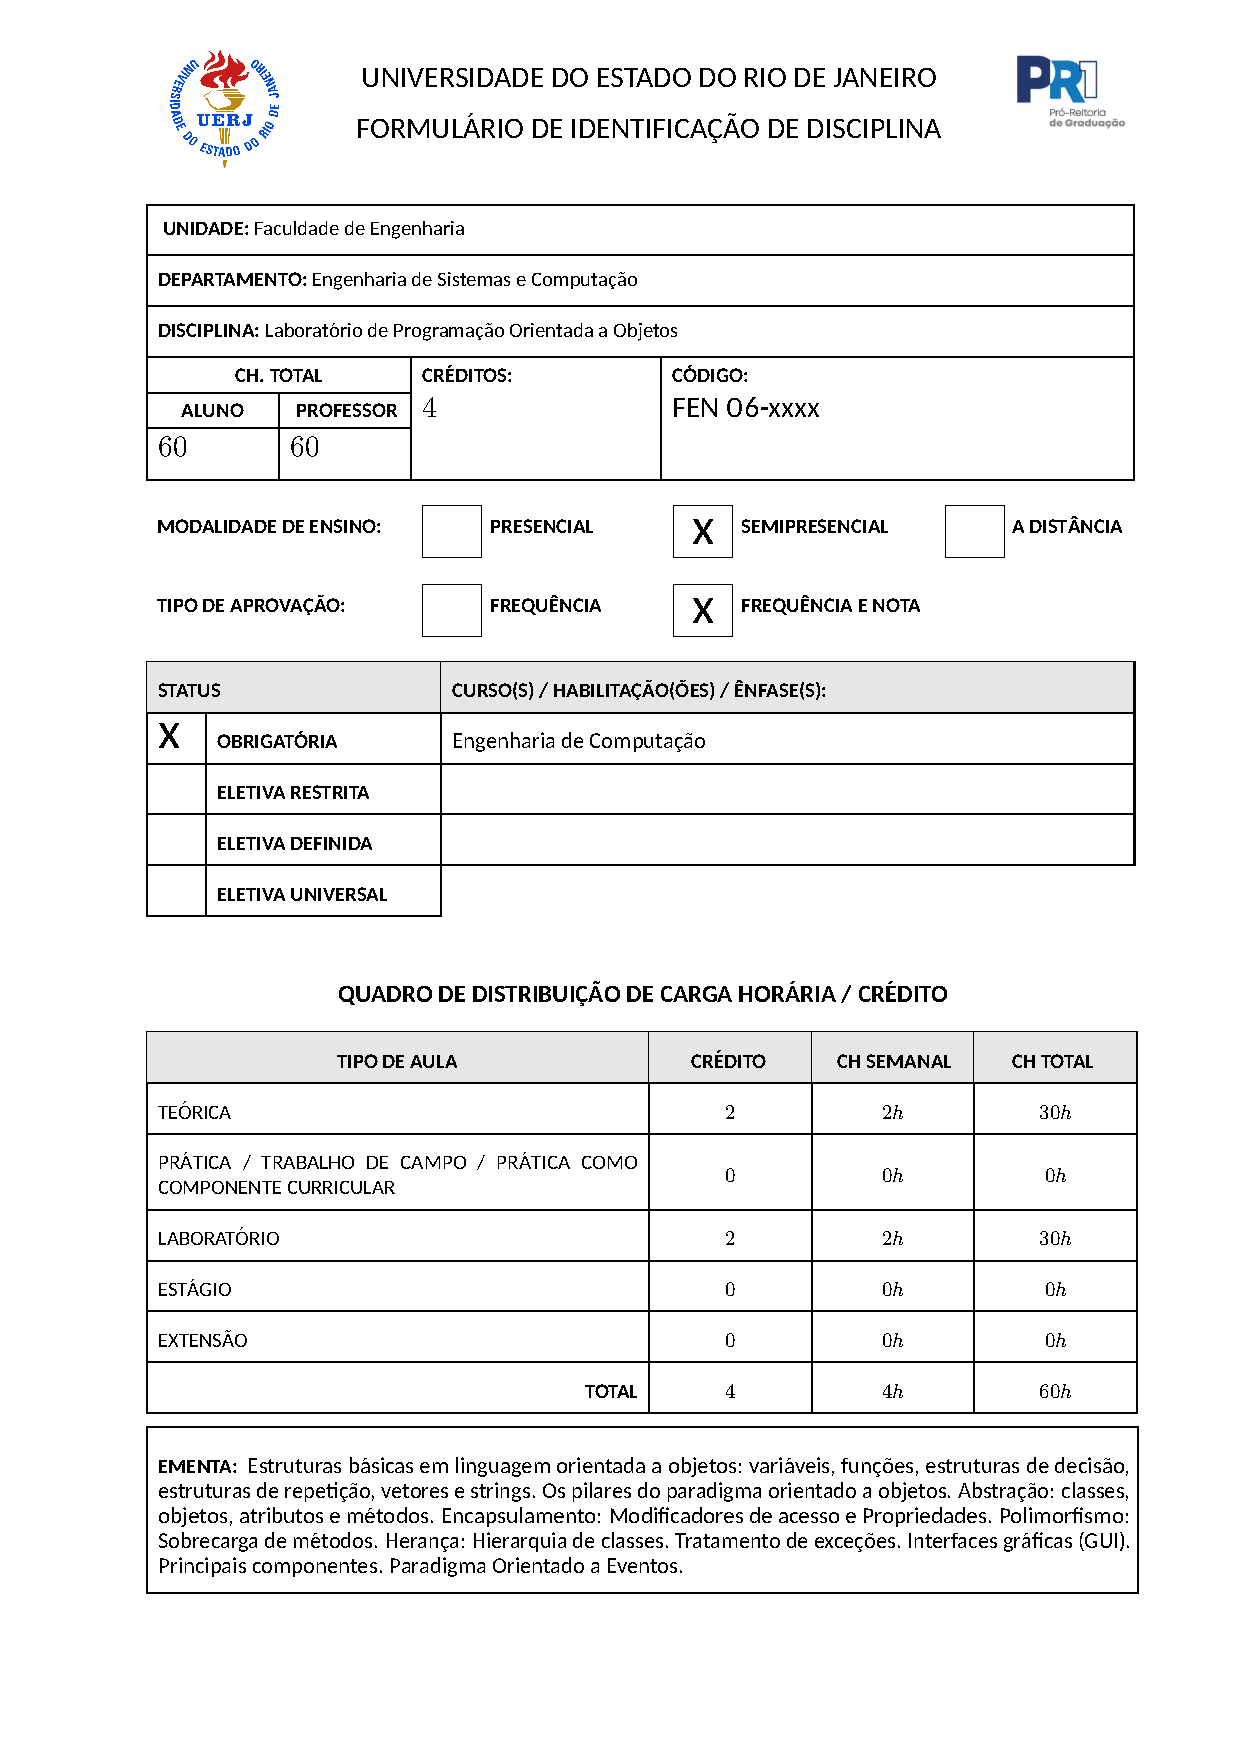
\includepdf[pages=-,addtotoc={1,section,1,{\LabProgPOO},},pagecommand={\thispagestyle{fancy}}]{ementas/LaboratorioDeProgramacaoB.pdf}
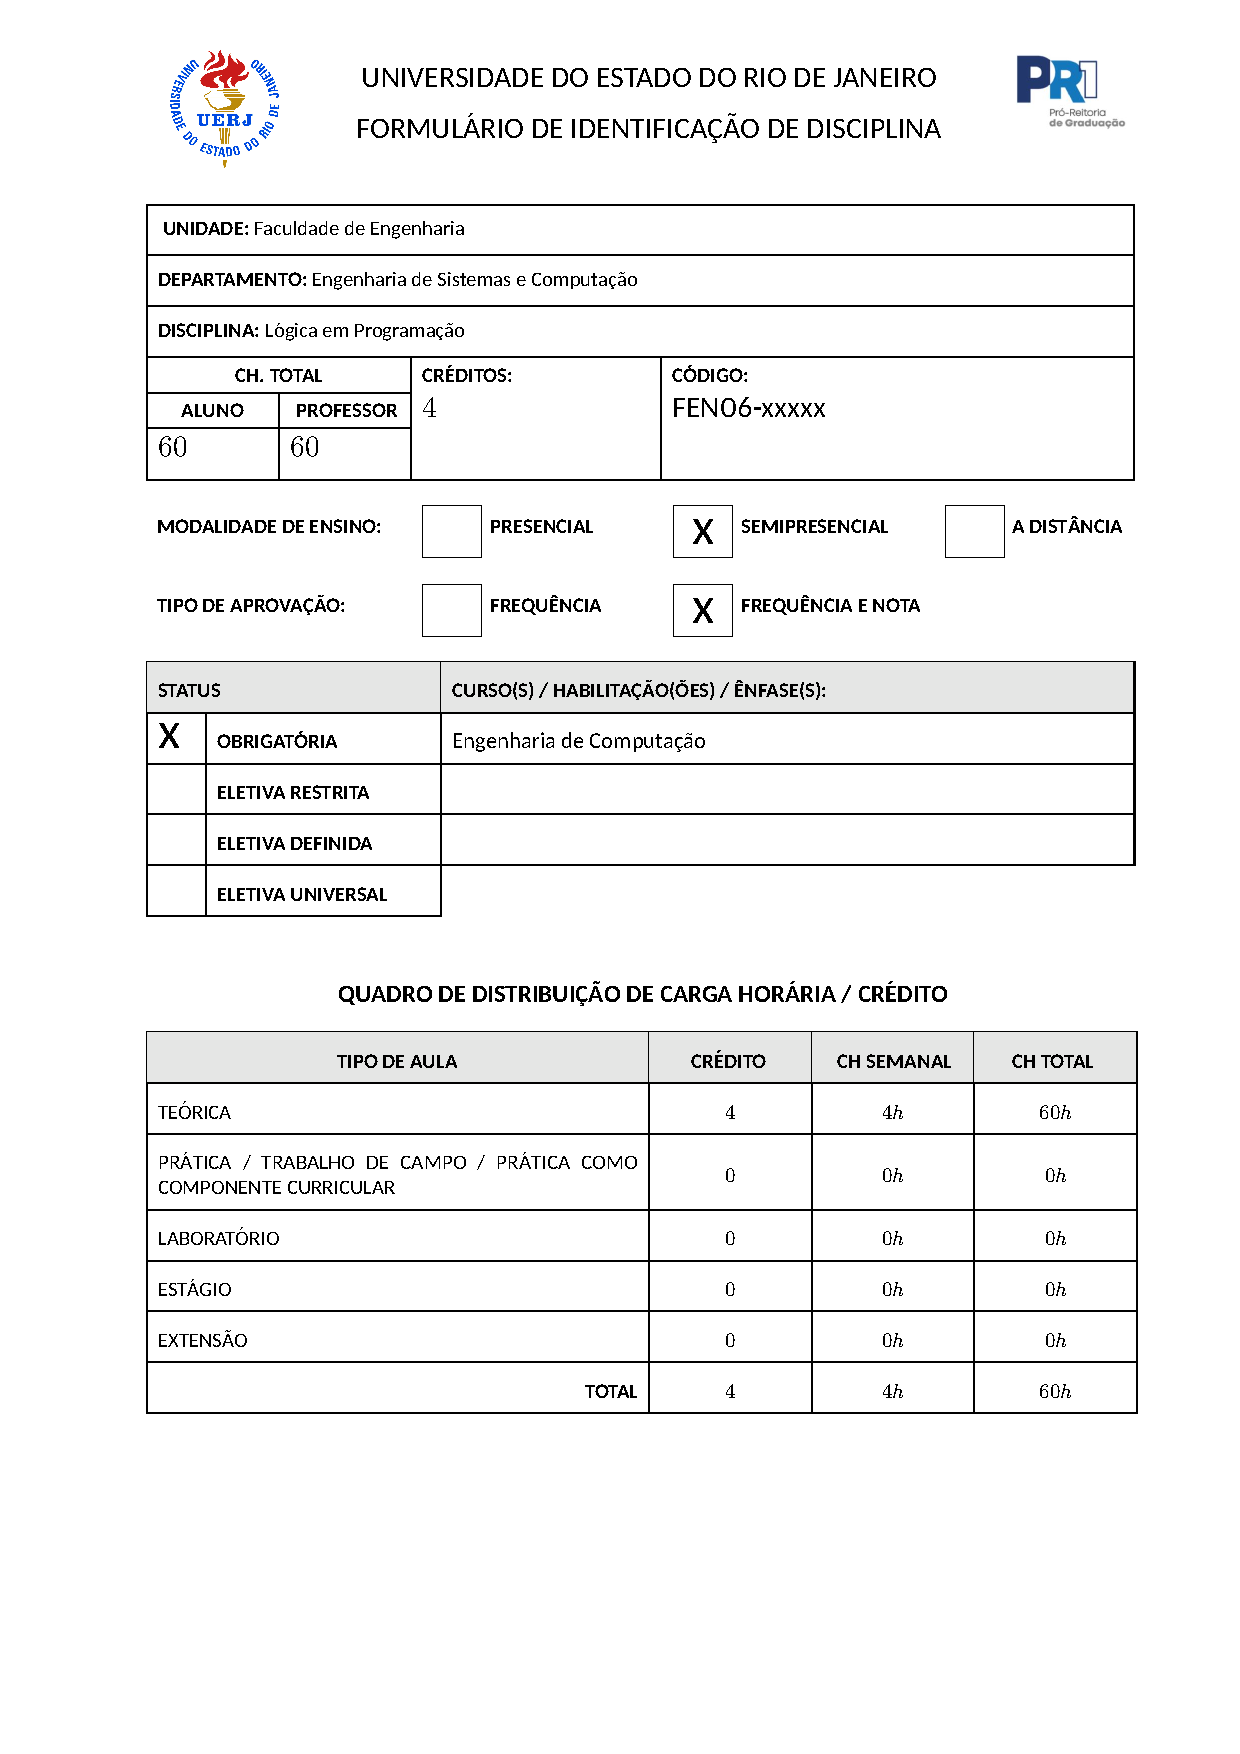
\includepdf[pages=-,addtotoc={1,section,1,{\LogProg},},pagecommand={\thispagestyle{fancy}}]{ementas/LogicaEmProgramacao.pdf}
\includepdf[pages=-,addtotoc={1,section,1,{\MacroEco},},pagecommand={\thispagestyle{fancy}}]{ementasExternas/macroeconomia_assinado.pdf} % Macroeconomia
\includepdf[pages=-,addtotoc={1,section,1,{\MatEle},},pagecommand={\thispagestyle{fancy}}]{ementasExternas/FEN05-Materiais_eletricos_e_Eletronicos_assinado.pdf}
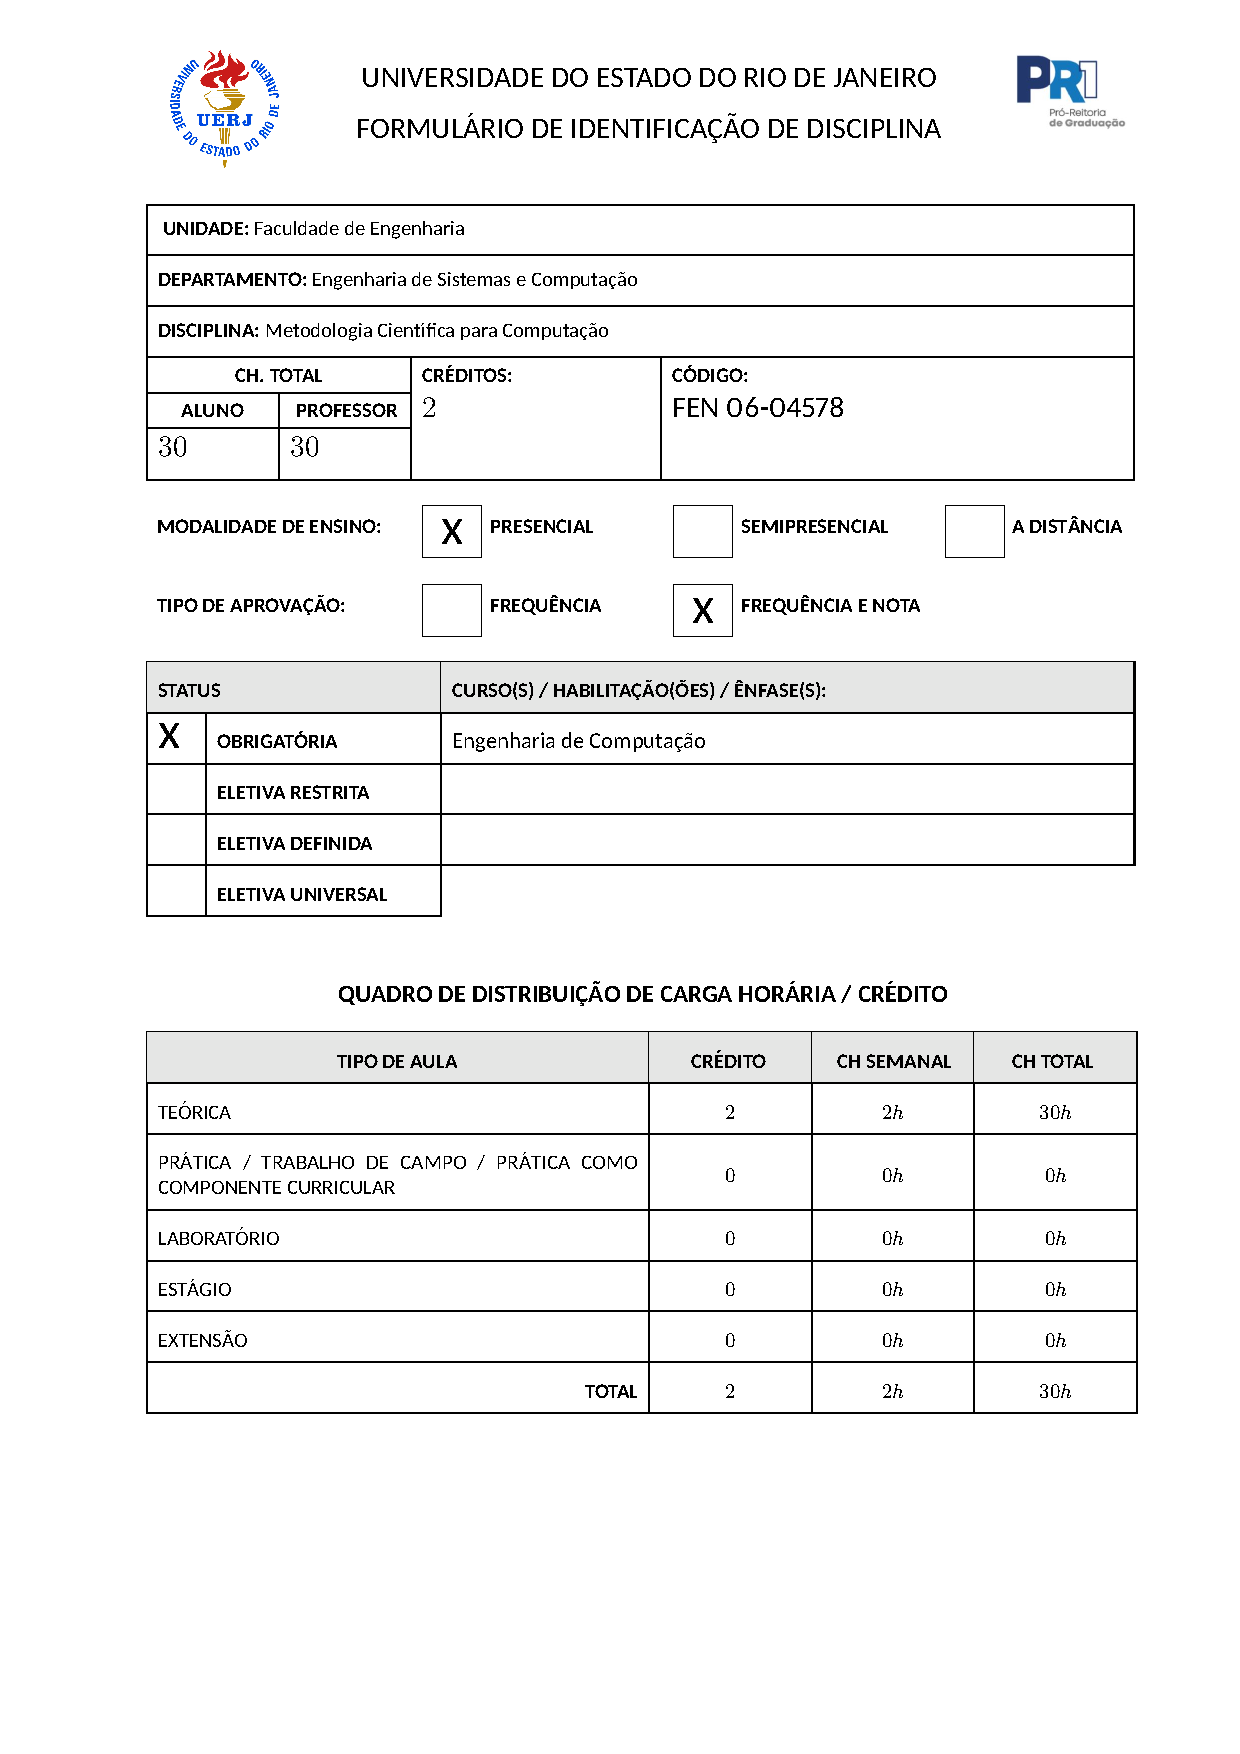
\includepdf[pages=-,addtotoc={1,section,1,{\ProjA},},pagecommand={\thispagestyle{fancy}}]{ementas/ProjetoXIA.pdf} %  Metodo de Projeto 
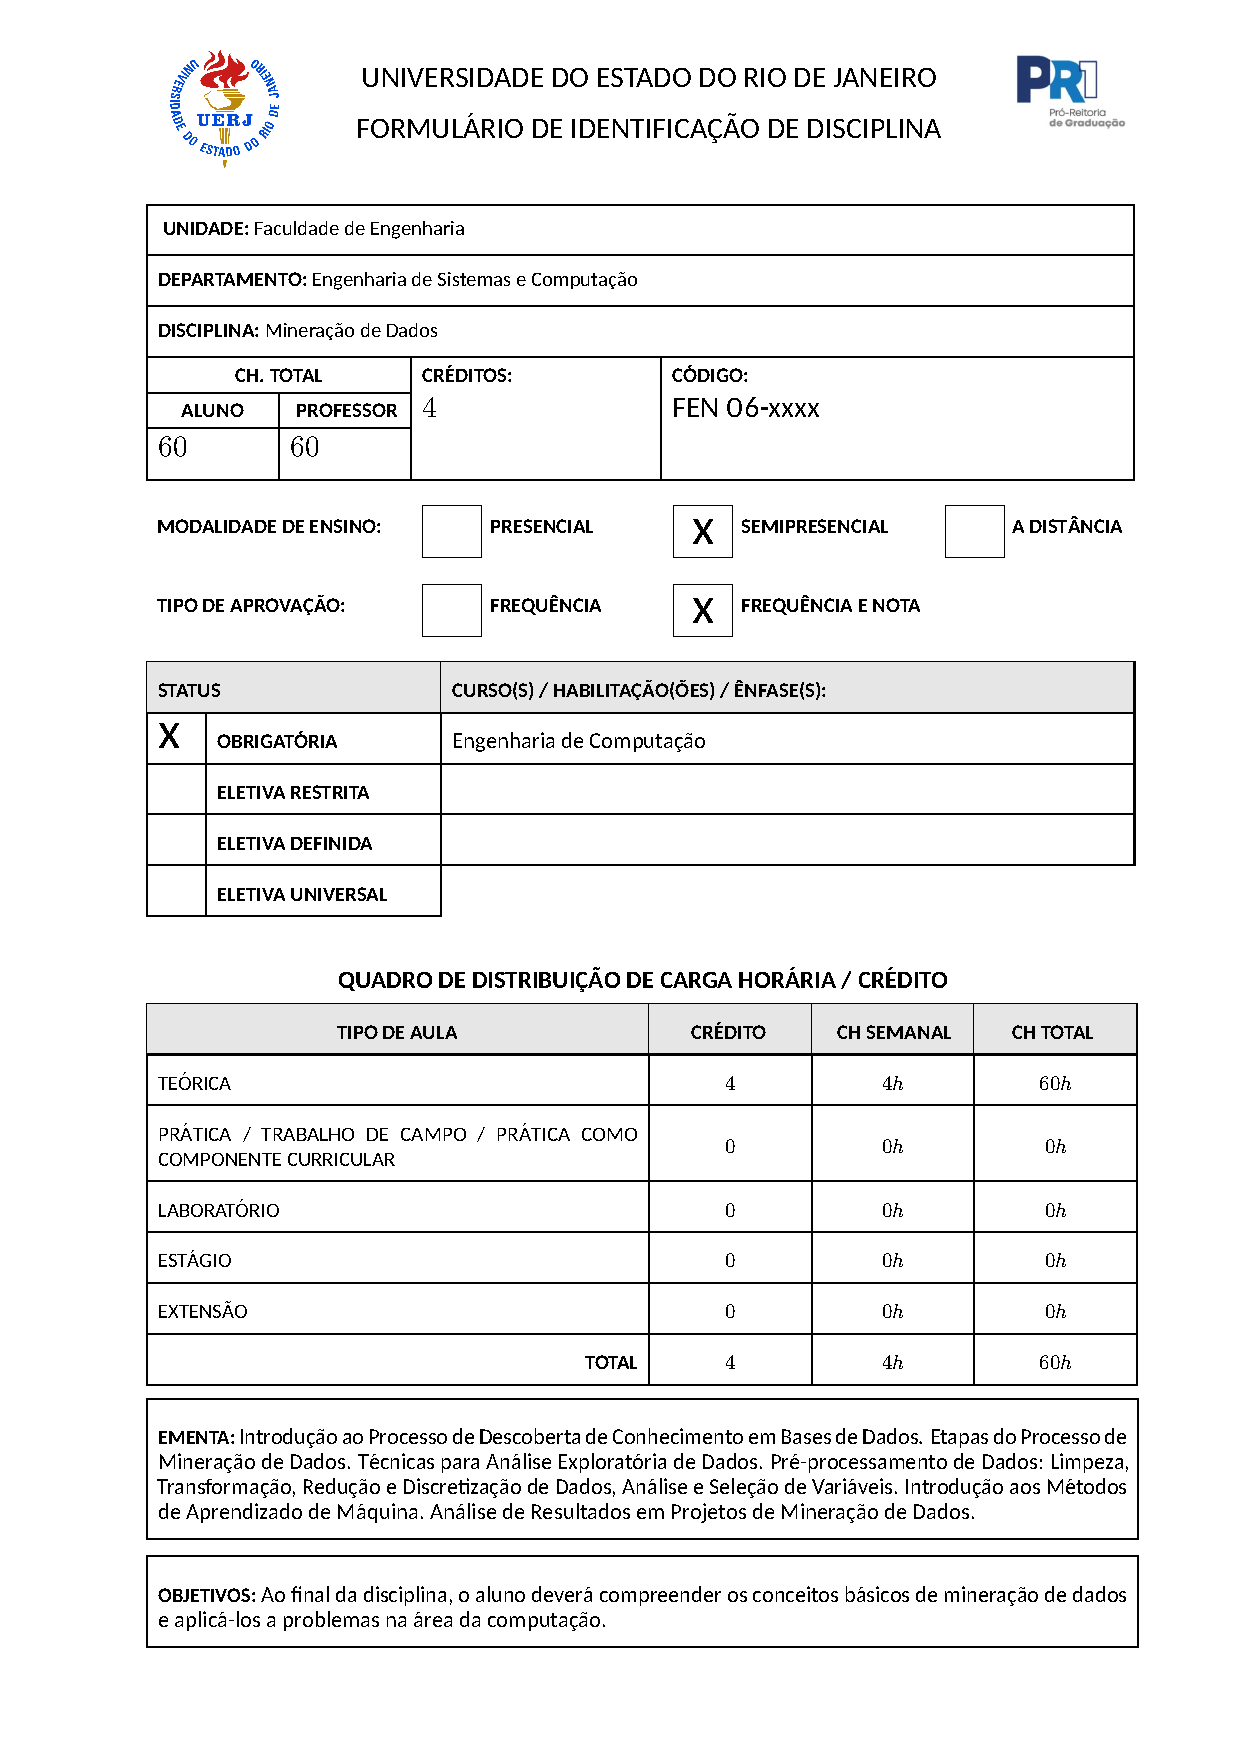
\includepdf[pages=-,addtotoc={1,section,1,{\MineraDados},},pagecommand={\thispagestyle{fancy}}]{ementas/MineracaoDeDados.pdf}
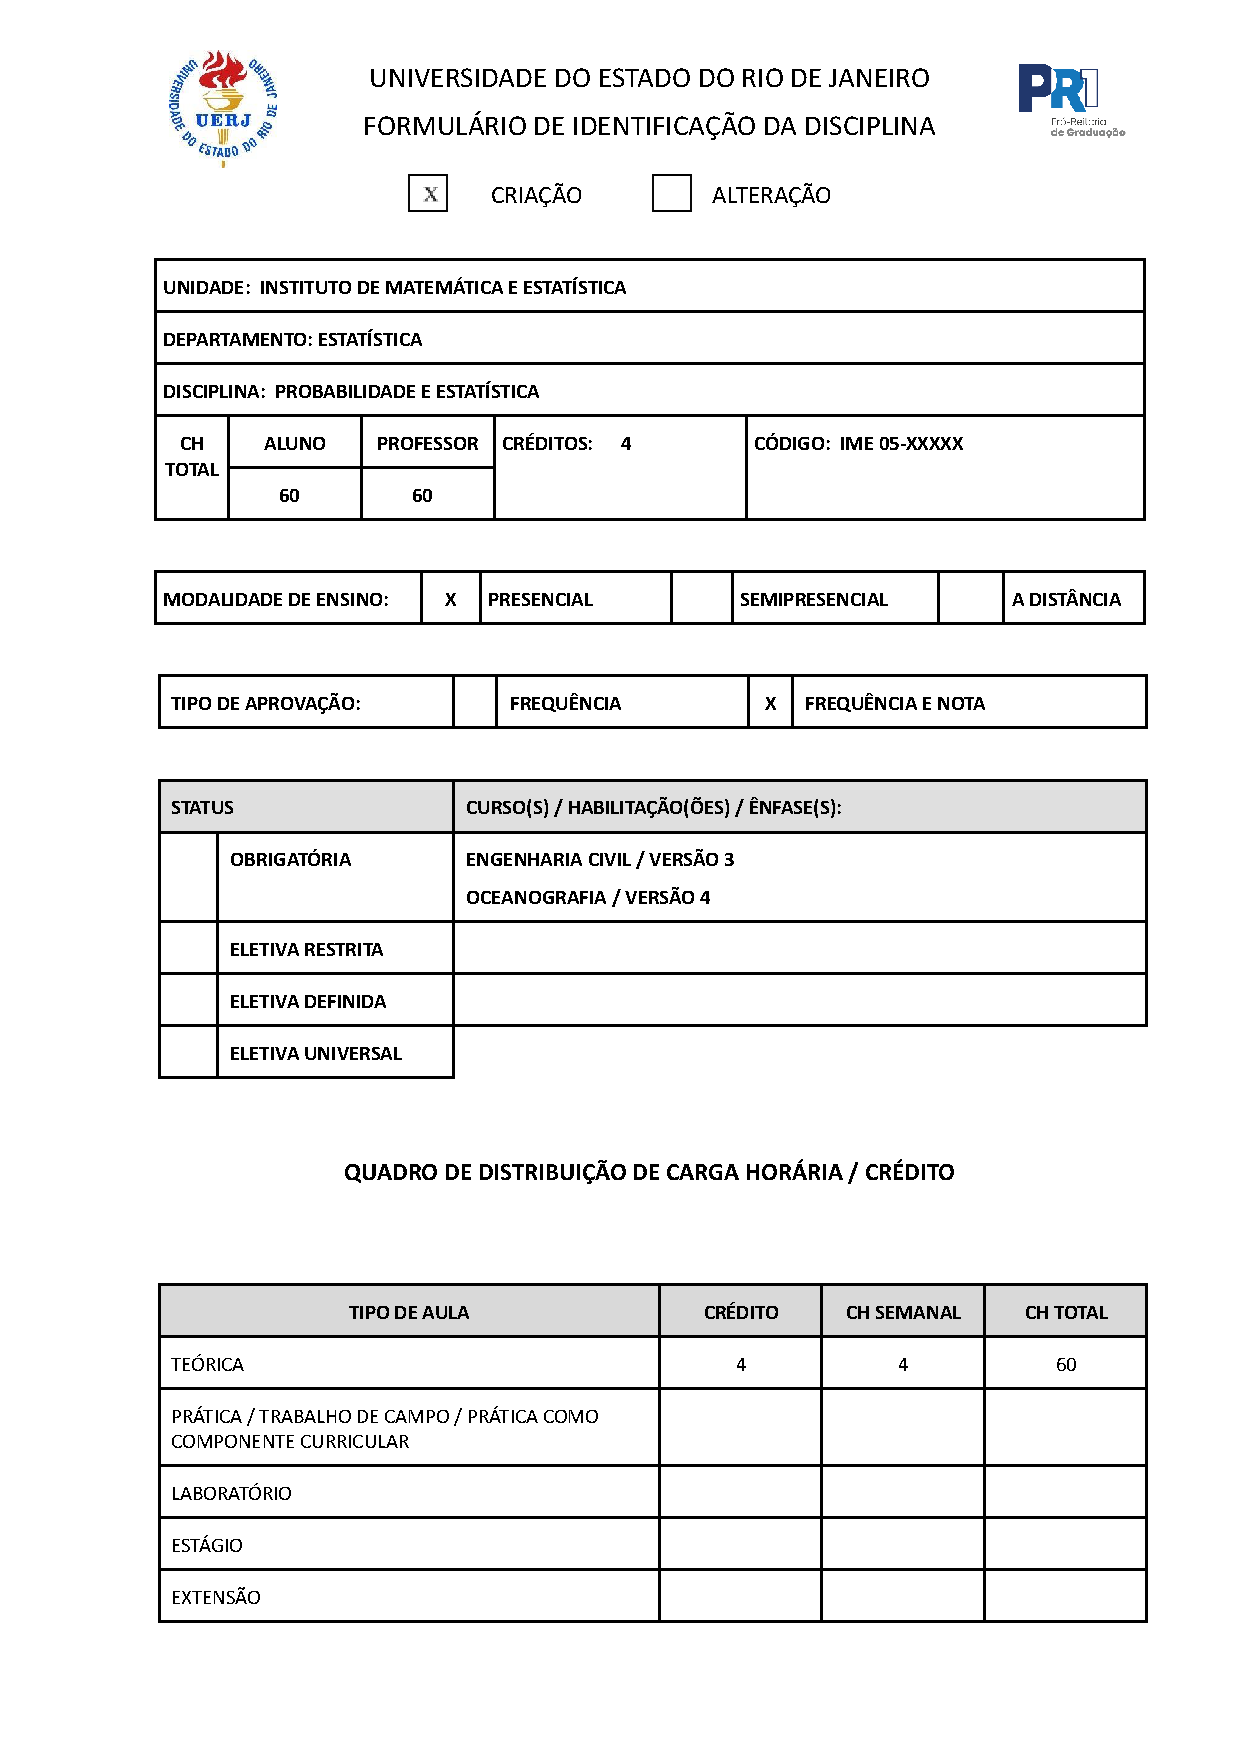
\includepdf[pages=-,addtotoc={1,section,1,{\ProbEst},},pagecommand={\thispagestyle{fancy}}]{ementasExternas/Probabilidade_e_Estatistica.pdf}
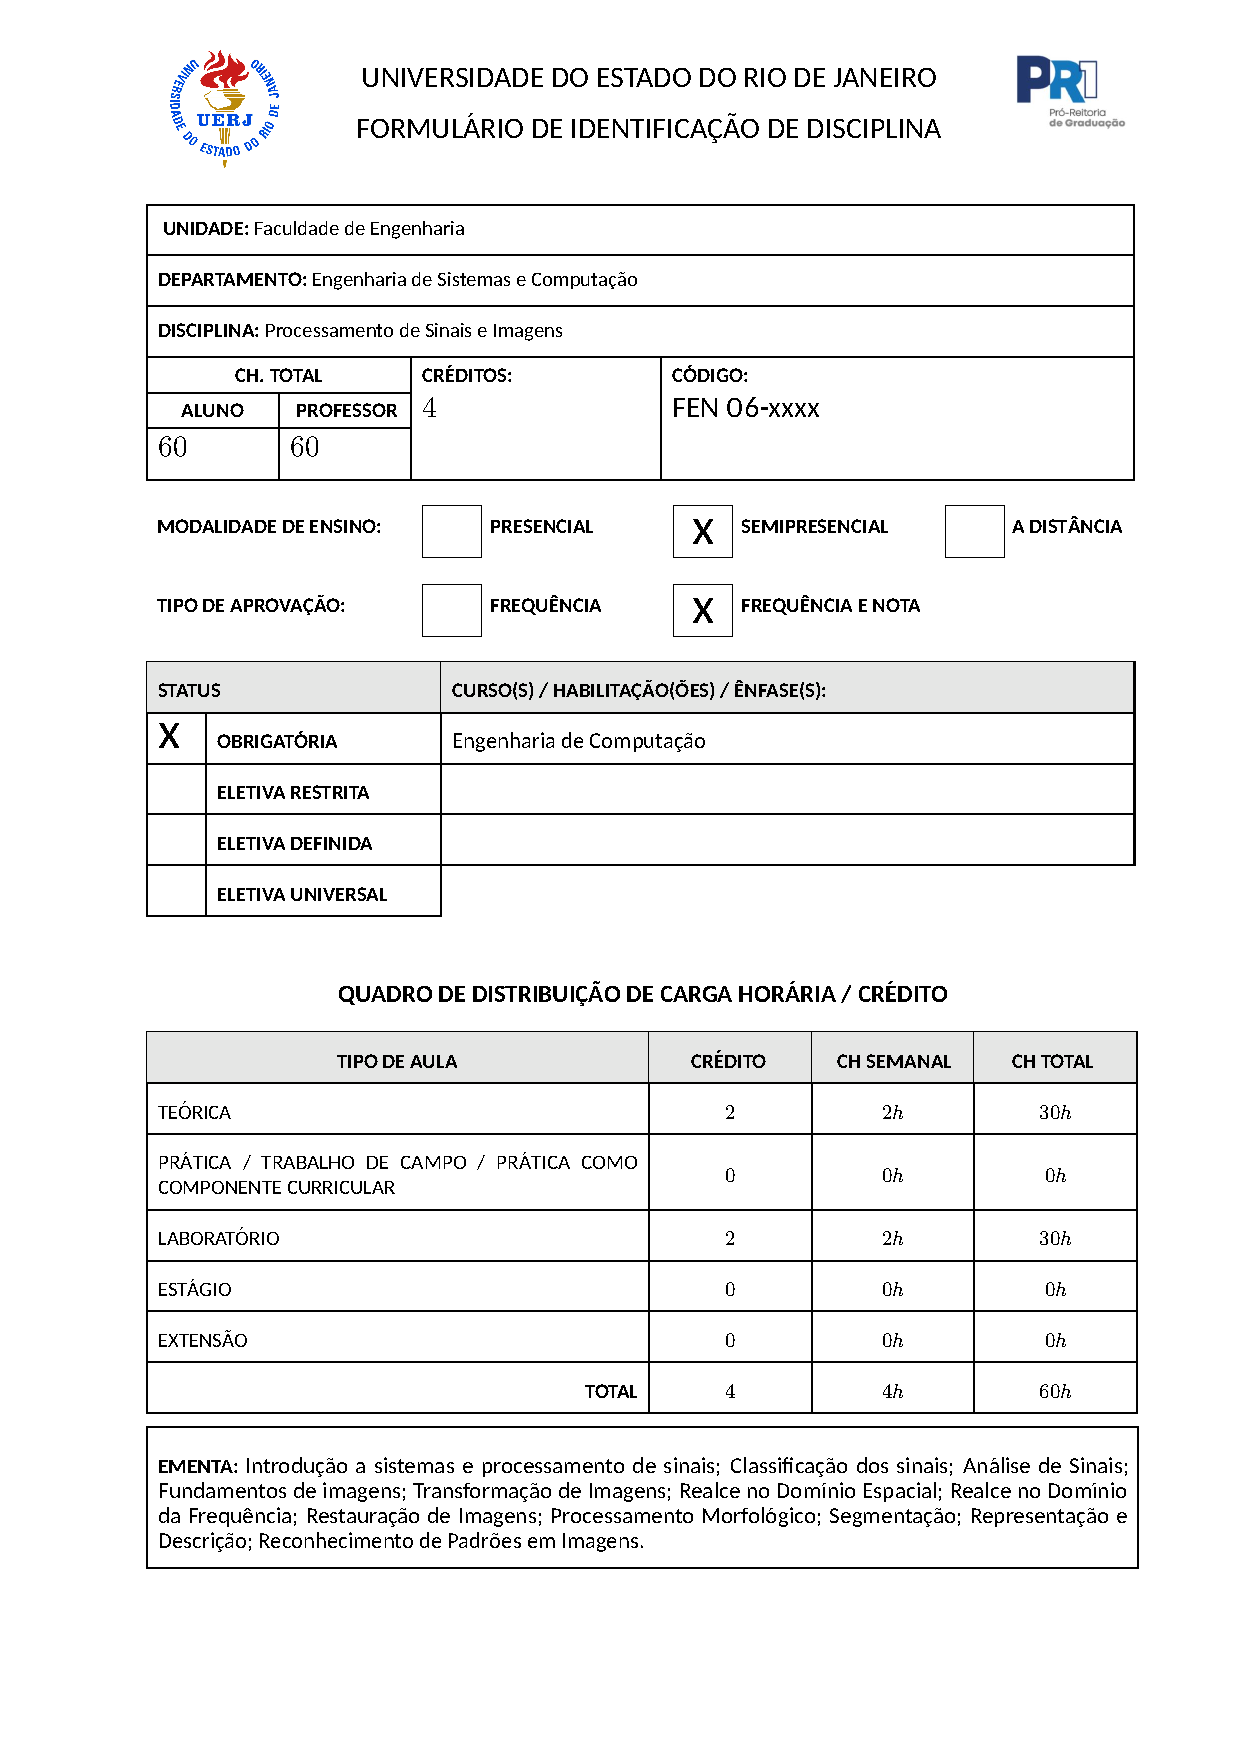
\includepdf[pages=-,addtotoc={1,section,1,{\ProcImag},},pagecommand={\thispagestyle{fancy}}]{ementas/ProcessamentoDeImagens.pdf}
\includepdf[pages=-,addtotoc={1,section,1,{\ProjBD},},pagecommand={\thispagestyle{fancy}}]{ementas/projeto_de_BD.pdf}
% Projetos de Extensão
\includepdf[pages=-,addtotoc={1,section,1,{\Ext},},pagecommand={\thispagestyle{fancy}}]{ementas/ProjetoDeExtensao.pdf}
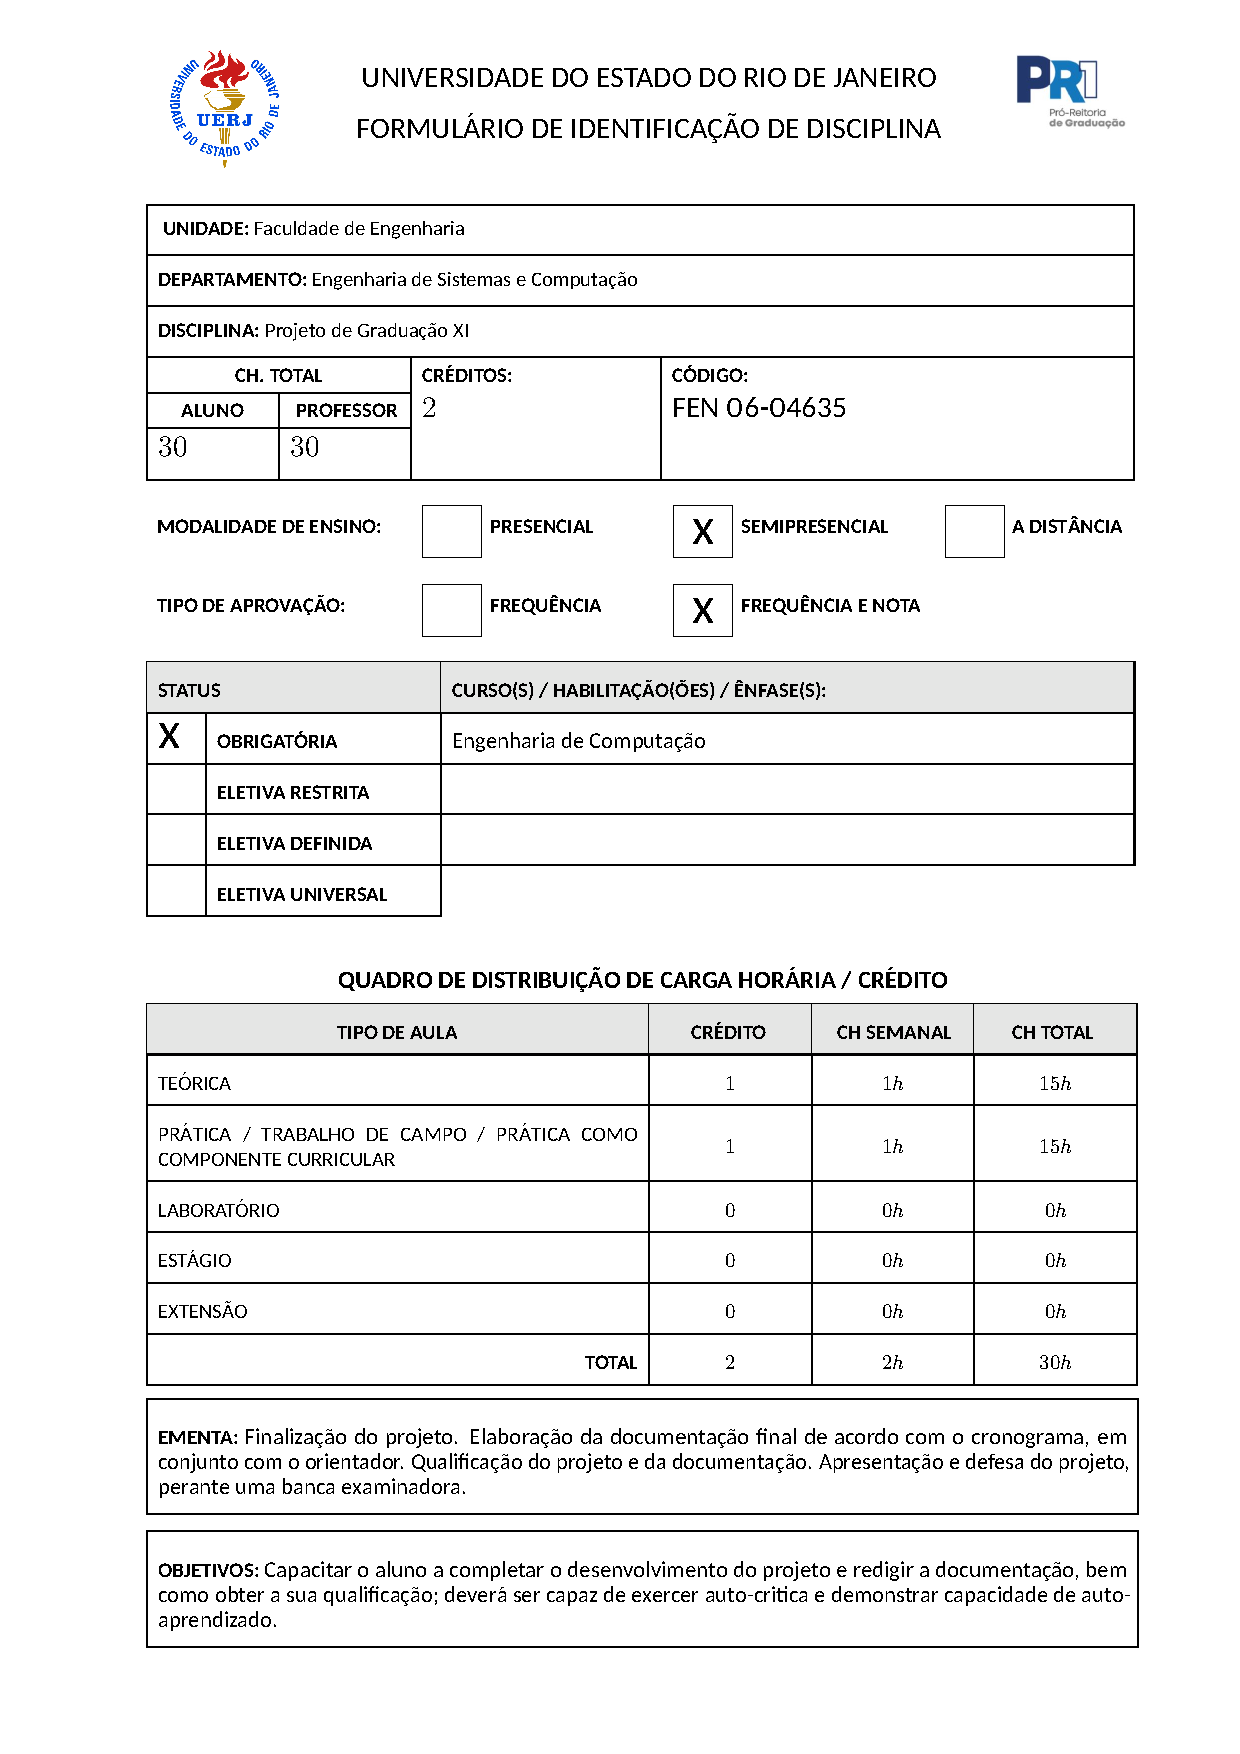
\includepdf[pages=-,addtotoc={1,section,1,{\ProjB},},pagecommand={\thispagestyle{fancy}}]{ementas/ProjetoXIB.pdf}
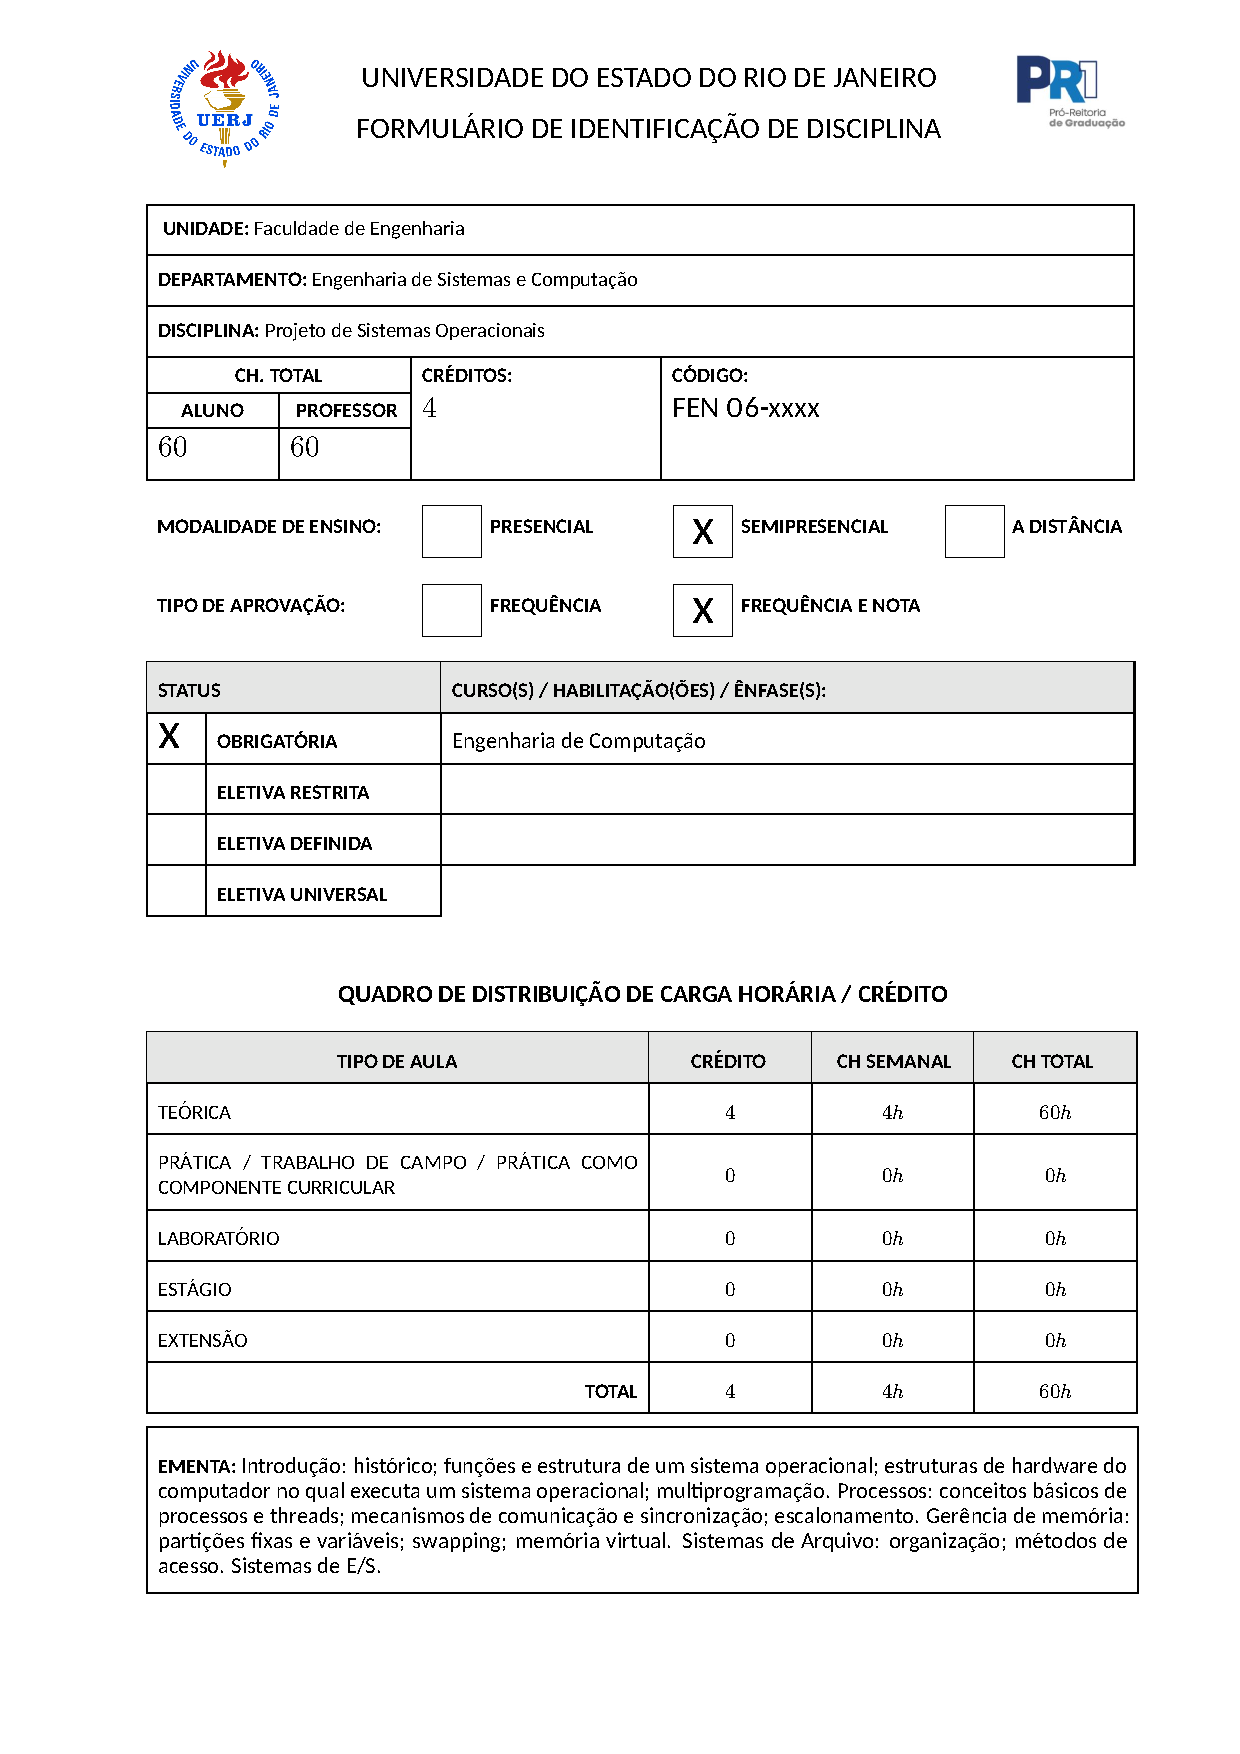
\includepdf[pages=-,addtotoc={1,section,1,{\ProjSO},},pagecommand={\thispagestyle{fancy}}]{ementas/ProjetoDeSistemasOperacionais.pdf}
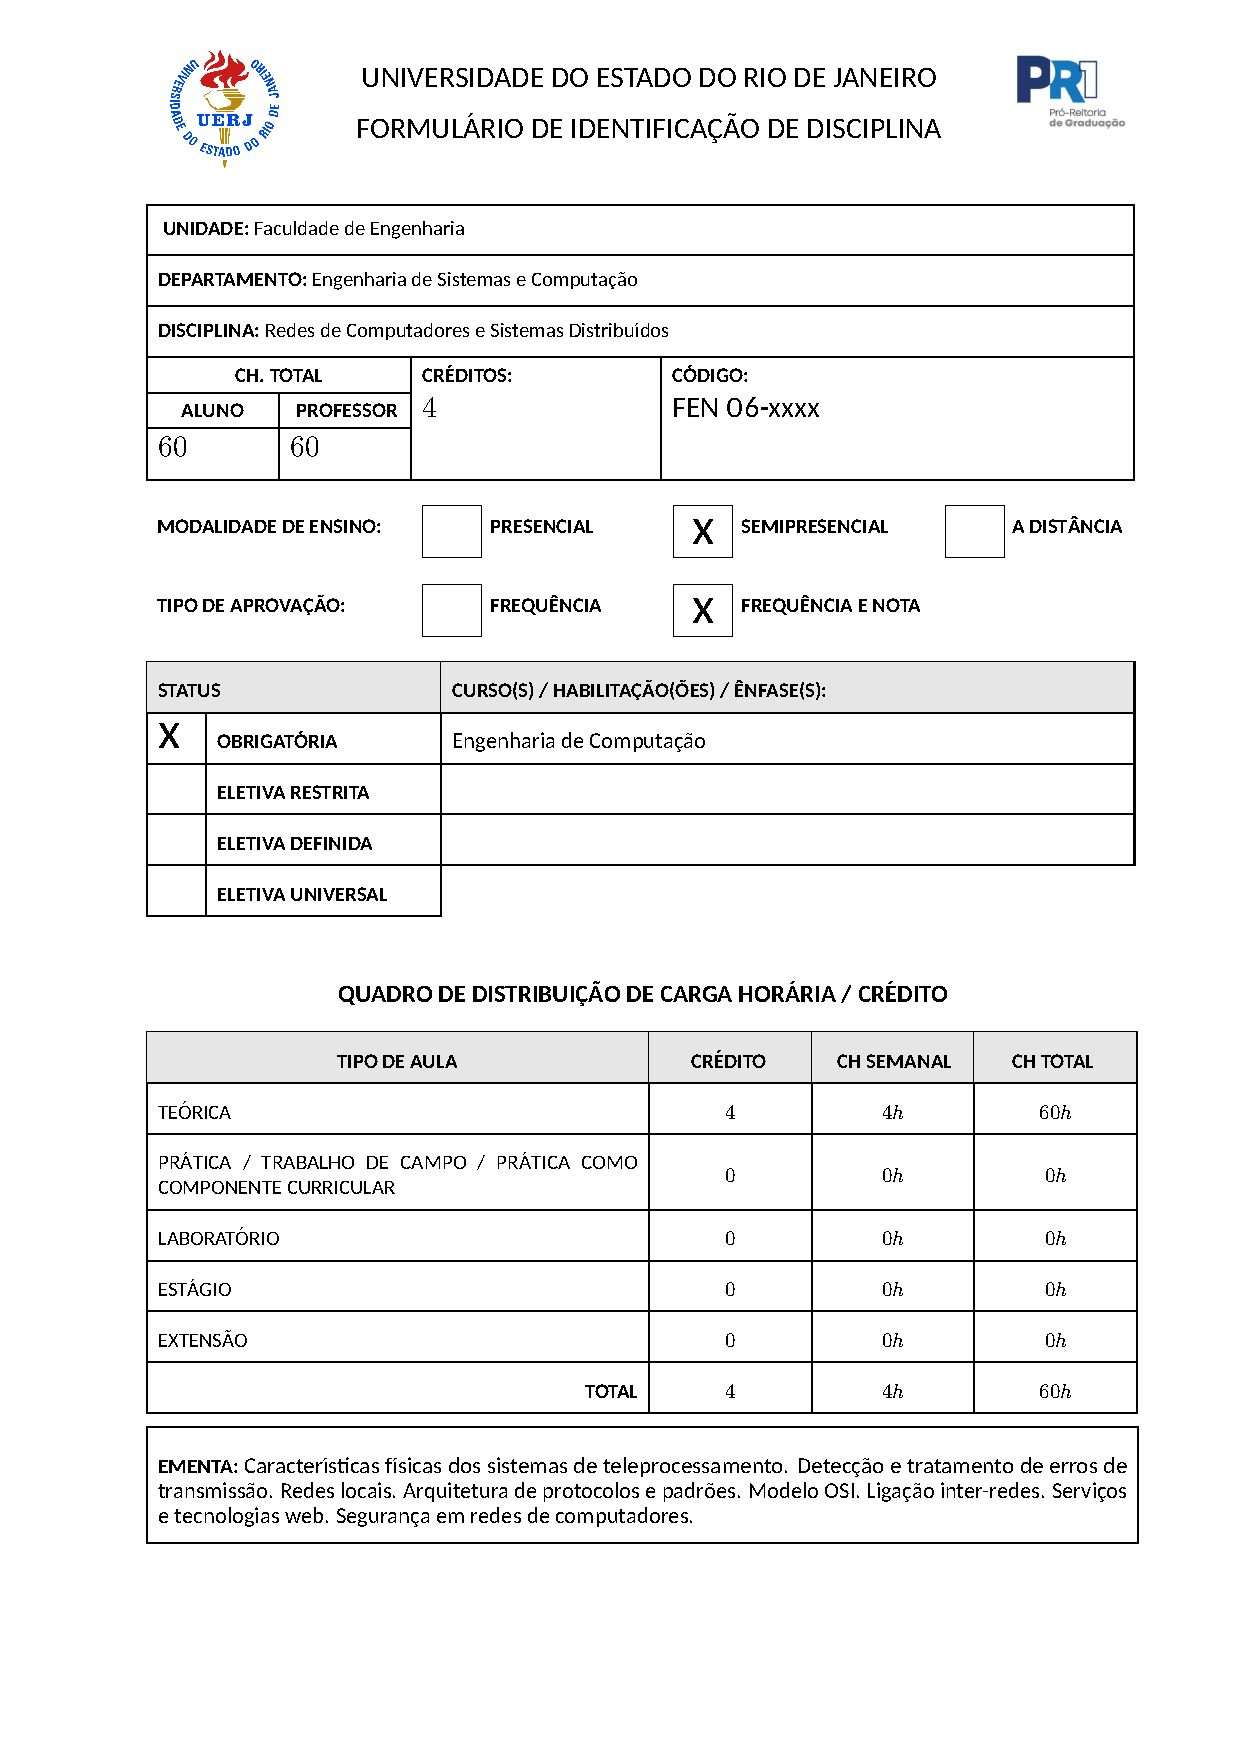
\includepdf[pages=-,addtotoc={1,section,1,{\Telep},},pagecommand={\thispagestyle{fancy}}]{ementas/TeleprocessamentoERedes.pdf} % Redes de Computadores e Sistemas Distribuídos
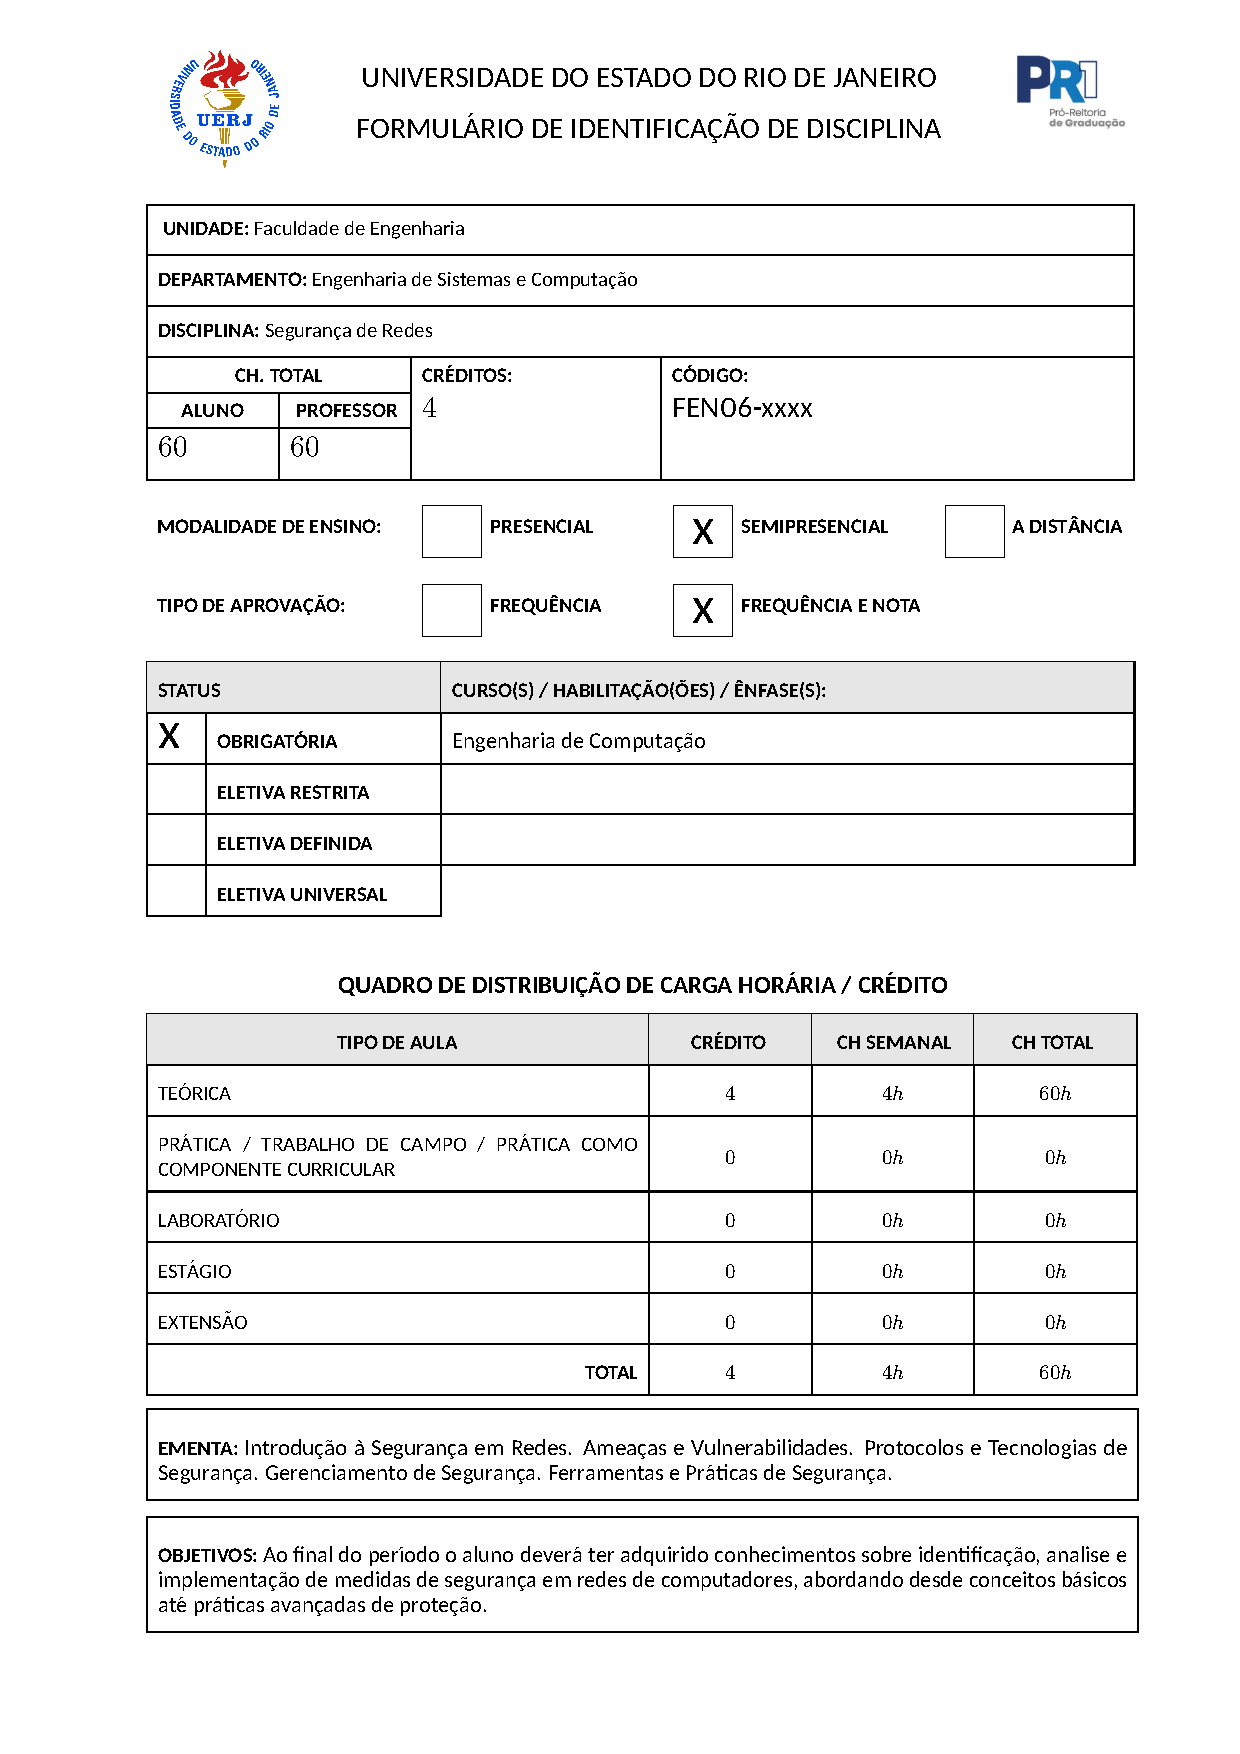
\includepdf[pages=-,addtotoc={1,section,1,{\Sredes},},pagecommand={\thispagestyle{fancy}}]{ementas/seguranca_de_redes.pdf}
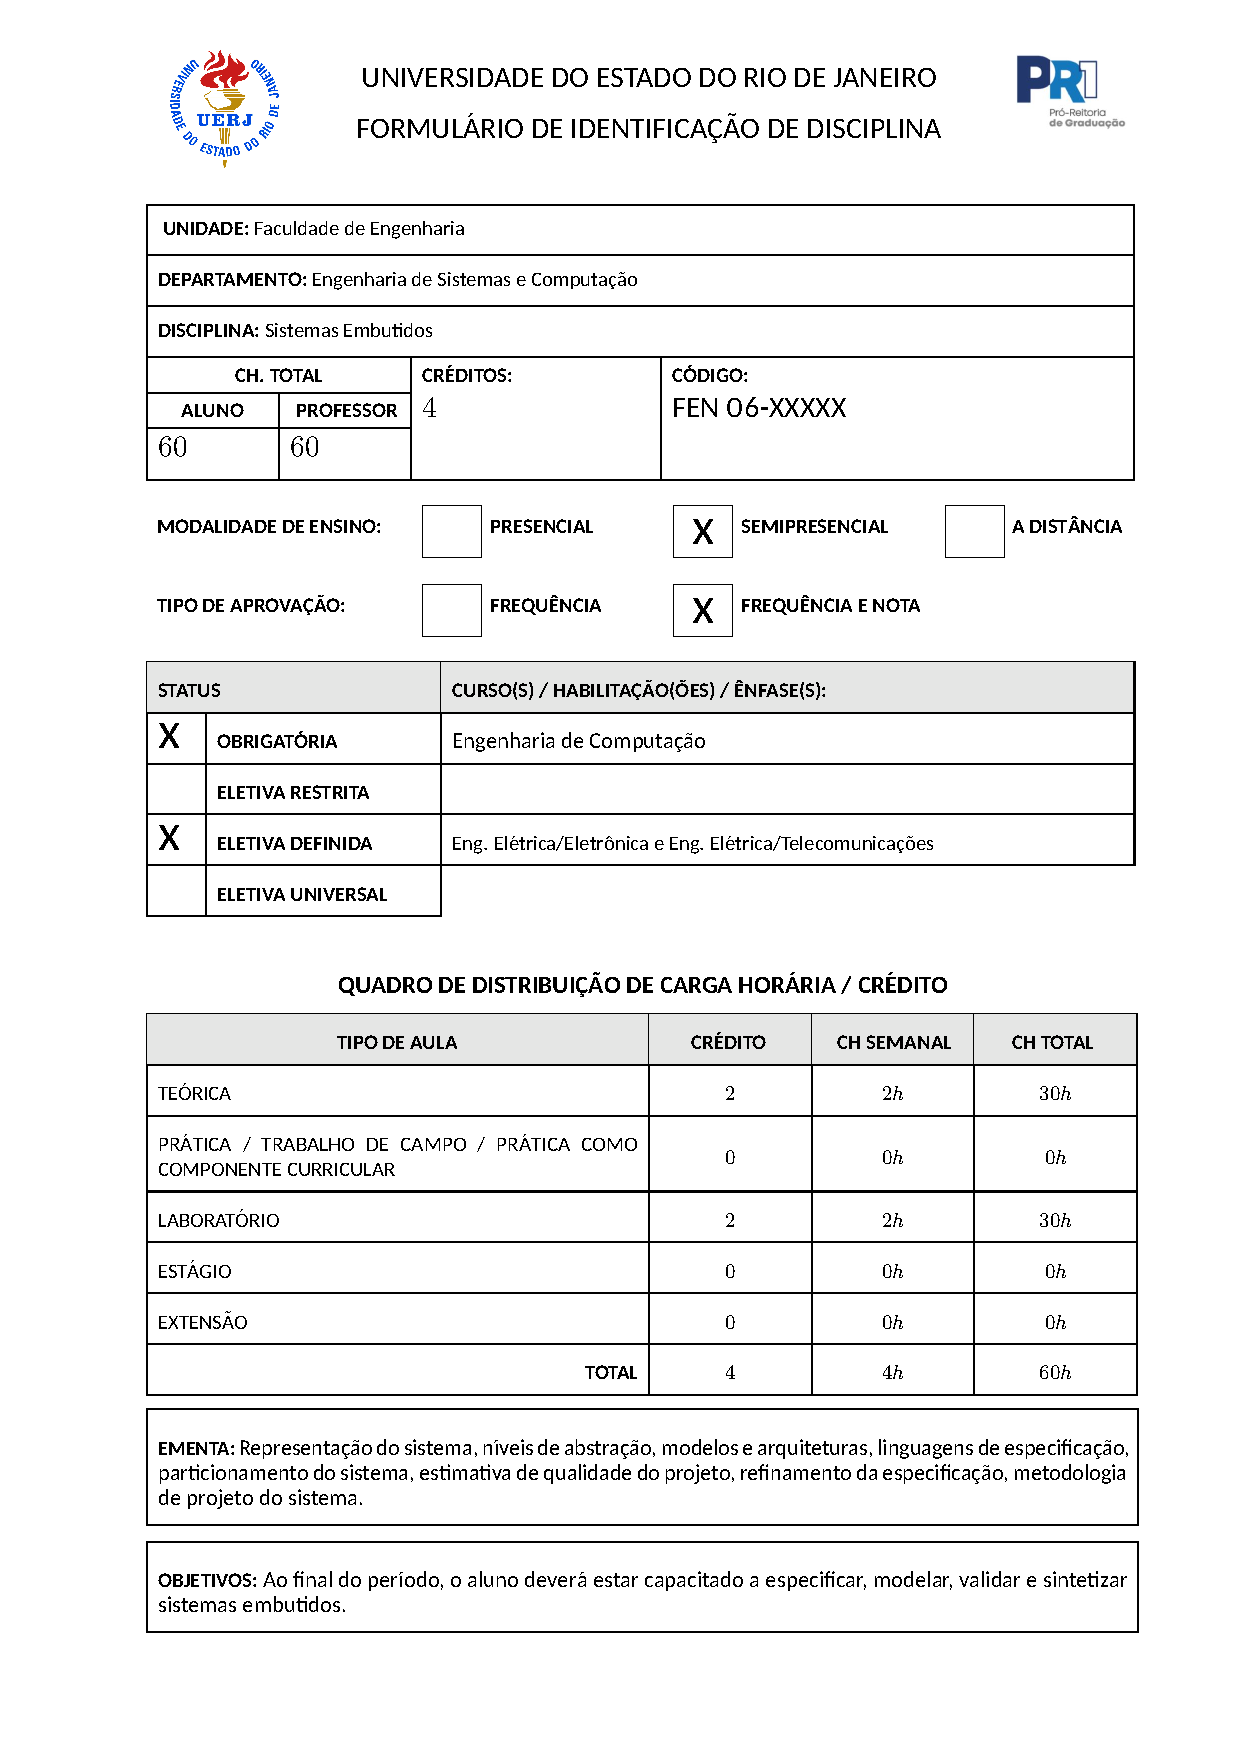
\includepdf[pages=-,addtotoc={1,section,1,{\SistEmb},},pagecommand={\thispagestyle{fancy}}]{ementas/SistemasEmbutidos.pdf}
% Técnicas Digitais
\includepdf[pages=-,addtotoc={1,section,1,{\TecDig},},pagecommand={\thispagestyle{fancy}}]{ementasExternas/FEN05-Tecnicas_Digitais_assinado.pdf}
\includepdf[pages=-,addtotoc={1,section,1,{\TeoComp},},pagecommand={\thispagestyle{fancy}}]{ementas/TeoriaDeCompiladores.pdf}
\includepdf[pages=-,addtotoc={1,section,1,{\Grafos},},pagecommand={\thispagestyle{fancy}}]{ementas/TeoriadosGrafos.pdf}


\chapter{Ementas de Disciplinas Eletivas}
% \includepdf[pages=-,addtotoc={1,section,1,{\EletRec},},pagecommand={\thispagestyle{fancy}}]{Eletiva1_ReconhecimentoDePadroes.pdf}
% Aprendizado por Reforço
\includepdf[pages=-,addtotoc={1,section,1,{\EletReforco},},pagecommand={\thispagestyle{fancy}}]{ementas/e_aprendizado_por_reforco.pdf}
% Processamento de Linguagem Natural
\includepdf[pages=-,addtotoc={1,section,1,{\AprendProfPLN},},pagecommand={\thispagestyle{fancy}}]{ementas/e_aprendizadoPLN.pdf}
% Aprendizado Profundo para Visão Computacional
\includepdf[pages=-,addtotoc={1,section,1,{\EletVisao},},pagecommand={\thispagestyle{fancy}}]{ementas/e_visao_computacional.pdf}
% Automação de Processos Robóticos
\includepdf[pages=-,addtotoc={1,section,1,{\AutomProcRob},},pagecommand={\thispagestyle{fancy}}]{ementas/e_automacao_processos_roboticos.pdf}
% Arquiteturas Avançadas de Computadores
\includepdf[pages=-,addtotoc={1,section,1,{\EletArq},},pagecommand={\thispagestyle{fancy}}]{ementas/e_arquiteturas_avancadas.pdf}
% Geomática
\includepdf[pages=-,addtotoc={1,section,1,{\EletGeo},},pagecommand={\thispagestyle{fancy}}]{ementas/e_geoinformatica.pdf}
% Redes de Interconexão
\includepdf[pages=-,addtotoc={1,section,1,{\EletRedes},},pagecommand={\thispagestyle{fancy}}]{ementas/e_redes_interconexao.pdf}
% Sistemas Operacionais para Robótica Inteligente
\includepdf[pages=-,addtotoc={1,section,1,{\SistOpRobInt},},pagecommand={\thispagestyle{fancy}}]{ementas/e_so_robotica.pdf}
% Técnicas de Programação em Otimização Combinatória
\includepdf[pages=-,addtotoc={1,section,1,{\TecProgOtim},},pagecommand={\thispagestyle{fancy}}]{ementas/e_tecnicas_POC.pdf}
% Tópicos Especiais em Visão Computacional

% Legislação
\includepdf[pages=-,addtotoc={1,section,1,{\TopEspVisComp},},pagecommand={\thispagestyle{fancy}}]{ementas/e_te_em_visao_computacional.pdf}
% Institui as Diretrizes Curriculares Nacionais para os cursos de graduação na área da Computação
\chapter{Resolução CNE/CES n\textordmasculine{} 5, de 16 de novembro de 2016}
\label{cne2016}
\includepdf[pages=-,pagecommand={\thispagestyle{fancy}}]{leis/rces005_16.pdf}
% Referenciais SBC para cursos de Computação
\chapter{SBC: Referenciais para Graduação em Computação}
\label{sbc2017}
\includepdf[pages=-,pagecommand={\thispagestyle{fancy}}]{leis/sbc2017.pdf}
% Resolução CNE/CES n. 7/2018, que estabelece as as Diretrizes para a Extensão na Educação Superior Brasileira
\chapter{RESOLUÇÃO N\textordmasculine{} 7, DE 18 DE DEZEMBRO DE 2018 - CNE/CES}
\label{rcne2018}
\includepdf[pages=-,pagecommand={\thispagestyle{fancy}}]{leis/rces007_18.pdf}
% Deliberação n. 33/95, regras gerais de graduação UERJ
\chapter{Deliberação n\textordmasculine{} 33/95 da UERJ}
\label{delib3395}
\includepdf[pages=-,pagecommand={\thispagestyle{fancy}}]{leis/del-uerj1995.pdf}
% Deliberação n. 59/2019 da UERJ que altera a Deliberação n. 33/95 
\chapter{Deliberação n\textordmasculine{} 59/2019 da UERJ}
\label{delib592019}
\includepdf[pages=-,pagecommand={\thispagestyle{fancy}}]{leis/del-uerj2019.pdf}
% Deliberaçao n. 04/2023 do CSEPE/UERJ dispõe sobre inserção curricular da extensão na UERJ
\chapter{Deliberação n\textordmasculine{} 04/2023 do CSEPE/UERJ}
\label{del4}
\includepdf[pages=-,pagecommand={\thispagestyle{fancy}}]{leis/del-uerj2023.pdf}
%  Resolução n. 380/1993 CREA/CONFEA. Discrimina as atribuições do Engenheiro de Computação
\chapter{Resolução n\textordmasculine{} 380/1993 CREA/CONFEA}
\label{confea1993}
\includepdf[pages=1,pagecommand={\thispagestyle{fancy}}]{leis/confea93.pdf}
